\documentclass[]{article}
\usepackage{lmodern}
\usepackage{amssymb,amsmath}
\usepackage{ifxetex,ifluatex}
\usepackage{fixltx2e} % provides \textsubscript
\ifnum 0\ifxetex 1\fi\ifluatex 1\fi=0 % if pdftex
  \usepackage[T1]{fontenc}
  \usepackage[utf8]{inputenc}
\else % if luatex or xelatex
  \ifxetex
    \usepackage{mathspec}
  \else
    \usepackage{fontspec}
  \fi
  \defaultfontfeatures{Ligatures=TeX,Scale=MatchLowercase}
\fi
% use upquote if available, for straight quotes in verbatim environments
\IfFileExists{upquote.sty}{\usepackage{upquote}}{}
% use microtype if available
\IfFileExists{microtype.sty}{%
\usepackage{microtype}
\UseMicrotypeSet[protrusion]{basicmath} % disable protrusion for tt fonts
}{}
\usepackage[margin=1in]{geometry}
\usepackage{hyperref}
\hypersetup{unicode=true,
            pdftitle={Final Project},
            pdfauthor={Christophe Hunt},
            pdfborder={0 0 0},
            breaklinks=true}
\urlstyle{same}  % don't use monospace font for urls
\usepackage{color}
\usepackage{fancyvrb}
\newcommand{\VerbBar}{|}
\newcommand{\VERB}{\Verb[commandchars=\\\{\}]}
\DefineVerbatimEnvironment{Highlighting}{Verbatim}{commandchars=\\\{\}}
% Add ',fontsize=\small' for more characters per line
\usepackage{framed}
\definecolor{shadecolor}{RGB}{248,248,248}
\newenvironment{Shaded}{\begin{snugshade}}{\end{snugshade}}
\newcommand{\KeywordTok}[1]{\textcolor[rgb]{0.13,0.29,0.53}{\textbf{{#1}}}}
\newcommand{\DataTypeTok}[1]{\textcolor[rgb]{0.13,0.29,0.53}{{#1}}}
\newcommand{\DecValTok}[1]{\textcolor[rgb]{0.00,0.00,0.81}{{#1}}}
\newcommand{\BaseNTok}[1]{\textcolor[rgb]{0.00,0.00,0.81}{{#1}}}
\newcommand{\FloatTok}[1]{\textcolor[rgb]{0.00,0.00,0.81}{{#1}}}
\newcommand{\ConstantTok}[1]{\textcolor[rgb]{0.00,0.00,0.00}{{#1}}}
\newcommand{\CharTok}[1]{\textcolor[rgb]{0.31,0.60,0.02}{{#1}}}
\newcommand{\SpecialCharTok}[1]{\textcolor[rgb]{0.00,0.00,0.00}{{#1}}}
\newcommand{\StringTok}[1]{\textcolor[rgb]{0.31,0.60,0.02}{{#1}}}
\newcommand{\VerbatimStringTok}[1]{\textcolor[rgb]{0.31,0.60,0.02}{{#1}}}
\newcommand{\SpecialStringTok}[1]{\textcolor[rgb]{0.31,0.60,0.02}{{#1}}}
\newcommand{\ImportTok}[1]{{#1}}
\newcommand{\CommentTok}[1]{\textcolor[rgb]{0.56,0.35,0.01}{\textit{{#1}}}}
\newcommand{\DocumentationTok}[1]{\textcolor[rgb]{0.56,0.35,0.01}{\textbf{\textit{{#1}}}}}
\newcommand{\AnnotationTok}[1]{\textcolor[rgb]{0.56,0.35,0.01}{\textbf{\textit{{#1}}}}}
\newcommand{\CommentVarTok}[1]{\textcolor[rgb]{0.56,0.35,0.01}{\textbf{\textit{{#1}}}}}
\newcommand{\OtherTok}[1]{\textcolor[rgb]{0.56,0.35,0.01}{{#1}}}
\newcommand{\FunctionTok}[1]{\textcolor[rgb]{0.00,0.00,0.00}{{#1}}}
\newcommand{\VariableTok}[1]{\textcolor[rgb]{0.00,0.00,0.00}{{#1}}}
\newcommand{\ControlFlowTok}[1]{\textcolor[rgb]{0.13,0.29,0.53}{\textbf{{#1}}}}
\newcommand{\OperatorTok}[1]{\textcolor[rgb]{0.81,0.36,0.00}{\textbf{{#1}}}}
\newcommand{\BuiltInTok}[1]{{#1}}
\newcommand{\ExtensionTok}[1]{{#1}}
\newcommand{\PreprocessorTok}[1]{\textcolor[rgb]{0.56,0.35,0.01}{\textit{{#1}}}}
\newcommand{\AttributeTok}[1]{\textcolor[rgb]{0.77,0.63,0.00}{{#1}}}
\newcommand{\RegionMarkerTok}[1]{{#1}}
\newcommand{\InformationTok}[1]{\textcolor[rgb]{0.56,0.35,0.01}{\textbf{\textit{{#1}}}}}
\newcommand{\WarningTok}[1]{\textcolor[rgb]{0.56,0.35,0.01}{\textbf{\textit{{#1}}}}}
\newcommand{\AlertTok}[1]{\textcolor[rgb]{0.94,0.16,0.16}{{#1}}}
\newcommand{\ErrorTok}[1]{\textcolor[rgb]{0.64,0.00,0.00}{\textbf{{#1}}}}
\newcommand{\NormalTok}[1]{{#1}}
\usepackage{longtable,booktabs}
\usepackage{graphicx,grffile}
\makeatletter
\def\maxwidth{\ifdim\Gin@nat@width>\linewidth\linewidth\else\Gin@nat@width\fi}
\def\maxheight{\ifdim\Gin@nat@height>\textheight\textheight\else\Gin@nat@height\fi}
\makeatother
% Scale images if necessary, so that they will not overflow the page
% margins by default, and it is still possible to overwrite the defaults
% using explicit options in \includegraphics[width, height, ...]{}
\setkeys{Gin}{width=\maxwidth,height=\maxheight,keepaspectratio}
\IfFileExists{parskip.sty}{%
\usepackage{parskip}
}{% else
\setlength{\parindent}{0pt}
\setlength{\parskip}{6pt plus 2pt minus 1pt}
}
\setlength{\emergencystretch}{3em}  % prevent overfull lines
\providecommand{\tightlist}{%
  \setlength{\itemsep}{0pt}\setlength{\parskip}{0pt}}
\setcounter{secnumdepth}{5}
% Redefines (sub)paragraphs to behave more like sections
\ifx\paragraph\undefined\else
\let\oldparagraph\paragraph
\renewcommand{\paragraph}[1]{\oldparagraph{#1}\mbox{}}
\fi
\ifx\subparagraph\undefined\else
\let\oldsubparagraph\subparagraph
\renewcommand{\subparagraph}[1]{\oldsubparagraph{#1}\mbox{}}
\fi

%%% Use protect on footnotes to avoid problems with footnotes in titles
\let\rmarkdownfootnote\footnote%
\def\footnote{\protect\rmarkdownfootnote}

%%% Change title format to be more compact
\usepackage{titling}

% Create subtitle command for use in maketitle
\newcommand{\subtitle}[1]{
  \posttitle{
    \begin{center}\large#1\end{center}
    }
}

\setlength{\droptitle}{-2em}
  \title{Final Project}
  \pretitle{\vspace{\droptitle}\centering\huge}
  \posttitle{\par}
  \author{Christophe Hunt}
  \preauthor{\centering\large\emph}
  \postauthor{\par}
  \predate{\centering\large\emph}
  \postdate{\par}
  \date{May 13, 2017}

\usepackage{relsize}
\usepackage{setspace}
\usepackage{amsmath,amsfonts,amsthm}
\usepackage[sfdefault]{roboto}
\usepackage[T1]{fontenc}
\usepackage{float}
\usepackage{multirow}
\usepackage{mathtools}
\usepackage{tikz}
\usepackage{ragged2e}

% https://github.com/jacbar/studia/blob/master/semestr-vii/inz-tymon/main/header.pandoc#L10
\usepackage{lscape}
\usepackage{pdfpages}
\usepackage{geometry}

% pandoc does not parse latex env - https://groups.google.com/forum/?fromgroups=#!topic/pandoc-discuss/oZETB5Ii1Cw
\newcommand{\blandscape}{\begin{landscape}}
\newcommand{\elandscape}{\end{landscape}}

\begin{document}
\maketitle

{
\setcounter{tocdepth}{2}
\tableofcontents
}
\section{Variable}\label{variable}

Pick one of the quantitative independent variables from the training
data set (train.csv), and define that variable as X.

Pick SalePrice as the dependent variable, and define it as Y for the
next analysis.

\subsection{Variable Picked}\label{variable-picked}

\begin{quote}
The variable we will set to X is LotArea, which is defined as the Lot
size in square feet. I chose LotArea because an anecdotal assumption is
that the larger the lot size is the higher the sale price. However,
living in NYC, I know that tiny lots in very desirable places have sold
for a high price so I believe there may be some interesting varability.
\end{quote}

\begin{Shaded}
\begin{Highlighting}[]
\KeywordTok{library}\NormalTok{(tidyverse)}
\NormalTok{train.df <-}\StringTok{ }\KeywordTok{as_tibble}\NormalTok{(}\KeywordTok{read.csv}\NormalTok{(}\KeywordTok{paste}\NormalTok{(}\StringTok{"https://raw.githubusercontent.com/"}\NormalTok{, }\StringTok{"ChristopheHunt/"}\NormalTok{, }
    \StringTok{"MSDA---Coursework/master"}\NormalTok{, }\StringTok{"/Data%20605/Final%20Project/train.csv"}\NormalTok{, }\DataTypeTok{sep =} \StringTok{""}\NormalTok{)))}
\end{Highlighting}
\end{Shaded}

\begin{Shaded}
\begin{Highlighting}[]
\NormalTok{sub.train.df <-}\StringTok{ }\NormalTok{train.df[, }\KeywordTok{c}\NormalTok{(}\StringTok{"SalePrice"}\NormalTok{, }\StringTok{"LotArea"}\NormalTok{)]}
\end{Highlighting}
\end{Shaded}

\section{Probability}\label{probability}

Calculate as a minimum the below probabilities a through c.

Assume the small letter ``x'' is estimated as the 4th quartile of the X
variable, and the small letter ``y'' is estimated as the 2nd quartile of
the Y variable. Interpret the meaning of all probabilities.

\begin{Shaded}
\begin{Highlighting}[]
\NormalTok{prob.x <-}\StringTok{ }\KeywordTok{list}\NormalTok{(}\DataTypeTok{qrt =} \KeywordTok{as.numeric}\NormalTok{(}\KeywordTok{quantile}\NormalTok{(sub.train.df$LotArea)[}\DecValTok{4}\NormalTok{]))}

\NormalTok{prob.y <-}\StringTok{ }\KeywordTok{list}\NormalTok{(}\DataTypeTok{qrt =} \KeywordTok{as.numeric}\NormalTok{(}\KeywordTok{quantile}\NormalTok{(sub.train.df$SalePrice)[}\DecValTok{2}\NormalTok{]))}
\end{Highlighting}
\end{Shaded}

\begin{Shaded}
\begin{Highlighting}[]
\NormalTok{prob.y.x <-}\StringTok{ }\NormalTok{sub.train.df %>%}\StringTok{ }\KeywordTok{mutate}\NormalTok{(}\DataTypeTok{greaterLotArea =} \KeywordTok{ifelse}\NormalTok{(LotArea >=}\StringTok{ }\NormalTok{prob.x$qrt, }\DecValTok{1}\NormalTok{, }\DecValTok{0}\NormalTok{), }
                                     \DataTypeTok{lesserLotArea =} \KeywordTok{ifelse}\NormalTok{(LotArea <}\StringTok{ }\NormalTok{prob.x$qrt, }\DecValTok{1}\NormalTok{, }\DecValTok{0}\NormalTok{), }
                                     \DataTypeTok{greaterSalePrice =} \KeywordTok{ifelse}\NormalTok{(SalePrice >=}\StringTok{ }\NormalTok{prob.y$qrt,}\DecValTok{1}\NormalTok{, }\DecValTok{0}\NormalTok{), }
                                     \DataTypeTok{lesserSalePrice =} \KeywordTok{ifelse}\NormalTok{(SalePrice <}\StringTok{ }\NormalTok{prob.y$qrt,}\DecValTok{1}\NormalTok{, }\DecValTok{0}\NormalTok{))}
\end{Highlighting}
\end{Shaded}

\subsection{\texorpdfstring{a.
\(P(X>x | Y>y)\)}{a. P(X\textgreater{}x \textbar{} Y\textgreater{}y)}}\label{a.-pxx-yy}

\begin{Shaded}
\begin{Highlighting}[]
\NormalTok{a <-}\StringTok{ }\NormalTok{(}\KeywordTok{sum}\NormalTok{(}\KeywordTok{ifelse}\NormalTok{(prob.y.x$greaterLotArea ==}\StringTok{ }\DecValTok{1} \NormalTok{&}\StringTok{ }
\StringTok{                   }\NormalTok{prob.y.x$greaterSalePrice ==}\StringTok{ }\DecValTok{1}\NormalTok{, }\DecValTok{1}\NormalTok{, }\DecValTok{0}\NormalTok{)) }
      \NormalTok{/}\StringTok{ }\KeywordTok{nrow}\NormalTok{(prob.y.x)) /}\StringTok{ }\NormalTok{((}\KeywordTok{sum}\NormalTok{(prob.y.x$greaterLotArea) /}\StringTok{ }\KeywordTok{nrow}\NormalTok{(prob.y.x)))}
\NormalTok{a}
\end{Highlighting}
\end{Shaded}

\begin{verbatim}
## [1] 0.9369863
\end{verbatim}

\subsection{\texorpdfstring{b.
\(P(X>x, Y>y)\)}{b. P(X\textgreater{}x, Y\textgreater{}y)}}\label{b.-pxx-yy}

\begin{Shaded}
\begin{Highlighting}[]
\NormalTok{b <-}\StringTok{ }\KeywordTok{sum}\NormalTok{(}\KeywordTok{ifelse}\NormalTok{(prob.y.x$greaterLotArea ==}\StringTok{ }\DecValTok{1} \NormalTok{&}\StringTok{ }
\StringTok{                  }\NormalTok{prob.y.x$greaterSalePrice ==}\StringTok{ }\DecValTok{1}\NormalTok{, }\DecValTok{1}\NormalTok{, }\DecValTok{0}\NormalTok{))/}\KeywordTok{nrow}\NormalTok{(prob.y.x)}
\NormalTok{b}
\end{Highlighting}
\end{Shaded}

\begin{verbatim}
## [1] 0.2342466
\end{verbatim}

\subsection{\texorpdfstring{c.
\(P(X<x | Y>y)\)}{c. P(X\textless{}x \textbar{} Y\textgreater{}y)}}\label{c.-pxx-yy}

\begin{Shaded}
\begin{Highlighting}[]
\NormalTok{c <-}\StringTok{ }\NormalTok{(}\KeywordTok{sum}\NormalTok{(}\KeywordTok{ifelse}\NormalTok{(prob.y.x$lesserLotArea ==}\StringTok{ }\DecValTok{1} \NormalTok{&}\StringTok{ }
\StringTok{                   }\NormalTok{prob.y.x$greaterSalePrice ==}\StringTok{ }\DecValTok{1}\NormalTok{, }\DecValTok{1}\NormalTok{, }\DecValTok{0}\NormalTok{))}
      \NormalTok{/}\StringTok{ }\KeywordTok{nrow}\NormalTok{(prob.y.x)) /}\StringTok{ }\NormalTok{((}\KeywordTok{sum}\NormalTok{(prob.y.x$lesserLotArea) /}\StringTok{ }\KeywordTok{nrow}\NormalTok{(prob.y.x)))}
\NormalTok{c}
\end{Highlighting}
\end{Shaded}

\begin{verbatim}
## [1] 0.6876712
\end{verbatim}

Does splitting the training data in this fashion make them independent?

In other words, does \(P(X|Y)=P(X)P(Y)\)?

\begin{quote}
I am understanding this to mean does the probability of X\textgreater{}x
given Y\textgreater{}y, which was answered for in part a. above, equal
the probability of X\textgreater{}x mutiplied by Y\textgreater{}y
\end{quote}

\subsection{\texorpdfstring{Mathematical Check for
\(P(X|Y)=P(X)P(Y)\)}{Mathematical Check for P(X\textbar{}Y)=P(X)P(Y)}}\label{mathematical-check-for-pxypxpy}

\begin{Shaded}
\begin{Highlighting}[]
\NormalTok{X <-}\StringTok{ }\KeywordTok{sum}\NormalTok{(prob.y.x$greaterLotArea)/}\StringTok{ }\KeywordTok{nrow}\NormalTok{(prob.y.x)}
\NormalTok{Y <-}\StringTok{ }\KeywordTok{sum}\NormalTok{(prob.y.x$greaterSalePrice) /}\StringTok{ }\KeywordTok{nrow}\NormalTok{(prob.y.x)}
\NormalTok{X *}\StringTok{ }\NormalTok{Y}
\end{Highlighting}
\end{Shaded}

\begin{verbatim}
## [1] 0.1875
\end{verbatim}

\begin{Shaded}
\begin{Highlighting}[]
\NormalTok{a ==}\StringTok{ }\NormalTok{(X *}\StringTok{ }\NormalTok{Y)}
\end{Highlighting}
\end{Shaded}

\begin{verbatim}
## [1] FALSE
\end{verbatim}

\subsection{Chi Square test for
association.}\label{chi-square-test-for-association.}

\begin{Shaded}
\begin{Highlighting}[]
\NormalTok{prob.table <-}\StringTok{ }\KeywordTok{as.data.frame}\NormalTok{(}\KeywordTok{rbind}\NormalTok{(}\KeywordTok{cbind}\NormalTok{(}\KeywordTok{sum}\NormalTok{(prob.y.x$lesserLotArea), }\KeywordTok{sum}\NormalTok{(prob.y.x$greaterLotArea)), }\KeywordTok{cbind}\NormalTok{(}\KeywordTok{sum}\NormalTok{(prob.y.x$lesserSalePrice), }\KeywordTok{sum}\NormalTok{(prob.y.x$greaterSalePrice))))}
\KeywordTok{chisq.test}\NormalTok{(prob.table)}
\end{Highlighting}
\end{Shaded}

\begin{verbatim}
## 
##  Pearson's Chi-squared test with Yates' continuity correction
## 
## data:  prob.table
## X-squared = 728, df = 1, p-value < 2.2e-16
\end{verbatim}

\begin{quote}
We see that the p-value is quite low, lower than the assumptive .05, so
we therefore reject the null hypothesis that the values are independent
of each other.
\end{quote}

The below venn diagram from Wikipedia may provide a clearer
understanding of the differences in these measures:

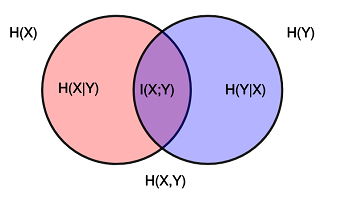
\includegraphics{https://raw.githubusercontent.com/ChristopheHunt/MSDA---Coursework/master/Data\%20605/Final\%20Project/Entropy-mutual-information-relative-entropy-relation-diagram.PNG}
{[}\^{}4{]}

{[}\^{}4{]} By KonradVoelkel (Own work) {[}Public domain{]}, via
Wikimedia Commons

\section{Descriptive and Inferential
Statistics.}\label{descriptive-and-inferential-statistics.}

Provide univariate descriptive statistics and appropriate plots for both
variables.

\begin{Shaded}
\begin{Highlighting}[]
\NormalTok{description <-}\StringTok{ }\KeywordTok{describe}\NormalTok{(sub.train.df[}\StringTok{"LotArea"}\NormalTok{])}
\KeywordTok{latex}\NormalTok{(description, }\DataTypeTok{file =} \StringTok{''}\NormalTok{)}
\end{Highlighting}
\end{Shaded}

\begin{spacing}{0.7}
\begin{center}\textbf{ sub.train.df["LotArea"] \\ 1 Variables~~~~~ 1460 ~Observations}\end{center}
\smallskip\hrule\smallskip{\small
\vbox{\noindent\textbf{LotArea}\setlength{\unitlength}{0.001in}\hfill\begin{picture}(1.5,.1)(1500,0)\linethickness{0.6pt}
\put(0,0){\line(0,1){15}}
\put(14,0){\line(0,1){25}}
\put(27,0){\line(0,1){34}}
\put(41,0){\line(0,1){97}}
\put(54,0){\line(0,1){100}}
\put(68,0){\line(0,1){58}}
\put(81,0){\line(0,1){29}}
\put(95,0){\line(0,1){11}}
\put(108,0){\line(0,1){6}}
\put(122,0){\line(0,1){3}}
\put(135,0){\line(0,1){3}}
\put(149,0){\line(0,1){1}}
\put(162,0){\line(0,1){2}}
\put(176,0){\line(0,1){1}}
\put(189,0){\line(0,1){1}}
\put(203,0){\line(0,1){1}}
\put(217,0){\line(0,1){1}}
\put(230,0){\line(0,1){1}}
\put(257,0){\line(0,1){1}}
\put(298,0){\line(0,1){1}}
\put(325,0){\line(0,1){1}}
\put(352,0){\line(0,1){1}}
\put(379,0){\line(0,1){1}}
\put(420,0){\line(0,1){1}}
\put(460,0){\line(0,1){1}}
\put(772,0){\line(0,1){1}}
\put(1069,0){\line(0,1){1}}
\put(1096,0){\line(0,1){1}}
\put(1448,0){\line(0,1){1}}
\end{picture}

{\smaller
\begin{tabular}{ rrrrrrrrrrrrr }
n&missing&distinct&Info&Mean&Gmd&.05&.10&.25&.50&.75&.90&.95 \\
1460&0&1073&1&10517&5718& 3312& 5000& 7554& 9478&11602&14382&17401 \end{tabular}
\begin{verbatim}

lowest :   1300   1477   1491   1526   1533, highest:  70761 115149 159000 164660 215245
\end{verbatim}
}
\smallskip\hrule\smallskip
}
}\end{spacing}

\begin{quote}
The histogram in the upper right corner of the table shows a right
skewed distribution, which is not surprising since houses in cities
would likely have similar relatively smaller lot areas versus instances
of large lot areas.
\end{quote}

\begin{Shaded}
\begin{Highlighting}[]
\NormalTok{description <-}\StringTok{ }\KeywordTok{describe}\NormalTok{(sub.train.df[}\StringTok{"SalePrice"}\NormalTok{])}
\KeywordTok{latex}\NormalTok{(description, }\DataTypeTok{file =} \StringTok{''}\NormalTok{)}
\end{Highlighting}
\end{Shaded}

\begin{spacing}{0.7}
\begin{center}\textbf{ sub.train.df["SalePrice"] \\ 1 Variables~~~~~ 1460 ~Observations}\end{center}
\smallskip\hrule\smallskip{\small
\vbox{\noindent\textbf{SalePrice}\setlength{\unitlength}{0.001in}\hfill\begin{picture}(1.5,.1)(1500,0)\linethickness{0.6pt}
\put(0,0){\line(0,1){1}}
\put(20,0){\line(0,1){3}}
\put(41,0){\line(0,1){3}}
\put(61,0){\line(0,1){6}}
\put(82,0){\line(0,1){6}}
\put(102,0){\line(0,1){24}}
\put(123,0){\line(0,1){32}}
\put(143,0){\line(0,1){25}}
\put(164,0){\line(0,1){64}}
\put(184,0){\line(0,1){58}}
\put(204,0){\line(0,1){100}}
\put(225,0){\line(0,1){89}}
\put(245,0){\line(0,1){80}}
\put(266,0){\line(0,1){57}}
\put(286,0){\line(0,1){68}}
\put(307,0){\line(0,1){64}}
\put(327,0){\line(0,1){61}}
\put(347,0){\line(0,1){35}}
\put(368,0){\line(0,1){40}}
\put(388,0){\line(0,1){24}}
\put(409,0){\line(0,1){36}}
\put(429,0){\line(0,1){26}}
\put(450,0){\line(0,1){20}}
\put(470,0){\line(0,1){19}}
\put(491,0){\line(0,1){21}}
\put(511,0){\line(0,1){13}}
\put(531,0){\line(0,1){12}}
\put(552,0){\line(0,1){6}}
\put(572,0){\line(0,1){12}}
\put(593,0){\line(0,1){10}}
\put(613,0){\line(0,1){10}}
\put(634,0){\line(0,1){6}}
\put(654,0){\line(0,1){4}}
\put(675,0){\line(0,1){2}}
\put(695,0){\line(0,1){5}}
\put(715,0){\line(0,1){4}}
\put(736,0){\line(0,1){6}}
\put(756,0){\line(0,1){3}}
\put(777,0){\line(0,1){1}}
\put(797,0){\line(0,1){2}}
\put(818,0){\line(0,1){1}}
\put(838,0){\line(0,1){2}}
\put(858,0){\line(0,1){1}}
\put(899,0){\line(0,1){2}}
\put(940,0){\line(0,1){1}}
\put(961,0){\line(0,1){1}}
\put(1042,0){\line(0,1){1}}
\put(1063,0){\line(0,1){1}}
\put(1083,0){\line(0,1){1}}
\put(1124,0){\line(0,1){1}}
\put(1186,0){\line(0,1){1}}
\put(1226,0){\line(0,1){1}}
\put(1472,0){\line(0,1){1}}
\end{picture}

{\smaller[2]
\begin{tabular}{ rrrrrrrrrrrrr }
n&missing&distinct&Info&Mean&Gmd&.05&.10&.25&.50&.75&.90&.95 \\
1460&0&663&1&180921&81086& 88000&106475&129975&163000&214000&278000&326100 \end{tabular}
\begin{verbatim}

lowest :  34900  35311  37900  39300  40000, highest: 582933 611657 625000 745000 755000
\end{verbatim}
}
\smallskip\hrule\smallskip
}
}\end{spacing}

\begin{quote}
As we can see from the histogram the shape of the data is near normal.
It is interesting to visualize that lot area does not follow the same
shape, this would hold with our original assumption that where the house
is located has more impact than the size of the lot area.
\end{quote}

Provide a scatterplot of X and Y.

\begin{Shaded}
\begin{Highlighting}[]
\KeywordTok{ggplot}\NormalTok{(sub.train.df, }\KeywordTok{aes}\NormalTok{(}\DataTypeTok{x =} \NormalTok{LotArea, }\DataTypeTok{y =} \NormalTok{SalePrice)) +}\StringTok{ }\KeywordTok{geom_point}\NormalTok{(}\DataTypeTok{shape =} \DecValTok{1}\NormalTok{) +}\StringTok{ }
\StringTok{    }\KeywordTok{theme_light}\NormalTok{() +}\StringTok{ }\KeywordTok{scale_y_continuous}\NormalTok{(}\DataTypeTok{labels =} \NormalTok{dollar)}
\end{Highlighting}
\end{Shaded}

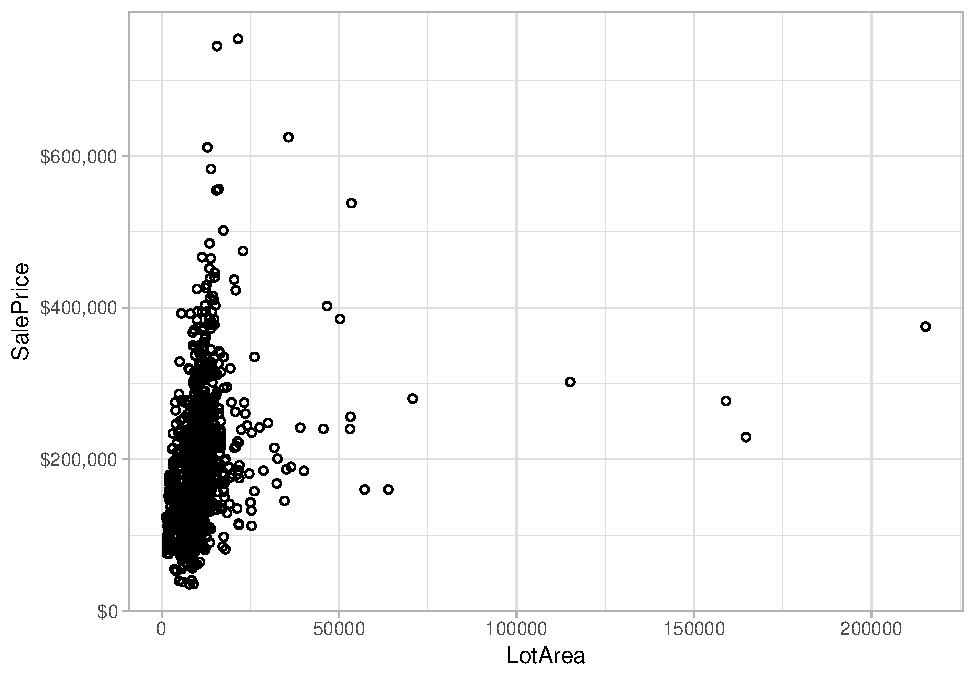
\includegraphics{Final_Project_files/figure-latex/scatter plot-1.pdf}

Transform both variables simultaneously using Box-Cox transformations.

\begin{quote}
I am using the \texttt{BoxCox.lambda} function from the
\texttt{forecast} package to determine the necessary transformations for
the two variables.
\end{quote}

\begin{Shaded}
\begin{Highlighting}[]
\KeywordTok{library}\NormalTok{(forecast)}
\KeywordTok{library}\NormalTok{(knitr)}
\NormalTok{l1 <-}\StringTok{ }\KeywordTok{BoxCox.lambda}\NormalTok{(}\KeywordTok{as.numeric}\NormalTok{(sub.train.df$SalePrice))}
\NormalTok{l2 <-}\StringTok{ }\KeywordTok{BoxCox.lambda}\NormalTok{(}\KeywordTok{as.numeric}\NormalTok{(sub.train.df$LotArea))}

\NormalTok{lamdas <-}\StringTok{ }\KeywordTok{c}\NormalTok{(l1, l2)}
\NormalTok{Variables <-}\StringTok{ }\KeywordTok{c}\NormalTok{(}\StringTok{"SalePrice"}\NormalTok{, }\StringTok{"LotArea"}\NormalTok{)}
\NormalTok{dfBoxCox <-}\StringTok{ }\KeywordTok{as.data.frame}\NormalTok{(}\KeywordTok{cbind}\NormalTok{(}\KeywordTok{round}\NormalTok{(}\KeywordTok{as.numeric}\NormalTok{(lamdas),}\DecValTok{4}\NormalTok{), Variables))}
\KeywordTok{colnames}\NormalTok{(dfBoxCox) <-}\StringTok{ }\KeywordTok{c}\NormalTok{(}\StringTok{"$}\CharTok{\textbackslash{}\textbackslash{}}\StringTok{lambda$"}\NormalTok{, }\StringTok{"Variables"}\NormalTok{)}
\KeywordTok{kable}\NormalTok{(dfBoxCox, }\DataTypeTok{align =} \KeywordTok{c}\NormalTok{(}\StringTok{"c"}\NormalTok{, }\StringTok{"c"}\NormalTok{))}
\end{Highlighting}
\end{Shaded}

\begin{longtable}[]{@{}cc@{}}
\toprule
\(\lambda\) & Variables\tabularnewline
\midrule
\endhead
-0.3308 & SalePrice\tabularnewline
-0.1268 & LotArea\tabularnewline
\bottomrule
\end{longtable}

\centering

Common Box-Cox Transformations\footnote{Osborne, Jason W. ``Improving
  your data transformations: Applying the Box-Cox transformation.''
  Practical Assessment, Research \& Evaluation 15.12 (2010): 1-9.}
\footnote{\href{https://www.isixsigma.com/tools-templates/normality/making-data-normal-using-box-cox-power-transformation/}{By
  Understanding Both the Concept of Transformation and the Box-Cox
  Method, Practitioners Will Be Better Prepared to Work with Non-normal
  Data.} . ``Making Data Normal Using Box-Cox Power Transformation.''
  ISixSigma. N.p., n.d. Web. 29 Oct. 2016.}

\setlength{\tabcolsep}{12pt}

\begin{tabular}{ c c }
\hline
$\lambda$ & Y' \\ \hline
-0.5 &  $Y^{-0.5}~=~\frac{1}{\sqrt{(Y)}}$ \\
0   & $\log(Y)$ \\
.25  & $\sqrt[4]{Y}$
\end{tabular}

\justifying

Lambda values were truncated to the nearest tenth that match a common
transformation as per the below table.

\centering

\begin{tabular}{ c c }
\hline
variable & variable transformation \\ \hline
SalePrice & $SalePrice^{-0.5}$ \\
LotArea & $log(LotArea)$ 
\end{tabular}

\justifying

\setlength{\tabcolsep}{6pt}

\subsection{Correlation Analysis}\label{correlation-analysis}

Using the transformed variables, run a correlation analysis and
interpret.

\begin{Shaded}
\begin{Highlighting}[]
\NormalTok{sub.train.df.trans <-}\StringTok{ }\NormalTok{sub.train.df %>%}\StringTok{ }
\StringTok{                      }\KeywordTok{mutate}\NormalTok{(}\DataTypeTok{SalePrice =} \NormalTok{SalePrice^(-.}\DecValTok{5}\NormalTok{), }
                             \DataTypeTok{LotArea =} \KeywordTok{log}\NormalTok{(LotArea))}

\NormalTok{sub.train.cor <-}\StringTok{ }\KeywordTok{cor.test}\NormalTok{(sub.train.df.trans$SalePrice, }
                          \NormalTok{sub.train.df.trans$LotArea, }
                          \DataTypeTok{method =} \StringTok{"pearson"}\NormalTok{, }\DataTypeTok{conf.level =} \NormalTok{.}\DecValTok{99}\NormalTok{)}
\NormalTok{sub.train.cor}
\end{Highlighting}
\end{Shaded}

\begin{verbatim}
## 
##  Pearson's product-moment correlation
## 
## data:  sub.train.df.trans$SalePrice and sub.train.df.trans$LotArea
## t = -15.968, df = 1458, p-value < 2.2e-16
## alternative hypothesis: true correlation is not equal to 0
## 99 percent confidence interval:
##  -0.4417063 -0.3269282
## sample estimates:
##        cor 
## -0.3858091
\end{verbatim}

\begin{quote}
The p-value of the correlation test is 2.2e-16 which is less than the
significance level of alpha at .05. We are using the standard alpha as
there is no indication another any other value for alpha should be used.
We can therefore say that the log of lot size and sale price raised to
the -.5 power are significantly correlated with a negative correlation
coefficient of -0.386.
\end{quote}

Test the hypothesis that the correlation between these variables is 0
and provide a 99\% confidence interval.

\begin{quote}
The correlation test has specifically done that for us and we can safely
reject the null hypothesis as we see that our 99\% confidence interval
exists at the values (-0.441, -0.327) with a p-value \textless{}
2.2e-16.
\end{quote}

Discuss the meaning of your analysis.

\begin{quote}
This means two possible things could have occured, there is no
correlation and this data set is pulled from an unusual set of house
sales. Or, more likely with the values obtained, our assumption of 0
correlation is incorect and we have obtained a very typical data set and
must reject the null hypothesis because correlation does exist.
\end{quote}

\section{Linear Algebra and
Correlation.}\label{linear-algebra-and-correlation.}

\begin{Shaded}
\begin{Highlighting}[]
\NormalTok{A <-}\StringTok{ }\KeywordTok{cor}\NormalTok{(sub.train.df.trans)}
\KeywordTok{kable}\NormalTok{(A)}
\end{Highlighting}
\end{Shaded}

\begin{longtable}[]{@{}lrr@{}}
\toprule
& SalePrice & LotArea\tabularnewline
\midrule
\endhead
SalePrice & 1.0000000 & -0.3858091\tabularnewline
LotArea & -0.3858091 & 1.0000000\tabularnewline
\bottomrule
\end{longtable}

Invert your correlation matrix.(This is known as the precision matrix
and contains variance inflation factors on the diagonal.)

\begin{Shaded}
\begin{Highlighting}[]
\NormalTok{B <-}\StringTok{ }\KeywordTok{solve}\NormalTok{(A)}
\KeywordTok{kable}\NormalTok{(B)}
\end{Highlighting}
\end{Shaded}

\begin{longtable}[]{@{}lrr@{}}
\toprule
& SalePrice & LotArea\tabularnewline
\midrule
\endhead
SalePrice & 1.1748792 & 0.4532792\tabularnewline
LotArea & 0.4532792 & 1.1748792\tabularnewline
\bottomrule
\end{longtable}

Multiply the correlation matrix by the precision matrix, and then
multiply the precision matrix by the correlation matrix.

\begin{Shaded}
\begin{Highlighting}[]
\NormalTok{corr.by.pre.M <-}\StringTok{ }\NormalTok{A %*%}\StringTok{ }\NormalTok{B}
\KeywordTok{kable}\NormalTok{(corr.by.pre.M)}
\end{Highlighting}
\end{Shaded}

\begin{longtable}[]{@{}lrr@{}}
\toprule
& SalePrice & LotArea\tabularnewline
\midrule
\endhead
SalePrice & 1 & 0\tabularnewline
LotArea & 0 & 1\tabularnewline
\bottomrule
\end{longtable}

\begin{Shaded}
\begin{Highlighting}[]
\NormalTok{pre.by.corr.M <-}\StringTok{ }\NormalTok{B %*%}\StringTok{ }\NormalTok{A}
\KeywordTok{kable}\NormalTok{(pre.by.corr.M)}
\end{Highlighting}
\end{Shaded}

\begin{longtable}[]{@{}lrr@{}}
\toprule
& SalePrice & LotArea\tabularnewline
\midrule
\endhead
SalePrice & 1 & 0\tabularnewline
LotArea & 0 & 1\tabularnewline
\bottomrule
\end{longtable}

\section{Calculus-Based Probability \&
Statistics}\label{calculus-based-probability-statistics}

Many times, it makes sense to fit a closed form distribution to data.
For your non-transformed independent variable, location shift it so that
the minimum value is above zero.

\begin{Shaded}
\begin{Highlighting}[]
\KeywordTok{min}\NormalTok{(sub.train.df$LotArea)}
\end{Highlighting}
\end{Shaded}

{[}1{]} 1300

\begin{quote}
For the independent variable chosen, there are no zero values observed.
This makes sense as we would expect the lot area to have some value and
I would expect it to never be unobserved (an assumption that at least
estimates would be used without a true figure).
\end{quote}

\begin{quote}
However, if a shift was required something like the below could be used.
\end{quote}

\begin{Shaded}
\begin{Highlighting}[]
\NormalTok{shift <-}\StringTok{ }\NormalTok{sub.train.df$LotArea +}\StringTok{ }\DecValTok{1} 
\end{Highlighting}
\end{Shaded}

Then load the MASS package and run fitdistr to fit a density function of
your choice. (See
\url{https://stat.ethz.ch/R-manual/R-devel/library/MASS/html/fitdistr.html}).

\begin{quote}
First lets look at what distrubtion would best fit our data.
\end{quote}

\begin{Shaded}
\begin{Highlighting}[]
\KeywordTok{library}\NormalTok{(fitdistrplus)}
\KeywordTok{descdist}\NormalTok{(sub.train.df$LotArea, }\DataTypeTok{discrete=}\OtherTok{FALSE}\NormalTok{, }\DataTypeTok{boot=}\DecValTok{500}\NormalTok{)}
\end{Highlighting}
\end{Shaded}

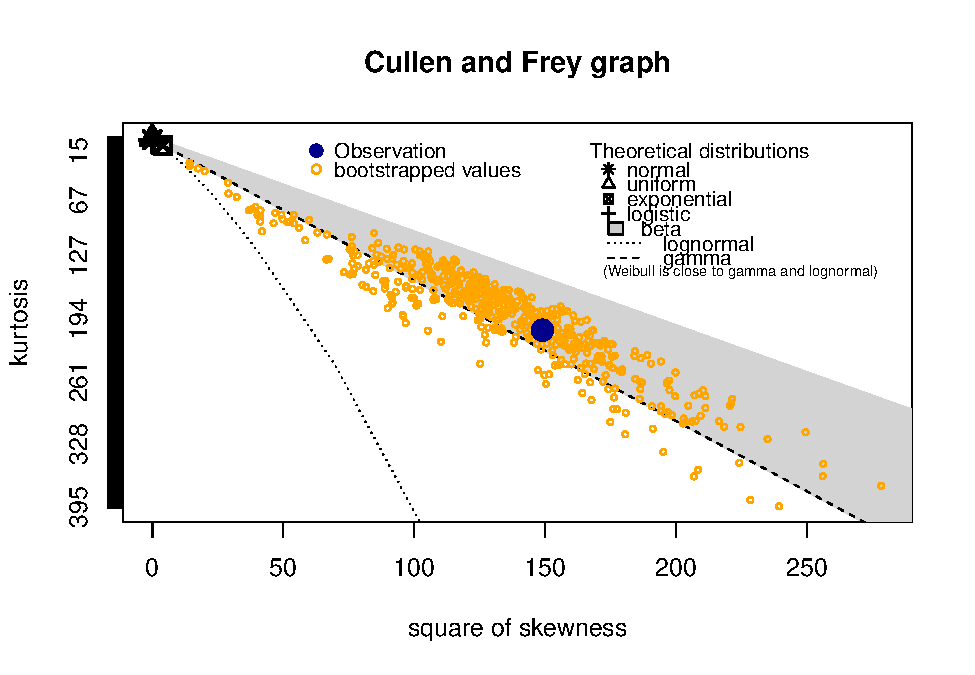
\includegraphics{Final_Project_files/figure-latex/unnamed-chunk-14-1.pdf}

\begin{verbatim}
## summary statistics
## ------
## min:  1300   max:  215245 
## median:  9478.5 
## mean:  10516.83 
## estimated sd:  9981.265 
## estimated skewness:  12.20769 
## estimated kurtosis:  206.2433
\end{verbatim}

\begin{quote}
There were too many issues in attempting to fit the beta distribution so
the next best theoretical distribution was used - log normal.
\end{quote}

\begin{Shaded}
\begin{Highlighting}[]
\KeywordTok{library}\NormalTok{(MASS)}
\NormalTok{fit.log <-}\StringTok{ }\KeywordTok{fitdistr}\NormalTok{(sub.train.df$LotArea, }\DataTypeTok{densfun =} \StringTok{"log-normal"}\NormalTok{)}
\NormalTok{fit.log}
\end{Highlighting}
\end{Shaded}

\begin{verbatim}
##      meanlog        sdlog   
##   9.110838240   0.517270830 
##  (0.013537596) (0.009572526)
\end{verbatim}

\begin{Shaded}
\begin{Highlighting}[]
\KeywordTok{hist}\NormalTok{(}\KeywordTok{log}\NormalTok{(sub.train.df$LotArea), }\DataTypeTok{prob=}\OtherTok{TRUE}\NormalTok{, }\DataTypeTok{xlab =} \StringTok{"Log of Lot Area"}\NormalTok{, }\DataTypeTok{main =} \StringTok{""}\NormalTok{)}
\KeywordTok{curve}\NormalTok{(}\KeywordTok{dnorm}\NormalTok{(x, fit.log$estimate[}\DecValTok{1}\NormalTok{], fit.log$estimate[}\DecValTok{2}\NormalTok{]), }\DataTypeTok{col=}\StringTok{"red"}\NormalTok{, }\DataTypeTok{lwd=}\DecValTok{2}\NormalTok{, }\DataTypeTok{add=}\NormalTok{T)}
\end{Highlighting}
\end{Shaded}

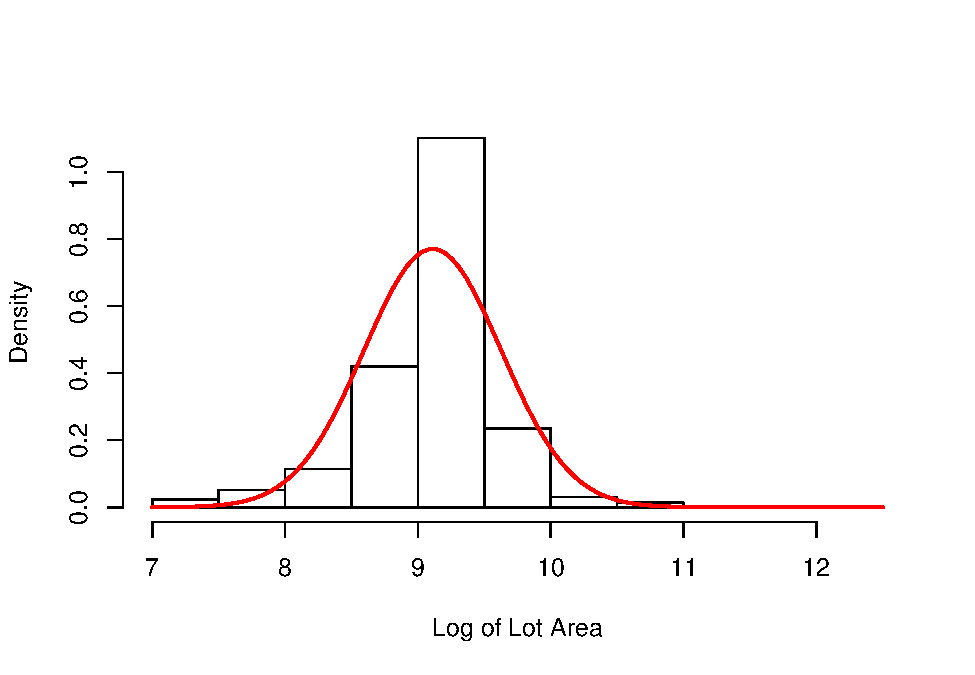
\includegraphics{Final_Project_files/figure-latex/unnamed-chunk-16-1.pdf}

\begin{quote}
From our density plot, the distribution looks quite good.
\end{quote}

Find the optimal value of the parameters for this distribution, and then
take 1000 samples from this distribution (e.g., rexp(1000) for an
exponential).

\begin{Shaded}
\begin{Highlighting}[]
\KeywordTok{set.seed}\NormalTok{(}\DecValTok{1234}\NormalTok{)}
\NormalTok{sample <-}\StringTok{ }\KeywordTok{rlnorm}\NormalTok{(}\DecValTok{1000}\NormalTok{, }\DataTypeTok{meanlog =} \NormalTok{fit.log$estimate[}\DecValTok{1}\NormalTok{], }\DataTypeTok{sdlog =} \NormalTok{fit.log$estimate[}\DecValTok{2}\NormalTok{])}
\end{Highlighting}
\end{Shaded}

Plot a histogram and compare it with a histogram of your non-transformed
original variable.

\begin{Shaded}
\begin{Highlighting}[]
\KeywordTok{hist}\NormalTok{(sample, }\DataTypeTok{pch =} \DecValTok{20}\NormalTok{, }\DataTypeTok{breaks =} \DecValTok{25}\NormalTok{, }\DataTypeTok{col =} \KeywordTok{rgb}\NormalTok{(}\DecValTok{1}\NormalTok{,}\DecValTok{0}\NormalTok{,}\DecValTok{0}\NormalTok{,}\FloatTok{0.5}\NormalTok{), }\DataTypeTok{xlim =} \KeywordTok{c}\NormalTok{(}\DecValTok{0}\NormalTok{,}\DecValTok{50000}\NormalTok{), }\DataTypeTok{ylim =} \KeywordTok{c}\NormalTok{(}\DecValTok{0}\NormalTok{,}\DecValTok{500}\NormalTok{), }\DataTypeTok{main =} \StringTok{'Overlapping Histogram'}\NormalTok{, }\DataTypeTok{xlab =} \StringTok{'Variable'}\NormalTok{) }
\KeywordTok{hist}\NormalTok{(sub.train.df$LotArea, }\DataTypeTok{pch =} \DecValTok{20}\NormalTok{, }\DataTypeTok{breaks =} \DecValTok{100}\NormalTok{, }\DataTypeTok{col =} \KeywordTok{rgb}\NormalTok{(}\DecValTok{0}\NormalTok{,}\DecValTok{0}\NormalTok{,}\DecValTok{1}\NormalTok{,}\FloatTok{0.5}\NormalTok{), }\DataTypeTok{add =} \NormalTok{T) }
\CommentTok{#https://www.r-bloggers.com/overlapping-histogram-in-r/}
\KeywordTok{legend}\NormalTok{(}\StringTok{"topright"}\NormalTok{, }\KeywordTok{c}\NormalTok{(}\StringTok{"Sample"}\NormalTok{, }\StringTok{"Actual"}\NormalTok{), }\DataTypeTok{col=}\KeywordTok{c}\NormalTok{(}\KeywordTok{rgb}\NormalTok{(}\DecValTok{1}\NormalTok{,}\DecValTok{0}\NormalTok{,}\DecValTok{0}\NormalTok{,}\FloatTok{0.5}\NormalTok{), }\KeywordTok{rgb}\NormalTok{(}\DecValTok{0}\NormalTok{,}\DecValTok{0}\NormalTok{,}\DecValTok{1}\NormalTok{,}\FloatTok{0.5}\NormalTok{)), }\DataTypeTok{lwd=}\DecValTok{10}\NormalTok{)}
\end{Highlighting}
\end{Shaded}

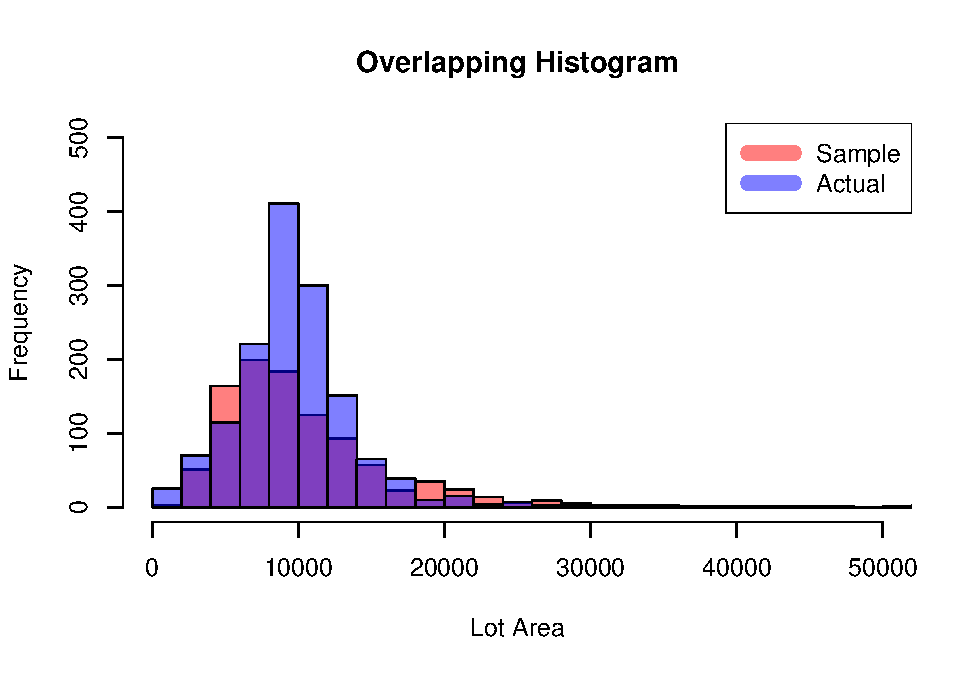
\includegraphics{Final_Project_files/figure-latex/unnamed-chunk-18-1.pdf}

\begin{quote}
It is clear that the distributions are very similar. Plotting them
overlapping gives a clear visual of how similar the distributions, note
that x has been limited and does not extend out for extreme values of x.
\end{quote}

\section{Modeling}\label{modeling}

Build some type of regression model and submit your model to the
competition board.

\begin{Shaded}
\begin{Highlighting}[]
\NormalTok{description <-}\StringTok{ }\KeywordTok{describe}\NormalTok{(train.df %>%}\StringTok{ }\NormalTok{dplyr::}\KeywordTok{select}\NormalTok{(-Id, -SalePrice))}
\KeywordTok{latex}\NormalTok{(description, }\DataTypeTok{file =} \StringTok{''}\NormalTok{)}
\end{Highlighting}
\end{Shaded}

\begin{spacing}{0.7}
\begin{center}\textbf{ train.df \%$>$\% dplyr::select(-Id, -SalePrice) \\ 79 Variables~~~~~ 1460 ~Observations}\end{center}
\smallskip\hrule\smallskip{\small
\vbox{\noindent\textbf{MSSubClass}\setlength{\unitlength}{0.001in}\hfill\begin{picture}(1.5,.1)(1500,0)\linethickness{0.6pt}
\put(0,0){\line(0,1){100}}
\put(82,0){\line(0,1){13}}
\put(165,0){\line(0,1){1}}
\put(206,0){\line(0,1){2}}
\put(247,0){\line(0,1){27}}
\put(329,0){\line(0,1){56}}
\put(412,0){\line(0,1){11}}
\put(453,0){\line(0,1){3}}
\put(494,0){\line(0,1){11}}
\put(535,0){\line(0,1){4}}
\put(576,0){\line(0,1){10}}
\put(824,0){\line(0,1){16}}
\put(1153,0){\line(0,1){12}}
\put(1318,0){\line(0,1){2}}
\put(1400,0){\line(0,1){6}}
\end{picture}

{\smaller
\begin{tabular}{ rrrrrrrrrrrrr }
n&missing&distinct&Info&Mean&Gmd&.05&.10&.25&.50&.75&.90&.95 \\
1460&0&15&0.94&56.9&43.19& 20& 20& 20& 50& 70&120&160 \end{tabular}
\begin{verbatim}
                                                                                              
Value         20    30    40    45    50    60    70    75    80    85    90   120   160   180
Frequency    536    69     4    12   144   299    60    16    58    20    52    87    63    10
Proportion 0.367 0.047 0.003 0.008 0.099 0.205 0.041 0.011 0.040 0.014 0.036 0.060 0.043 0.007
                
Value        190
Frequency     30
Proportion 0.021
\end{verbatim}
}
\smallskip\hrule\smallskip
}
\vbox{\noindent\textbf{MSZoning}\setlength{\unitlength}{0.001in}\hfill\begin{picture}(1.5,.1)(1500,0)\linethickness{0.6pt}
\put(0,0){\line(0,1){1}}
\put(300,0){\line(0,1){6}}
\put(600,0){\line(0,1){1}}
\put(900,0){\line(0,1){100}}
\put(1200,0){\line(0,1){19}}
\end{picture}

{\smaller
\begin{tabular}{ rrr }
n&missing&distinct \\
1460&0&5 \end{tabular}
\begin{verbatim}
                                                  
Value      C (all)      FV      RH      RL      RM
Frequency       10      65      16    1151     218
Proportion   0.007   0.045   0.011   0.788   0.149
\end{verbatim}
}
\smallskip\hrule\smallskip
}
\vbox{\noindent\textbf{LotFrontage}\setlength{\unitlength}{0.001in}\hfill\begin{picture}(1.5,.1)(1500,0)\linethickness{0.6pt}
\put(0,0){\line(0,1){13}}
\put(25,0){\line(0,1){11}}
\put(49,0){\line(0,1){6}}
\put(74,0){\line(0,1){17}}
\put(99,0){\line(0,1){13}}
\put(123,0){\line(0,1){17}}
\put(148,0){\line(0,1){53}}
\put(173,0){\line(0,1){28}}
\put(197,0){\line(0,1){100}}
\put(222,0){\line(0,1){59}}
\put(247,0){\line(0,1){72}}
\put(271,0){\line(0,1){59}}
\put(296,0){\line(0,1){72}}
\put(320,0){\line(0,1){38}}
\put(345,0){\line(0,1){31}}
\put(370,0){\line(0,1){17}}
\put(394,0){\line(0,1){18}}
\put(419,0){\line(0,1){11}}
\put(444,0){\line(0,1){7}}
\put(468,0){\line(0,1){3}}
\put(493,0){\line(0,1){7}}
\put(518,0){\line(0,1){1}}
\put(542,0){\line(0,1){3}}
\put(567,0){\line(0,1){2}}
\put(592,0){\line(0,1){2}}
\put(616,0){\line(0,1){1}}
\put(641,0){\line(0,1){2}}
\put(666,0){\line(0,1){1}}
\put(690,0){\line(0,1){1}}
\put(740,0){\line(0,1){1}}
\put(764,0){\line(0,1){1}}
\put(789,0){\line(0,1){1}}
\put(1455,0){\line(0,1){1}}
\end{picture}

{\smaller
\begin{tabular}{ rrrrrrrrrrrrr }
n&missing&distinct&Info&Mean&Gmd&.05&.10&.25&.50&.75&.90&.95 \\
1201&259&110&0.998&70.05&24.61& 34& 44& 59& 69& 80& 96&107 \end{tabular}
\begin{verbatim}

lowest :  21  24  30  32  33, highest: 160 168 174 182 313
\end{verbatim}
}
\smallskip\hrule\smallskip
}
\vbox{\noindent\textbf{LotArea}\setlength{\unitlength}{0.001in}\hfill\begin{picture}(1.5,.1)(1500,0)\linethickness{0.6pt}
\put(0,0){\line(0,1){15}}
\put(14,0){\line(0,1){25}}
\put(27,0){\line(0,1){34}}
\put(41,0){\line(0,1){97}}
\put(54,0){\line(0,1){100}}
\put(68,0){\line(0,1){58}}
\put(81,0){\line(0,1){29}}
\put(95,0){\line(0,1){11}}
\put(108,0){\line(0,1){6}}
\put(122,0){\line(0,1){3}}
\put(135,0){\line(0,1){3}}
\put(149,0){\line(0,1){1}}
\put(162,0){\line(0,1){2}}
\put(176,0){\line(0,1){1}}
\put(189,0){\line(0,1){1}}
\put(203,0){\line(0,1){1}}
\put(217,0){\line(0,1){1}}
\put(230,0){\line(0,1){1}}
\put(257,0){\line(0,1){1}}
\put(298,0){\line(0,1){1}}
\put(325,0){\line(0,1){1}}
\put(352,0){\line(0,1){1}}
\put(379,0){\line(0,1){1}}
\put(420,0){\line(0,1){1}}
\put(460,0){\line(0,1){1}}
\put(772,0){\line(0,1){1}}
\put(1069,0){\line(0,1){1}}
\put(1096,0){\line(0,1){1}}
\put(1448,0){\line(0,1){1}}
\end{picture}

{\smaller
\begin{tabular}{ rrrrrrrrrrrrr }
n&missing&distinct&Info&Mean&Gmd&.05&.10&.25&.50&.75&.90&.95 \\
1460&0&1073&1&10517&5718& 3312& 5000& 7554& 9478&11602&14382&17401 \end{tabular}
\begin{verbatim}

lowest :   1300   1477   1491   1526   1533, highest:  70761 115149 159000 164660 215245
\end{verbatim}
}
\smallskip\hrule\smallskip
}
\vbox{\noindent\textbf{Street}

{\smaller
\begin{tabular}{ rrr }
n&missing&distinct \\
1460&0&2 \end{tabular}
\begin{verbatim}
                      
Value       Grvl  Pave
Frequency      6  1454
Proportion 0.004 0.996
\end{verbatim}
}
\smallskip\hrule\smallskip
}
\vbox{\noindent\textbf{Alley}

{\smaller
\begin{tabular}{ rrr }
n&missing&distinct \\
91&1369&2 \end{tabular}
\begin{verbatim}
                      
Value       Grvl  Pave
Frequency     50    41
Proportion 0.549 0.451
\end{verbatim}
}
\smallskip\hrule\smallskip
}
\vbox{\noindent\textbf{LotShape}\setlength{\unitlength}{0.001in}\hfill\begin{picture}(1.5,.1)(1500,0)\linethickness{0.6pt}
\put(0,0){\line(0,1){52}}
\put(375,0){\line(0,1){4}}
\put(750,0){\line(0,1){1}}
\put(1125,0){\line(0,1){100}}
\end{picture}

{\smaller
\begin{tabular}{ rrr }
n&missing&distinct \\
1460&0&4 \end{tabular}
\begin{verbatim}
                                  
Value        IR1   IR2   IR3   Reg
Frequency    484    41    10   925
Proportion 0.332 0.028 0.007 0.634
\end{verbatim}
}
\smallskip\hrule\smallskip
}
\vbox{\noindent\textbf{LandContour}\setlength{\unitlength}{0.001in}\hfill\begin{picture}(1.5,.1)(1500,0)\linethickness{0.6pt}
\put(0,0){\line(0,1){5}}
\put(375,0){\line(0,1){4}}
\put(750,0){\line(0,1){3}}
\put(1125,0){\line(0,1){100}}
\end{picture}

{\smaller
\begin{tabular}{ rrr }
n&missing&distinct \\
1460&0&4 \end{tabular}
\begin{verbatim}
                                  
Value        Bnk   HLS   Low   Lvl
Frequency     63    50    36  1311
Proportion 0.043 0.034 0.025 0.898
\end{verbatim}
}
\smallskip\hrule\smallskip
}
\vbox{\noindent\textbf{Utilities}

{\smaller
\begin{tabular}{ rrr }
n&missing&distinct \\
1460&0&2 \end{tabular}
\begin{verbatim}
                        
Value      AllPub NoSeWa
Frequency    1459      1
Proportion  0.999  0.001
\end{verbatim}
}
\smallskip\hrule\smallskip
}
\vbox{\noindent\textbf{LotConfig}\setlength{\unitlength}{0.001in}\hfill\begin{picture}(1.5,.1)(1500,0)\linethickness{0.6pt}
\put(0,0){\line(0,1){25}}
\put(300,0){\line(0,1){9}}
\put(600,0){\line(0,1){4}}
\put(900,0){\line(0,1){1}}
\put(1200,0){\line(0,1){100}}
\end{picture}

{\smaller
\begin{tabular}{ rrr }
n&missing&distinct \\
1460&0&5 \end{tabular}
\begin{verbatim}
                                                  
Value       Corner CulDSac     FR2     FR3  Inside
Frequency      263      94      47       4    1052
Proportion   0.180   0.064   0.032   0.003   0.721
\end{verbatim}
}
\smallskip\hrule\smallskip
}
\vbox{\noindent\textbf{LandSlope}\setlength{\unitlength}{0.001in}\hfill\begin{picture}(1.5,.1)(1500,0)\linethickness{0.6pt}
\put(0,0){\line(0,1){100}}
\put(500,0){\line(0,1){5}}
\put(1000,0){\line(0,1){1}}
\end{picture}

{\smaller
\begin{tabular}{ rrr }
n&missing&distinct \\
1460&0&3 \end{tabular}
\begin{verbatim}
                            
Value        Gtl   Mod   Sev
Frequency   1382    65    13
Proportion 0.947 0.045 0.009
\end{verbatim}
}
\smallskip\hrule\smallskip
}
\vbox{\noindent\textbf{Neighborhood}\setlength{\unitlength}{0.001in}\hfill\begin{picture}(1.5,.1)(1500,0)\linethickness{0.6pt}
\put(0,0){\line(0,1){8}}
\put(60,0){\line(0,1){1}}
\put(120,0){\line(0,1){7}}
\put(180,0){\line(0,1){26}}
\put(240,0){\line(0,1){12}}
\put(300,0){\line(0,1){67}}
\put(360,0){\line(0,1){23}}
\put(420,0){\line(0,1){44}}
\put(480,0){\line(0,1){35}}
\put(540,0){\line(0,1){16}}
\put(600,0){\line(0,1){8}}
\put(660,0){\line(0,1){22}}
\put(720,0){\line(0,1){100}}
\put(780,0){\line(0,1){18}}
\put(840,0){\line(0,1){4}}
\put(900,0){\line(0,1){34}}
\put(960,0){\line(0,1){32}}
\put(1020,0){\line(0,1){50}}
\put(1080,0){\line(0,1){33}}
\put(1140,0){\line(0,1){26}}
\put(1200,0){\line(0,1){38}}
\put(1260,0){\line(0,1){11}}
\put(1320,0){\line(0,1){11}}
\put(1380,0){\line(0,1){17}}
\put(1440,0){\line(0,1){5}}
\end{picture}

{\smaller
\begin{tabular}{ rrr }
n&missing&distinct \\
1460&0&25 \end{tabular}
\begin{verbatim}

lowest : Blmngtn Blueste BrDale  BrkSide ClearCr, highest: Somerst StoneBr SWISU   Timber  Veenker
\end{verbatim}
}
\smallskip\hrule\smallskip
}
\vbox{\noindent\textbf{Condition1}\setlength{\unitlength}{0.001in}\hfill\begin{picture}(1.5,.1)(1500,0)\linethickness{0.6pt}
\put(0,0){\line(0,1){4}}
\put(167,0){\line(0,1){6}}
\put(333,0){\line(0,1){100}}
\put(500,0){\line(0,1){1}}
\put(667,0){\line(0,1){2}}
\put(833,0){\line(0,1){1}}
\put(1000,0){\line(0,1){2}}
\put(1167,0){\line(0,1){1}}
\put(1333,0){\line(0,1){1}}
\end{picture}

{\smaller
\begin{tabular}{ rrr }
n&missing&distinct \\
1460&0&9 \end{tabular}
\begin{verbatim}
                                                                         
Value      Artery  Feedr   Norm   PosA   PosN   RRAe   RRAn   RRNe   RRNn
Frequency      48     81   1260      8     19     11     26      2      5
Proportion  0.033  0.055  0.863  0.005  0.013  0.008  0.018  0.001  0.003
\end{verbatim}
}
\smallskip\hrule\smallskip
}
\vbox{\noindent\textbf{Condition2}\setlength{\unitlength}{0.001in}\hfill\begin{picture}(1.5,.1)(1500,0)\linethickness{0.6pt}
\put(0,0){\line(0,1){1}}
\put(188,0){\line(0,1){1}}
\put(375,0){\line(0,1){100}}
\put(562,0){\line(0,1){1}}
\put(750,0){\line(0,1){1}}
\put(938,0){\line(0,1){1}}
\put(1125,0){\line(0,1){1}}
\put(1312,0){\line(0,1){1}}
\end{picture}

{\smaller
\begin{tabular}{ rrr }
n&missing&distinct \\
1460&0&8 \end{tabular}
\begin{verbatim}
                                                                  
Value      Artery  Feedr   Norm   PosA   PosN   RRAe   RRAn   RRNn
Frequency       2      6   1445      1      2      1      1      2
Proportion  0.001  0.004  0.990  0.001  0.001  0.001  0.001  0.001
\end{verbatim}
}
\smallskip\hrule\smallskip
}
\vbox{\noindent\textbf{BldgType}\setlength{\unitlength}{0.001in}\hfill\begin{picture}(1.5,.1)(1500,0)\linethickness{0.6pt}
\put(0,0){\line(0,1){100}}
\put(300,0){\line(0,1){3}}
\put(600,0){\line(0,1){4}}
\put(900,0){\line(0,1){4}}
\put(1200,0){\line(0,1){9}}
\end{picture}

{\smaller
\begin{tabular}{ rrr }
n&missing&distinct \\
1460&0&5 \end{tabular}
\begin{verbatim}
                                             
Value        1Fam 2fmCon Duplex  Twnhs TwnhsE
Frequency    1220     31     52     43    114
Proportion  0.836  0.021  0.036  0.029  0.078
\end{verbatim}
}
\smallskip\hrule\smallskip
}
\vbox{\noindent\textbf{HouseStyle}\setlength{\unitlength}{0.001in}\hfill\begin{picture}(1.5,.1)(1500,0)\linethickness{0.6pt}
\put(0,0){\line(0,1){21}}
\put(188,0){\line(0,1){2}}
\put(375,0){\line(0,1){100}}
\put(562,0){\line(0,1){1}}
\put(750,0){\line(0,1){2}}
\put(938,0){\line(0,1){61}}
\put(1125,0){\line(0,1){5}}
\put(1312,0){\line(0,1){9}}
\end{picture}

{\smaller
\begin{tabular}{ rrr }
n&missing&distinct \\
1460&0&8 \end{tabular}
\begin{verbatim}
                                                                  
Value      1.5Fin 1.5Unf 1Story 2.5Fin 2.5Unf 2Story SFoyer   SLvl
Frequency     154     14    726      8     11    445     37     65
Proportion  0.105  0.010  0.497  0.005  0.008  0.305  0.025  0.045
\end{verbatim}
}
\smallskip\hrule\smallskip
}
\vbox{\noindent\textbf{OverallQual}\setlength{\unitlength}{0.001in}\hfill\begin{picture}(1.5,.1)(1500,0)\linethickness{0.6pt}
\put(0,0){\line(0,1){1}}
\put(150,0){\line(0,1){1}}
\put(300,0){\line(0,1){5}}
\put(450,0){\line(0,1){29}}
\put(600,0){\line(0,1){100}}
\put(750,0){\line(0,1){94}}
\put(900,0){\line(0,1){80}}
\put(1050,0){\line(0,1){42}}
\put(1200,0){\line(0,1){11}}
\put(1350,0){\line(0,1){5}}
\end{picture}

{\smaller
\begin{tabular}{ rrrrrrrrrrrrr }
n&missing&distinct&Info&Mean&Gmd&.05&.10&.25&.50&.75&.90&.95 \\
1460&0&10&0.951&6.099&1.522&4&5&5&6&7&8&8 \end{tabular}
\begin{verbatim}
                                                                      
Value          1     2     3     4     5     6     7     8     9    10
Frequency      2     3    20   116   397   374   319   168    43    18
Proportion 0.001 0.002 0.014 0.079 0.272 0.256 0.218 0.115 0.029 0.012
\end{verbatim}
}
\smallskip\hrule\smallskip
}
\vbox{\noindent\textbf{OverallCond}\setlength{\unitlength}{0.001in}\hfill\begin{picture}(1.5,.1)(1500,0)\linethickness{0.6pt}
\put(0,0){\line(0,1){1}}
\put(167,0){\line(0,1){1}}
\put(333,0){\line(0,1){3}}
\put(500,0){\line(0,1){7}}
\put(667,0){\line(0,1){100}}
\put(833,0){\line(0,1){31}}
\put(1000,0){\line(0,1){25}}
\put(1167,0){\line(0,1){9}}
\put(1333,0){\line(0,1){3}}
\end{picture}

{\smaller
\begin{tabular}{ rrrrrr }
n&missing&distinct&Info&Mean&Gmd \\
1460&0&9&0.814&5.575&1.111 \end{tabular}
\begin{verbatim}
                                                                
Value          1     2     3     4     5     6     7     8     9
Frequency      1     5    25    57   821   252   205    72    22
Proportion 0.001 0.003 0.017 0.039 0.562 0.173 0.140 0.049 0.015
\end{verbatim}
}
\smallskip\hrule\smallskip
}
\vbox{\noindent\textbf{YearBuilt}\setlength{\unitlength}{0.001in}\hfill\begin{picture}(1.5,.1)(1500,0)\linethickness{0.6pt}
\put(0,0){\line(0,1){1}}
\put(32,0){\line(0,1){1}}
\put(86,0){\line(0,1){6}}
\put(108,0){\line(0,1){1}}
\put(140,0){\line(0,1){3}}
\put(194,0){\line(0,1){3}}
\put(215,0){\line(0,1){3}}
\put(226,0){\line(0,1){1}}
\put(280,0){\line(0,1){1}}
\put(302,0){\line(0,1){15}}
\put(345,0){\line(0,1){1}}
\put(355,0){\line(0,1){1}}
\put(366,0){\line(0,1){1}}
\put(388,0){\line(0,1){3}}
\put(409,0){\line(0,1){25}}
\put(420,0){\line(0,1){1}}
\put(431,0){\line(0,1){4}}
\put(442,0){\line(0,1){1}}
\put(452,0){\line(0,1){10}}
\put(463,0){\line(0,1){15}}
\put(474,0){\line(0,1){12}}
\put(485,0){\line(0,1){1}}
\put(496,0){\line(0,1){10}}
\put(506,0){\line(0,1){4}}
\put(517,0){\line(0,1){45}}
\put(528,0){\line(0,1){9}}
\put(539,0){\line(0,1){12}}
\put(549,0){\line(0,1){10}}
\put(560,0){\line(0,1){10}}
\put(571,0){\line(0,1){24}}
\put(582,0){\line(0,1){13}}
\put(592,0){\line(0,1){4}}
\put(603,0){\line(0,1){10}}
\put(614,0){\line(0,1){6}}
\put(625,0){\line(0,1){13}}
\put(636,0){\line(0,1){9}}
\put(646,0){\line(0,1){6}}
\put(668,0){\line(0,1){4}}
\put(679,0){\line(0,1){9}}
\put(689,0){\line(0,1){13}}
\put(700,0){\line(0,1){7}}
\put(711,0){\line(0,1){6}}
\put(722,0){\line(0,1){12}}
\put(733,0){\line(0,1){27}}
\put(743,0){\line(0,1){22}}
\put(754,0){\line(0,1){3}}
\put(786,0){\line(0,1){9}}
\put(797,0){\line(0,1){10}}
\put(808,0){\line(0,1){7}}
\put(819,0){\line(0,1){21}}
\put(829,0){\line(0,1){18}}
\put(840,0){\line(0,1){30}}
\put(851,0){\line(0,1){9}}
\put(862,0){\line(0,1){7}}
\put(873,0){\line(0,1){18}}
\put(883,0){\line(0,1){36}}
\put(894,0){\line(0,1){24}}
\put(905,0){\line(0,1){21}}
\put(916,0){\line(0,1){30}}
\put(926,0){\line(0,1){36}}
\put(937,0){\line(0,1){39}}
\put(948,0){\line(0,1){25}}
\put(959,0){\line(0,1){21}}
\put(970,0){\line(0,1){28}}
\put(980,0){\line(0,1){24}}
\put(991,0){\line(0,1){22}}
\put(1002,0){\line(0,1){36}}
\put(1013,0){\line(0,1){27}}
\put(1023,0){\line(0,1){24}}
\put(1034,0){\line(0,1){33}}
\put(1045,0){\line(0,1){21}}
\put(1056,0){\line(0,1){36}}
\put(1066,0){\line(0,1){33}}
\put(1077,0){\line(0,1){34}}
\put(1088,0){\line(0,1){16}}
\put(1099,0){\line(0,1){15}}
\put(1110,0){\line(0,1){12}}
\put(1120,0){\line(0,1){49}}
\put(1131,0){\line(0,1){48}}
\put(1142,0){\line(0,1){24}}
\put(1153,0){\line(0,1){13}}
\put(1163,0){\line(0,1){15}}
\put(1174,0){\line(0,1){7}}
\put(1185,0){\line(0,1){9}}
\put(1196,0){\line(0,1){6}}
\put(1207,0){\line(0,1){13}}
\put(1217,0){\line(0,1){7}}
\put(1228,0){\line(0,1){7}}
\put(1239,0){\line(0,1){4}}
\put(1250,0){\line(0,1){16}}
\put(1260,0){\line(0,1){4}}
\put(1271,0){\line(0,1){18}}
\put(1282,0){\line(0,1){7}}
\put(1293,0){\line(0,1){19}}
\put(1303,0){\line(0,1){25}}
\put(1314,0){\line(0,1){28}}
\put(1325,0){\line(0,1){27}}
\put(1336,0){\line(0,1){22}}
\put(1347,0){\line(0,1){21}}
\put(1357,0){\line(0,1){37}}
\put(1368,0){\line(0,1){37}}
\put(1379,0){\line(0,1){36}}
\put(1390,0){\line(0,1){30}}
\put(1400,0){\line(0,1){34}}
\put(1411,0){\line(0,1){67}}
\put(1422,0){\line(0,1){81}}
\put(1433,0){\line(0,1){96}}
\put(1444,0){\line(0,1){100}}
\put(1454,0){\line(0,1){73}}
\put(1465,0){\line(0,1){34}}
\put(1476,0){\line(0,1){27}}
\put(1487,0){\line(0,1){1}}
\end{picture}

{\smaller
\begin{tabular}{ rrrrrrrrrrrrr }
n&missing&distinct&Info&Mean&Gmd&.05&.10&.25&.50&.75&.90&.95 \\
1460&0&112&1&1971&33.88&1916&1925&1954&1973&2000&2006&2007 \end{tabular}
\begin{verbatim}

lowest : 1872 1875 1880 1882 1885, highest: 2006 2007 2008 2009 2010
\end{verbatim}
}
\smallskip\hrule\smallskip
}
\vbox{\noindent\textbf{YearRemodAdd}\setlength{\unitlength}{0.001in}\hfill\begin{picture}(1.5,.1)(1500,0)\linethickness{0.6pt}
\put(0,0){\line(0,1){100}}
\put(25,0){\line(0,1){2}}
\put(49,0){\line(0,1){3}}
\put(74,0){\line(0,1){6}}
\put(98,0){\line(0,1){8}}
\put(123,0){\line(0,1){5}}
\put(148,0){\line(0,1){6}}
\put(172,0){\line(0,1){5}}
\put(197,0){\line(0,1){8}}
\put(221,0){\line(0,1){10}}
\put(246,0){\line(0,1){7}}
\put(270,0){\line(0,1){4}}
\put(295,0){\line(0,1){8}}
\put(320,0){\line(0,1){7}}
\put(344,0){\line(0,1){6}}
\put(369,0){\line(0,1){11}}
\put(393,0){\line(0,1){8}}
\put(418,0){\line(0,1){7}}
\put(443,0){\line(0,1){10}}
\put(467,0){\line(0,1){8}}
\put(492,0){\line(0,1){15}}
\put(516,0){\line(0,1){10}}
\put(541,0){\line(0,1){11}}
\put(566,0){\line(0,1){6}}
\put(590,0){\line(0,1){4}}
\put(615,0){\line(0,1){6}}
\put(639,0){\line(0,1){17}}
\put(664,0){\line(0,1){14}}
\put(689,0){\line(0,1){9}}
\put(713,0){\line(0,1){6}}
\put(738,0){\line(0,1){7}}
\put(762,0){\line(0,1){4}}
\put(787,0){\line(0,1){4}}
\put(811,0){\line(0,1){3}}
\put(836,0){\line(0,1){4}}
\put(861,0){\line(0,1){5}}
\put(885,0){\line(0,1){3}}
\put(910,0){\line(0,1){6}}
\put(934,0){\line(0,1){5}}
\put(959,0){\line(0,1){6}}
\put(984,0){\line(0,1){8}}
\put(1008,0){\line(0,1){8}}
\put(1033,0){\line(0,1){10}}
\put(1057,0){\line(0,1){11}}
\put(1082,0){\line(0,1){12}}
\put(1107,0){\line(0,1){17}}
\put(1131,0){\line(0,1){20}}
\put(1156,0){\line(0,1){14}}
\put(1180,0){\line(0,1){20}}
\put(1205,0){\line(0,1){17}}
\put(1230,0){\line(0,1){31}}
\put(1254,0){\line(0,1){12}}
\put(1279,0){\line(0,1){27}}
\put(1303,0){\line(0,1){29}}
\put(1328,0){\line(0,1){35}}
\put(1352,0){\line(0,1){41}}
\put(1377,0){\line(0,1){54}}
\put(1402,0){\line(0,1){43}}
\put(1426,0){\line(0,1){22}}
\put(1451,0){\line(0,1){13}}
\put(1475,0){\line(0,1){3}}
\end{picture}

{\smaller
\begin{tabular}{ rrrrrrrrrrrrr }
n&missing&distinct&Info&Mean&Gmd&.05&.10&.25&.50&.75&.90&.95 \\
1460&0&61&0.997&1985&23.05&1950&1950&1967&1994&2004&2006&2007 \end{tabular}
\begin{verbatim}

lowest : 1950 1951 1952 1953 1954, highest: 2006 2007 2008 2009 2010
\end{verbatim}
}
\smallskip\hrule\smallskip
}
\vbox{\noindent\textbf{RoofStyle}\setlength{\unitlength}{0.001in}\hfill\begin{picture}(1.5,.1)(1500,0)\linethickness{0.6pt}
\put(0,0){\line(0,1){1}}
\put(250,0){\line(0,1){100}}
\put(500,0){\line(0,1){1}}
\put(750,0){\line(0,1){25}}
\put(1000,0){\line(0,1){1}}
\put(1250,0){\line(0,1){1}}
\end{picture}

{\smaller
\begin{tabular}{ rrr }
n&missing&distinct \\
1460&0&6 \end{tabular}
\begin{verbatim}
                                                          
Value         Flat   Gable Gambrel     Hip Mansard    Shed
Frequency       13    1141      11     286       7       2
Proportion   0.009   0.782   0.008   0.196   0.005   0.001
\end{verbatim}
}
\smallskip\hrule\smallskip
}
\vbox{\noindent\textbf{RoofMatl}\setlength{\unitlength}{0.001in}\hfill\begin{picture}(1.5,.1)(1500,0)\linethickness{0.6pt}
\put(0,0){\line(0,1){1}}
\put(188,0){\line(0,1){100}}
\put(375,0){\line(0,1){1}}
\put(562,0){\line(0,1){1}}
\put(750,0){\line(0,1){1}}
\put(938,0){\line(0,1){1}}
\put(1125,0){\line(0,1){1}}
\put(1312,0){\line(0,1){1}}
\end{picture}

{\smaller
\begin{tabular}{ rrr }
n&missing&distinct \\
1460&0&8 \end{tabular}
\begin{verbatim}
                                                                          
Value      ClyTile CompShg Membran   Metal    Roll Tar&Grv WdShake WdShngl
Frequency        1    1434       1       1       1      11       5       6
Proportion   0.001   0.982   0.001   0.001   0.001   0.008   0.003   0.004
\end{verbatim}
}
\smallskip\hrule\smallskip
}
\vbox{\noindent\textbf{Exterior1st}\setlength{\unitlength}{0.001in}\hfill\begin{picture}(1.5,.1)(1500,0)\linethickness{0.6pt}
\put(0,0){\line(0,1){4}}
\put(100,0){\line(0,1){1}}
\put(200,0){\line(0,1){1}}
\put(300,0){\line(0,1){10}}
\put(400,0){\line(0,1){1}}
\put(500,0){\line(0,1){12}}
\put(600,0){\line(0,1){43}}
\put(700,0){\line(0,1){1}}
\put(800,0){\line(0,1){43}}
\put(900,0){\line(0,1){21}}
\put(1000,0){\line(0,1){1}}
\put(1100,0){\line(0,1){5}}
\put(1200,0){\line(0,1){100}}
\put(1300,0){\line(0,1){40}}
\put(1400,0){\line(0,1){5}}
\end{picture}

{\smaller
\begin{tabular}{ rrr }
n&missing&distinct \\
1460&0&15 \end{tabular}
\begin{verbatim}
                                                                                          
Value      AsbShng AsphShn BrkComm BrkFace  CBlock CemntBd HdBoard ImStucc MetalSd Plywood
Frequency       20       1       2      50       1      61     222       1     220     108
Proportion   0.014   0.001   0.001   0.034   0.001   0.042   0.152   0.001   0.151   0.074
                                                  
Value        Stone  Stucco VinylSd Wd Sdng WdShing
Frequency        2      25     515     206      26
Proportion   0.001   0.017   0.353   0.141   0.018
\end{verbatim}
}
\smallskip\hrule\smallskip
}
\vbox{\noindent\textbf{Exterior2nd}\setlength{\unitlength}{0.001in}\hfill\begin{picture}(1.5,.1)(1500,0)\linethickness{0.6pt}
\put(0,0){\line(0,1){4}}
\put(94,0){\line(0,1){1}}
\put(188,0){\line(0,1){1}}
\put(281,0){\line(0,1){5}}
\put(375,0){\line(0,1){1}}
\put(469,0){\line(0,1){12}}
\put(562,0){\line(0,1){41}}
\put(656,0){\line(0,1){2}}
\put(750,0){\line(0,1){42}}
\put(844,0){\line(0,1){1}}
\put(938,0){\line(0,1){28}}
\put(1031,0){\line(0,1){1}}
\put(1125,0){\line(0,1){5}}
\put(1219,0){\line(0,1){100}}
\put(1312,0){\line(0,1){39}}
\put(1406,0){\line(0,1){8}}
\end{picture}

{\smaller
\begin{tabular}{ rrr }
n&missing&distinct \\
1460&0&16 \end{tabular}
\begin{verbatim}
                                                                                          
Value      AsbShng AsphShn Brk Cmn BrkFace  CBlock CmentBd HdBoard ImStucc MetalSd   Other
Frequency       20       3       7      25       1      60     207      10     214       1
Proportion   0.014   0.002   0.005   0.017   0.001   0.041   0.142   0.007   0.147   0.001
                                                          
Value      Plywood   Stone  Stucco VinylSd Wd Sdng Wd Shng
Frequency      142       5      26     504     197      38
Proportion   0.097   0.003   0.018   0.345   0.135   0.026
\end{verbatim}
}
\smallskip\hrule\smallskip
}
\vbox{\noindent\textbf{MasVnrType}\setlength{\unitlength}{0.001in}\hfill\begin{picture}(1.5,.1)(1500,0)\linethickness{0.6pt}
\put(0,0){\line(0,1){2}}
\put(375,0){\line(0,1){52}}
\put(750,0){\line(0,1){100}}
\put(1125,0){\line(0,1){15}}
\end{picture}

{\smaller
\begin{tabular}{ rrr }
n&missing&distinct \\
1452&8&4 \end{tabular}
\begin{verbatim}
                                          
Value       BrkCmn BrkFace    None   Stone
Frequency       15     445     864     128
Proportion   0.010   0.306   0.595   0.088
\end{verbatim}
}
\smallskip\hrule\smallskip
}
\vbox{\noindent\textbf{MasVnrArea}\setlength{\unitlength}{0.001in}\hfill\begin{picture}(1.5,.1)(1500,0)\linethickness{0.6pt}
\put(0,0){\line(0,1){100}}
\put(18,0){\line(0,1){2}}
\put(37,0){\line(0,1){3}}
\put(55,0){\line(0,1){2}}
\put(74,0){\line(0,1){5}}
\put(92,0){\line(0,1){5}}
\put(110,0){\line(0,1){4}}
\put(129,0){\line(0,1){3}}
\put(147,0){\line(0,1){4}}
\put(165,0){\line(0,1){4}}
\put(184,0){\line(0,1){3}}
\put(202,0){\line(0,1){2}}
\put(221,0){\line(0,1){3}}
\put(239,0){\line(0,1){3}}
\put(257,0){\line(0,1){3}}
\put(276,0){\line(0,1){3}}
\put(294,0){\line(0,1){2}}
\put(312,0){\line(0,1){2}}
\put(331,0){\line(0,1){2}}
\put(349,0){\line(0,1){1}}
\put(368,0){\line(0,1){1}}
\put(386,0){\line(0,1){2}}
\put(404,0){\line(0,1){1}}
\put(423,0){\line(0,1){1}}
\put(441,0){\line(0,1){1}}
\put(460,0){\line(0,1){1}}
\put(478,0){\line(0,1){1}}
\put(496,0){\line(0,1){1}}
\put(515,0){\line(0,1){1}}
\put(533,0){\line(0,1){1}}
\put(551,0){\line(0,1){1}}
\put(570,0){\line(0,1){1}}
\put(588,0){\line(0,1){1}}
\put(607,0){\line(0,1){1}}
\put(625,0){\line(0,1){1}}
\put(643,0){\line(0,1){1}}
\put(680,0){\line(0,1){1}}
\put(699,0){\line(0,1){1}}
\put(717,0){\line(0,1){1}}
\put(735,0){\line(0,1){1}}
\put(754,0){\line(0,1){1}}
\put(790,0){\line(0,1){1}}
\put(809,0){\line(0,1){1}}
\put(827,0){\line(0,1){1}}
\put(846,0){\line(0,1){1}}
\put(901,0){\line(0,1){1}}
\put(956,0){\line(0,1){1}}
\put(1029,0){\line(0,1){1}}
\put(1066,0){\line(0,1){1}}
\put(1268,0){\line(0,1){1}}
\put(1471,0){\line(0,1){1}}
\end{picture}

{\smaller
\begin{tabular}{ rrrrrrrrrrrrr }
n&missing&distinct&Info&Mean&Gmd&.05&.10&.25&.50&.75&.90&.95 \\
1452&8&327&0.791&103.7&156.9&  0&  0&  0&  0&166&335&456 \end{tabular}
\begin{verbatim}

lowest :    0    1   11   14   16, highest: 1115 1129 1170 1378 1600
\end{verbatim}
}
\smallskip\hrule\smallskip
}
\vbox{\noindent\textbf{ExterQual}\setlength{\unitlength}{0.001in}\hfill\begin{picture}(1.5,.1)(1500,0)\linethickness{0.6pt}
\put(0,0){\line(0,1){6}}
\put(375,0){\line(0,1){2}}
\put(750,0){\line(0,1){54}}
\put(1125,0){\line(0,1){100}}
\end{picture}

{\smaller
\begin{tabular}{ rrr }
n&missing&distinct \\
1460&0&4 \end{tabular}
\begin{verbatim}
                                  
Value         Ex    Fa    Gd    TA
Frequency     52    14   488   906
Proportion 0.036 0.010 0.334 0.621
\end{verbatim}
}
\smallskip\hrule\smallskip
}
\vbox{\noindent\textbf{ExterCond}\setlength{\unitlength}{0.001in}\hfill\begin{picture}(1.5,.1)(1500,0)\linethickness{0.6pt}
\put(0,0){\line(0,1){1}}
\put(300,0){\line(0,1){2}}
\put(600,0){\line(0,1){11}}
\put(900,0){\line(0,1){1}}
\put(1200,0){\line(0,1){100}}
\end{picture}

{\smaller
\begin{tabular}{ rrr }
n&missing&distinct \\
1460&0&5 \end{tabular}
\begin{verbatim}
                                        
Value         Ex    Fa    Gd    Po    TA
Frequency      3    28   146     1  1282
Proportion 0.002 0.019 0.100 0.001 0.878
\end{verbatim}
}
\smallskip\hrule\smallskip
}
\vbox{\noindent\textbf{Foundation}\setlength{\unitlength}{0.001in}\hfill\begin{picture}(1.5,.1)(1500,0)\linethickness{0.6pt}
\put(0,0){\line(0,1){23}}
\put(250,0){\line(0,1){98}}
\put(500,0){\line(0,1){100}}
\put(750,0){\line(0,1){4}}
\put(1000,0){\line(0,1){1}}
\put(1250,0){\line(0,1){1}}
\end{picture}

{\smaller
\begin{tabular}{ rrr }
n&missing&distinct \\
1460&0&6 \end{tabular}
\begin{verbatim}
                                                    
Value      BrkTil CBlock  PConc   Slab  Stone   Wood
Frequency     146    634    647     24      6      3
Proportion  0.100  0.434  0.443  0.016  0.004  0.002
\end{verbatim}
}
\smallskip\hrule\smallskip
}
\vbox{\noindent\textbf{BsmtQual}\setlength{\unitlength}{0.001in}\hfill\begin{picture}(1.5,.1)(1500,0)\linethickness{0.6pt}
\put(0,0){\line(0,1){19}}
\put(375,0){\line(0,1){5}}
\put(750,0){\line(0,1){95}}
\put(1125,0){\line(0,1){100}}
\end{picture}

{\smaller
\begin{tabular}{ rrr }
n&missing&distinct \\
1423&37&4 \end{tabular}
\begin{verbatim}
                                  
Value         Ex    Fa    Gd    TA
Frequency    121    35   618   649
Proportion 0.085 0.025 0.434 0.456
\end{verbatim}
}
\smallskip\hrule\smallskip
}
\vbox{\noindent\textbf{BsmtCond}\setlength{\unitlength}{0.001in}\hfill\begin{picture}(1.5,.1)(1500,0)\linethickness{0.6pt}
\put(0,0){\line(0,1){3}}
\put(375,0){\line(0,1){5}}
\put(750,0){\line(0,1){1}}
\put(1125,0){\line(0,1){100}}
\end{picture}

{\smaller
\begin{tabular}{ rrr }
n&missing&distinct \\
1423&37&4 \end{tabular}
\begin{verbatim}
                                  
Value         Fa    Gd    Po    TA
Frequency     45    65     2  1311
Proportion 0.032 0.046 0.001 0.921
\end{verbatim}
}
\smallskip\hrule\smallskip
}
\vbox{\noindent\textbf{BsmtExposure}\setlength{\unitlength}{0.001in}\hfill\begin{picture}(1.5,.1)(1500,0)\linethickness{0.6pt}
\put(0,0){\line(0,1){23}}
\put(375,0){\line(0,1){14}}
\put(750,0){\line(0,1){12}}
\put(1125,0){\line(0,1){100}}
\end{picture}

{\smaller
\begin{tabular}{ rrr }
n&missing&distinct \\
1422&38&4 \end{tabular}
\begin{verbatim}
                                  
Value         Av    Gd    Mn    No
Frequency    221   134   114   953
Proportion 0.155 0.094 0.080 0.670
\end{verbatim}
}
\smallskip\hrule\smallskip
}
\vbox{\noindent\textbf{BsmtFinType1}\setlength{\unitlength}{0.001in}\hfill\begin{picture}(1.5,.1)(1500,0)\linethickness{0.6pt}
\put(0,0){\line(0,1){51}}
\put(250,0){\line(0,1){34}}
\put(500,0){\line(0,1){97}}
\put(750,0){\line(0,1){17}}
\put(1000,0){\line(0,1){31}}
\put(1250,0){\line(0,1){100}}
\end{picture}

{\smaller
\begin{tabular}{ rrr }
n&missing&distinct \\
1423&37&6 \end{tabular}
\begin{verbatim}
                                              
Value        ALQ   BLQ   GLQ   LwQ   Rec   Unf
Frequency    220   148   418    74   133   430
Proportion 0.155 0.104 0.294 0.052 0.093 0.302
\end{verbatim}
}
\smallskip\hrule\smallskip
}
\vbox{\noindent\textbf{BsmtFinSF1}\setlength{\unitlength}{0.001in}\hfill\begin{picture}(1.5,.1)(1500,0)\linethickness{0.6pt}
\put(0,0){\line(0,1){100}}
\put(13,0){\line(0,1){4}}
\put(26,0){\line(0,1){3}}
\put(39,0){\line(0,1){4}}
\put(52,0){\line(0,1){8}}
\put(65,0){\line(0,1){6}}
\put(78,0){\line(0,1){10}}
\put(91,0){\line(0,1){10}}
\put(104,0){\line(0,1){12}}
\put(117,0){\line(0,1){9}}
\put(130,0){\line(0,1){11}}
\put(143,0){\line(0,1){12}}
\put(155,0){\line(0,1){11}}
\put(168,0){\line(0,1){13}}
\put(181,0){\line(0,1){10}}
\put(194,0){\line(0,1){8}}
\put(207,0){\line(0,1){8}}
\put(220,0){\line(0,1){6}}
\put(233,0){\line(0,1){5}}
\put(246,0){\line(0,1){4}}
\put(259,0){\line(0,1){7}}
\put(272,0){\line(0,1){4}}
\put(285,0){\line(0,1){3}}
\put(298,0){\line(0,1){4}}
\put(311,0){\line(0,1){4}}
\put(324,0){\line(0,1){3}}
\put(337,0){\line(0,1){3}}
\put(350,0){\line(0,1){2}}
\put(363,0){\line(0,1){2}}
\put(376,0){\line(0,1){2}}
\put(389,0){\line(0,1){1}}
\put(402,0){\line(0,1){1}}
\put(415,0){\line(0,1){1}}
\put(428,0){\line(0,1){1}}
\put(441,0){\line(0,1){1}}
\put(454,0){\line(0,1){1}}
\put(466,0){\line(0,1){1}}
\put(492,0){\line(0,1){1}}
\put(544,0){\line(0,1){1}}
\put(570,0){\line(0,1){1}}
\put(583,0){\line(0,1){1}}
\put(1464,0){\line(0,1){1}}
\end{picture}

{\smaller[2]
\begin{tabular}{ rrrrrrrrrrrrr }
n&missing&distinct&Info&Mean&Gmd&.05&.10&.25&.50&.75&.90&.95 \\
1460&0&637&0.967&443.6&484.5&   0.0&   0.0&   0.0& 383.5& 712.2&1065.5&1274.0 \end{tabular}
\begin{verbatim}

lowest :    0    2   16   20   24, highest: 1904 2096 2188 2260 5644
\end{verbatim}
}
\smallskip\hrule\smallskip
}
\vbox{\noindent\textbf{BsmtFinType2}\setlength{\unitlength}{0.001in}\hfill\begin{picture}(1.5,.1)(1500,0)\linethickness{0.6pt}
\put(0,0){\line(0,1){2}}
\put(250,0){\line(0,1){3}}
\put(500,0){\line(0,1){1}}
\put(750,0){\line(0,1){4}}
\put(1000,0){\line(0,1){4}}
\put(1250,0){\line(0,1){100}}
\end{picture}

{\smaller
\begin{tabular}{ rrr }
n&missing&distinct \\
1422&38&6 \end{tabular}
\begin{verbatim}
                                              
Value        ALQ   BLQ   GLQ   LwQ   Rec   Unf
Frequency     19    33    14    46    54  1256
Proportion 0.013 0.023 0.010 0.032 0.038 0.883
\end{verbatim}
}
\smallskip\hrule\smallskip
}
\vbox{\noindent\textbf{BsmtFinSF2}\setlength{\unitlength}{0.001in}\hfill\begin{picture}(1.5,.1)(1500,0)\linethickness{0.6pt}
\put(0,0){\line(0,1){100}}
\put(20,0){\line(0,1){1}}
\put(40,0){\line(0,1){1}}
\put(60,0){\line(0,1){1}}
\put(79,0){\line(0,1){1}}
\put(99,0){\line(0,1){1}}
\put(119,0){\line(0,1){1}}
\put(139,0){\line(0,1){1}}
\put(159,0){\line(0,1){1}}
\put(179,0){\line(0,1){1}}
\put(199,0){\line(0,1){1}}
\put(219,0){\line(0,1){1}}
\put(238,0){\line(0,1){1}}
\put(258,0){\line(0,1){1}}
\put(278,0){\line(0,1){1}}
\put(298,0){\line(0,1){1}}
\put(318,0){\line(0,1){1}}
\put(338,0){\line(0,1){1}}
\put(358,0){\line(0,1){1}}
\put(377,0){\line(0,1){1}}
\put(397,0){\line(0,1){1}}
\put(417,0){\line(0,1){1}}
\put(437,0){\line(0,1){1}}
\put(457,0){\line(0,1){1}}
\put(477,0){\line(0,1){1}}
\put(497,0){\line(0,1){1}}
\put(536,0){\line(0,1){1}}
\put(556,0){\line(0,1){1}}
\put(576,0){\line(0,1){1}}
\put(596,0){\line(0,1){1}}
\put(616,0){\line(0,1){1}}
\put(636,0){\line(0,1){1}}
\put(656,0){\line(0,1){1}}
\put(675,0){\line(0,1){1}}
\put(695,0){\line(0,1){1}}
\put(715,0){\line(0,1){1}}
\put(755,0){\line(0,1){1}}
\put(795,0){\line(0,1){1}}
\put(814,0){\line(0,1){1}}
\put(834,0){\line(0,1){1}}
\put(854,0){\line(0,1){1}}
\put(874,0){\line(0,1){1}}
\put(894,0){\line(0,1){1}}
\put(973,0){\line(0,1){1}}
\put(1013,0){\line(0,1){1}}
\put(1033,0){\line(0,1){1}}
\put(1053,0){\line(0,1){1}}
\put(1073,0){\line(0,1){1}}
\put(1112,0){\line(0,1){1}}
\put(1470,0){\line(0,1){1}}
\end{picture}

{\smaller[2]
\begin{tabular}{ rrrrrrrrrrrrr }
n&missing&distinct&Info&Mean&Gmd&.05&.10&.25&.50&.75&.90&.95 \\
1460&0&144&0.305&46.55&86.58&  0.0&  0.0&  0.0&  0.0&  0.0&117.2&396.2 \end{tabular}
\begin{verbatim}

lowest :    0   28   32   35   40, highest: 1080 1085 1120 1127 1474
\end{verbatim}
}
\smallskip\hrule\smallskip
}
\vbox{\noindent\textbf{BsmtUnfSF}\setlength{\unitlength}{0.001in}\hfill\begin{picture}(1.5,.1)(1500,0)\linethickness{0.6pt}
\put(0,0){\line(0,1){100}}
\put(13,0){\line(0,1){5}}
\put(25,0){\line(0,1){10}}
\put(38,0){\line(0,1){5}}
\put(51,0){\line(0,1){26}}
\put(63,0){\line(0,1){24}}
\put(76,0){\line(0,1){26}}
\put(89,0){\line(0,1){22}}
\put(102,0){\line(0,1){27}}
\put(114,0){\line(0,1){27}}
\put(127,0){\line(0,1){25}}
\put(140,0){\line(0,1){18}}
\put(152,0){\line(0,1){21}}
\put(165,0){\line(0,1){19}}
\put(178,0){\line(0,1){33}}
\put(190,0){\line(0,1){23}}
\put(203,0){\line(0,1){35}}
\put(216,0){\line(0,1){20}}
\put(229,0){\line(0,1){24}}
\put(241,0){\line(0,1){24}}
\put(254,0){\line(0,1){32}}
\put(267,0){\line(0,1){25}}
\put(279,0){\line(0,1){24}}
\put(292,0){\line(0,1){18}}
\put(305,0){\line(0,1){22}}
\put(317,0){\line(0,1){14}}
\put(330,0){\line(0,1){17}}
\put(343,0){\line(0,1){20}}
\put(355,0){\line(0,1){17}}
\put(368,0){\line(0,1){18}}
\put(381,0){\line(0,1){23}}
\put(394,0){\line(0,1){21}}
\put(406,0){\line(0,1){15}}
\put(419,0){\line(0,1){15}}
\put(432,0){\line(0,1){20}}
\put(444,0){\line(0,1){20}}
\put(457,0){\line(0,1){23}}
\put(470,0){\line(0,1){20}}
\put(482,0){\line(0,1){17}}
\put(495,0){\line(0,1){15}}
\put(508,0){\line(0,1){18}}
\put(520,0){\line(0,1){13}}
\put(533,0){\line(0,1){19}}
\put(546,0){\line(0,1){9}}
\put(559,0){\line(0,1){13}}
\put(571,0){\line(0,1){14}}
\put(584,0){\line(0,1){14}}
\put(597,0){\line(0,1){9}}
\put(609,0){\line(0,1){14}}
\put(622,0){\line(0,1){9}}
\put(635,0){\line(0,1){9}}
\put(647,0){\line(0,1){4}}
\put(660,0){\line(0,1){7}}
\put(673,0){\line(0,1){6}}
\put(686,0){\line(0,1){8}}
\put(698,0){\line(0,1){8}}
\put(711,0){\line(0,1){7}}
\put(724,0){\line(0,1){7}}
\put(736,0){\line(0,1){3}}
\put(749,0){\line(0,1){3}}
\put(762,0){\line(0,1){5}}
\put(774,0){\line(0,1){4}}
\put(787,0){\line(0,1){8}}
\put(800,0){\line(0,1){5}}
\put(812,0){\line(0,1){8}}
\put(825,0){\line(0,1){4}}
\put(838,0){\line(0,1){4}}
\put(851,0){\line(0,1){5}}
\put(863,0){\line(0,1){7}}
\put(876,0){\line(0,1){5}}
\put(889,0){\line(0,1){5}}
\put(901,0){\line(0,1){6}}
\put(914,0){\line(0,1){3}}
\put(927,0){\line(0,1){3}}
\put(939,0){\line(0,1){4}}
\put(952,0){\line(0,1){6}}
\put(965,0){\line(0,1){3}}
\put(978,0){\line(0,1){1}}
\put(990,0){\line(0,1){3}}
\put(1003,0){\line(0,1){6}}
\put(1016,0){\line(0,1){2}}
\put(1028,0){\line(0,1){3}}
\put(1041,0){\line(0,1){4}}
\put(1054,0){\line(0,1){3}}
\put(1066,0){\line(0,1){3}}
\put(1079,0){\line(0,1){3}}
\put(1092,0){\line(0,1){1}}
\put(1104,0){\line(0,1){1}}
\put(1117,0){\line(0,1){3}}
\put(1130,0){\line(0,1){2}}
\put(1143,0){\line(0,1){3}}
\put(1168,0){\line(0,1){1}}
\put(1181,0){\line(0,1){1}}
\put(1206,0){\line(0,1){2}}
\put(1219,0){\line(0,1){1}}
\put(1231,0){\line(0,1){1}}
\put(1244,0){\line(0,1){1}}
\put(1269,0){\line(0,1){1}}
\put(1295,0){\line(0,1){2}}
\put(1346,0){\line(0,1){1}}
\put(1371,0){\line(0,1){1}}
\put(1485,0){\line(0,1){1}}
\end{picture}

{\smaller[2]
\begin{tabular}{ rrrrrrrrrrrrr }
n&missing&distinct&Info&Mean&Gmd&.05&.10&.25&.50&.75&.90&.95 \\
1460&0&780&0.999&567.2&486.6&   0.0&  74.9& 223.0& 477.5& 808.0&1232.0&1468.0 \end{tabular}
\begin{verbatim}

lowest :    0   14   15   23   26, highest: 2042 2046 2121 2153 2336
\end{verbatim}
}
\smallskip\hrule\smallskip
}
\vbox{\noindent\textbf{TotalBsmtSF}\setlength{\unitlength}{0.001in}\hfill\begin{picture}(1.5,.1)(1500,0)\linethickness{0.6pt}
\put(0,0){\line(0,1){33}}
\put(24,0){\line(0,1){1}}
\put(48,0){\line(0,1){1}}
\put(60,0){\line(0,1){4}}
\put(72,0){\line(0,1){2}}
\put(84,0){\line(0,1){2}}
\put(96,0){\line(0,1){8}}
\put(109,0){\line(0,1){4}}
\put(121,0){\line(0,1){14}}
\put(133,0){\line(0,1){22}}
\put(145,0){\line(0,1){29}}
\put(157,0){\line(0,1){46}}
\put(169,0){\line(0,1){54}}
\put(181,0){\line(0,1){70}}
\put(193,0){\line(0,1){82}}
\put(205,0){\line(0,1){100}}
\put(217,0){\line(0,1){78}}
\put(229,0){\line(0,1){73}}
\put(241,0){\line(0,1){63}}
\put(253,0){\line(0,1){73}}
\put(265,0){\line(0,1){59}}
\put(277,0){\line(0,1){48}}
\put(289,0){\line(0,1){47}}
\put(301,0){\line(0,1){44}}
\put(314,0){\line(0,1){31}}
\put(326,0){\line(0,1){36}}
\put(338,0){\line(0,1){31}}
\put(350,0){\line(0,1){32}}
\put(362,0){\line(0,1){38}}
\put(374,0){\line(0,1){23}}
\put(386,0){\line(0,1){27}}
\put(398,0){\line(0,1){19}}
\put(410,0){\line(0,1){22}}
\put(422,0){\line(0,1){16}}
\put(434,0){\line(0,1){8}}
\put(446,0){\line(0,1){12}}
\put(458,0){\line(0,1){4}}
\put(470,0){\line(0,1){6}}
\put(482,0){\line(0,1){6}}
\put(494,0){\line(0,1){4}}
\put(506,0){\line(0,1){5}}
\put(519,0){\line(0,1){4}}
\put(531,0){\line(0,1){3}}
\put(567,0){\line(0,1){1}}
\put(579,0){\line(0,1){2}}
\put(591,0){\line(0,1){1}}
\put(603,0){\line(0,1){1}}
\put(639,0){\line(0,1){1}}
\put(748,0){\line(0,1){1}}
\put(760,0){\line(0,1){1}}
\put(772,0){\line(0,1){2}}
\put(1471,0){\line(0,1){1}}
\end{picture}

{\smaller[2]
\begin{tabular}{ rrrrrrrrrrrrr }
n&missing&distinct&Info&Mean&Gmd&.05&.10&.25&.50&.75&.90&.95 \\
1460&0&721&1&1057&459.5& 519.3& 636.9& 795.8& 991.5&1298.2&1602.2&1753.0 \end{tabular}
\begin{verbatim}

lowest :    0  105  190  264  270, highest: 3094 3138 3200 3206 6110
\end{verbatim}
}
\smallskip\hrule\smallskip
}
\vbox{\noindent\textbf{Heating}\setlength{\unitlength}{0.001in}\hfill\begin{picture}(1.5,.1)(1500,0)\linethickness{0.6pt}
\put(0,0){\line(0,1){1}}
\put(250,0){\line(0,1){100}}
\put(500,0){\line(0,1){1}}
\put(750,0){\line(0,1){1}}
\put(1000,0){\line(0,1){1}}
\put(1250,0){\line(0,1){1}}
\end{picture}

{\smaller
\begin{tabular}{ rrr }
n&missing&distinct \\
1460&0&6 \end{tabular}
\begin{verbatim}
                                              
Value      Floor  GasA  GasW  Grav  OthW  Wall
Frequency      1  1428    18     7     2     4
Proportion 0.001 0.978 0.012 0.005 0.001 0.003
\end{verbatim}
}
\smallskip\hrule\smallskip
}
\vbox{\noindent\textbf{HeatingQC}\setlength{\unitlength}{0.001in}\hfill\begin{picture}(1.5,.1)(1500,0)\linethickness{0.6pt}
\put(0,0){\line(0,1){100}}
\put(300,0){\line(0,1){7}}
\put(600,0){\line(0,1){33}}
\put(900,0){\line(0,1){1}}
\put(1200,0){\line(0,1){58}}
\end{picture}

{\smaller
\begin{tabular}{ rrr }
n&missing&distinct \\
1460&0&5 \end{tabular}
\begin{verbatim}
                                        
Value         Ex    Fa    Gd    Po    TA
Frequency    741    49   241     1   428
Proportion 0.508 0.034 0.165 0.001 0.293
\end{verbatim}
}
\smallskip\hrule\smallskip
}
\vbox{\noindent\textbf{CentralAir}

{\smaller
\begin{tabular}{ rrr }
n&missing&distinct \\
1460&0&2 \end{tabular}
\begin{verbatim}
                      
Value          N     Y
Frequency     95  1365
Proportion 0.065 0.935
\end{verbatim}
}
\smallskip\hrule\smallskip
}
\vbox{\noindent\textbf{Electrical}\setlength{\unitlength}{0.001in}\hfill\begin{picture}(1.5,.1)(1500,0)\linethickness{0.6pt}
\put(0,0){\line(0,1){7}}
\put(300,0){\line(0,1){2}}
\put(600,0){\line(0,1){1}}
\put(900,0){\line(0,1){1}}
\put(1200,0){\line(0,1){100}}
\end{picture}

{\smaller
\begin{tabular}{ rrr }
n&missing&distinct \\
1459&1&5 \end{tabular}
\begin{verbatim}
                                        
Value      FuseA FuseF FuseP   Mix SBrkr
Frequency     94    27     3     1  1334
Proportion 0.064 0.019 0.002 0.001 0.914
\end{verbatim}
}
\smallskip\hrule\smallskip
}
\vbox{\noindent\textbf{X1stFlrSF}\setlength{\unitlength}{0.001in}\hfill\begin{picture}(1.5,.1)(1500,0)\linethickness{0.6pt}
\put(0,0){\line(0,1){2}}
\put(34,0){\line(0,1){1}}
\put(51,0){\line(0,1){15}}
\put(67,0){\line(0,1){9}}
\put(84,0){\line(0,1){18}}
\put(101,0){\line(0,1){29}}
\put(118,0){\line(0,1){41}}
\put(135,0){\line(0,1){59}}
\put(152,0){\line(0,1){78}}
\put(169,0){\line(0,1){100}}
\put(186,0){\line(0,1){95}}
\put(202,0){\line(0,1){86}}
\put(219,0){\line(0,1){79}}
\put(236,0){\line(0,1){91}}
\put(253,0){\line(0,1){78}}
\put(270,0){\line(0,1){78}}
\put(287,0){\line(0,1){61}}
\put(304,0){\line(0,1){50}}
\put(321,0){\line(0,1){51}}
\put(337,0){\line(0,1){48}}
\put(354,0){\line(0,1){37}}
\put(371,0){\line(0,1){41}}
\put(388,0){\line(0,1){49}}
\put(405,0){\line(0,1){35}}
\put(422,0){\line(0,1){32}}
\put(439,0){\line(0,1){35}}
\put(456,0){\line(0,1){40}}
\put(472,0){\line(0,1){19}}
\put(489,0){\line(0,1){15}}
\put(506,0){\line(0,1){17}}
\put(523,0){\line(0,1){5}}
\put(540,0){\line(0,1){8}}
\put(557,0){\line(0,1){9}}
\put(574,0){\line(0,1){8}}
\put(591,0){\line(0,1){7}}
\put(607,0){\line(0,1){4}}
\put(624,0){\line(0,1){4}}
\put(641,0){\line(0,1){2}}
\put(675,0){\line(0,1){1}}
\put(692,0){\line(0,1){3}}
\put(709,0){\line(0,1){1}}
\put(726,0){\line(0,1){2}}
\put(776,0){\line(0,1){1}}
\put(861,0){\line(0,1){1}}
\put(945,0){\line(0,1){1}}
\put(979,0){\line(0,1){1}}
\put(1468,0){\line(0,1){1}}
\end{picture}

{\smaller[2]
\begin{tabular}{ rrrrrrrrrrrrr }
n&missing&distinct&Info&Mean&Gmd&.05&.10&.25&.50&.75&.90&.95 \\
1460&0&753&1&1163&416.4& 673.0& 756.9& 882.0&1087.0&1391.2&1680.0&1831.2 \end{tabular}
\begin{verbatim}

lowest :  334  372  438  480  483, highest: 2633 2898 3138 3228 4692
\end{verbatim}
}
\smallskip\hrule\smallskip
}
\vbox{\noindent\textbf{X2ndFlrSF}\setlength{\unitlength}{0.001in}\hfill\begin{picture}(1.5,.1)(1500,0)\linethickness{0.6pt}
\put(0,0){\line(0,1){100}}
\put(86,0){\line(0,1){1}}
\put(115,0){\line(0,1){1}}
\put(144,0){\line(0,1){1}}
\put(158,0){\line(0,1){1}}
\put(172,0){\line(0,1){1}}
\put(187,0){\line(0,1){1}}
\put(201,0){\line(0,1){1}}
\put(215,0){\line(0,1){1}}
\put(230,0){\line(0,1){1}}
\put(244,0){\line(0,1){1}}
\put(259,0){\line(0,1){1}}
\put(273,0){\line(0,1){1}}
\put(287,0){\line(0,1){1}}
\put(316,0){\line(0,1){1}}
\put(330,0){\line(0,1){1}}
\put(345,0){\line(0,1){1}}
\put(359,0){\line(0,1){1}}
\put(373,0){\line(0,1){2}}
\put(388,0){\line(0,1){2}}
\put(402,0){\line(0,1){2}}
\put(417,0){\line(0,1){2}}
\put(431,0){\line(0,1){2}}
\put(445,0){\line(0,1){1}}
\put(460,0){\line(0,1){2}}
\put(474,0){\line(0,1){2}}
\put(488,0){\line(0,1){4}}
\put(503,0){\line(0,1){2}}
\put(517,0){\line(0,1){4}}
\put(531,0){\line(0,1){2}}
\put(546,0){\line(0,1){3}}
\put(560,0){\line(0,1){2}}
\put(575,0){\line(0,1){3}}
\put(589,0){\line(0,1){1}}
\put(603,0){\line(0,1){3}}
\put(618,0){\line(0,1){2}}
\put(632,0){\line(0,1){4}}
\put(646,0){\line(0,1){2}}
\put(661,0){\line(0,1){2}}
\put(675,0){\line(0,1){1}}
\put(689,0){\line(0,1){1}}
\put(704,0){\line(0,1){2}}
\put(718,0){\line(0,1){1}}
\put(733,0){\line(0,1){1}}
\put(747,0){\line(0,1){1}}
\put(761,0){\line(0,1){1}}
\put(776,0){\line(0,1){1}}
\put(790,0){\line(0,1){1}}
\put(804,0){\line(0,1){1}}
\put(819,0){\line(0,1){1}}
\put(833,0){\line(0,1){1}}
\put(847,0){\line(0,1){1}}
\put(862,0){\line(0,1){1}}
\put(876,0){\line(0,1){1}}
\put(891,0){\line(0,1){1}}
\put(905,0){\line(0,1){1}}
\put(919,0){\line(0,1){1}}
\put(934,0){\line(0,1){1}}
\put(948,0){\line(0,1){1}}
\put(962,0){\line(0,1){1}}
\put(977,0){\line(0,1){1}}
\put(1005,0){\line(0,1){1}}
\put(1020,0){\line(0,1){1}}
\put(1034,0){\line(0,1){1}}
\put(1063,0){\line(0,1){1}}
\put(1092,0){\line(0,1){1}}
\put(1106,0){\line(0,1){1}}
\put(1135,0){\line(0,1){1}}
\put(1163,0){\line(0,1){1}}
\put(1293,0){\line(0,1){1}}
\put(1307,0){\line(0,1){1}}
\put(1350,0){\line(0,1){1}}
\put(1479,0){\line(0,1){1}}
\end{picture}

{\smaller[2]
\begin{tabular}{ rrrrrrrrrrrrr }
n&missing&distinct&Info&Mean&Gmd&.05&.10&.25&.50&.75&.90&.95 \\
1460&0&417&0.817&347&450.2&   0.0&   0.0&   0.0&   0.0& 728.0& 954.2&1141.0 \end{tabular}
\begin{verbatim}

lowest :    0  110  167  192  208, highest: 1611 1796 1818 1872 2065
\end{verbatim}
}
\smallskip\hrule\smallskip
}
\vbox{\noindent\textbf{LowQualFinSF}\setlength{\unitlength}{0.001in}\hfill\begin{picture}(1.5,.1)(1500,0)\linethickness{0.6pt}
\put(0,0){\line(0,1){100}}
\put(133,0){\line(0,1){1}}
\put(201,0){\line(0,1){1}}
\put(302,0){\line(0,1){1}}
\put(362,0){\line(0,1){1}}
\put(392,0){\line(0,1){1}}
\put(515,0){\line(0,1){1}}
\put(583,0){\line(0,1){1}}
\put(588,0){\line(0,1){1}}
\put(905,0){\line(0,1){1}}
\put(932,0){\line(0,1){1}}
\put(965,0){\line(0,1){1}}
\put(980,0){\line(0,1){1}}
\put(985,0){\line(0,1){1}}
\put(998,0){\line(0,1){1}}
\put(1056,0){\line(0,1){1}}
\put(1189,0){\line(0,1){1}}
\put(1204,0){\line(0,1){1}}
\put(1209,0){\line(0,1){1}}
\put(1289,0){\line(0,1){1}}
\put(1292,0){\line(0,1){1}}
\put(1294,0){\line(0,1){1}}
\put(1327,0){\line(0,1){1}}
\put(1438,0){\line(0,1){1}}
\end{picture}

{\smaller
\begin{tabular}{ rrrrrrrrrrrrr }
n&missing&distinct&Info&Mean&Gmd&.05&.10&.25&.50&.75&.90&.95 \\
1460&0&24&0.052&5.845&11.55&0&0&0&0&0&0&0 \end{tabular}
\begin{verbatim}

lowest :   0  53  80 120 144, highest: 513 514 515 528 572
\end{verbatim}
}
\smallskip\hrule\smallskip
}
\vbox{\noindent\textbf{GrLivArea}\setlength{\unitlength}{0.001in}\hfill\begin{picture}(1.5,.1)(1500,0)\linethickness{0.6pt}
\put(0,0){\line(0,1){1}}
\put(28,0){\line(0,1){1}}
\put(42,0){\line(0,1){3}}
\put(70,0){\line(0,1){3}}
\put(84,0){\line(0,1){11}}
\put(98,0){\line(0,1){11}}
\put(111,0){\line(0,1){16}}
\put(125,0){\line(0,1){32}}
\put(139,0){\line(0,1){72}}
\put(153,0){\line(0,1){69}}
\put(167,0){\line(0,1){55}}
\put(181,0){\line(0,1){54}}
\put(195,0){\line(0,1){80}}
\put(209,0){\line(0,1){77}}
\put(223,0){\line(0,1){64}}
\put(237,0){\line(0,1){86}}
\put(251,0){\line(0,1){72}}
\put(265,0){\line(0,1){65}}
\put(279,0){\line(0,1){85}}
\put(293,0){\line(0,1){68}}
\put(307,0){\line(0,1){82}}
\put(321,0){\line(0,1){100}}
\put(334,0){\line(0,1){69}}
\put(348,0){\line(0,1){64}}
\put(362,0){\line(0,1){91}}
\put(376,0){\line(0,1){88}}
\put(390,0){\line(0,1){57}}
\put(404,0){\line(0,1){58}}
\put(418,0){\line(0,1){50}}
\put(432,0){\line(0,1){34}}
\put(446,0){\line(0,1){49}}
\put(460,0){\line(0,1){34}}
\put(474,0){\line(0,1){24}}
\put(488,0){\line(0,1){34}}
\put(502,0){\line(0,1){24}}
\put(516,0){\line(0,1){16}}
\put(530,0){\line(0,1){22}}
\put(544,0){\line(0,1){15}}
\put(557,0){\line(0,1){18}}
\put(571,0){\line(0,1){14}}
\put(585,0){\line(0,1){12}}
\put(599,0){\line(0,1){12}}
\put(613,0){\line(0,1){8}}
\put(627,0){\line(0,1){14}}
\put(641,0){\line(0,1){11}}
\put(655,0){\line(0,1){5}}
\put(669,0){\line(0,1){4}}
\put(683,0){\line(0,1){8}}
\put(697,0){\line(0,1){5}}
\put(711,0){\line(0,1){1}}
\put(725,0){\line(0,1){1}}
\put(739,0){\line(0,1){1}}
\put(767,0){\line(0,1){4}}
\put(780,0){\line(0,1){1}}
\put(794,0){\line(0,1){3}}
\put(808,0){\line(0,1){3}}
\put(822,0){\line(0,1){1}}
\put(850,0){\line(0,1){1}}
\put(864,0){\line(0,1){1}}
\put(878,0){\line(0,1){1}}
\put(906,0){\line(0,1){1}}
\put(920,0){\line(0,1){1}}
\put(1101,0){\line(0,1){1}}
\put(1157,0){\line(0,1){1}}
\put(1212,0){\line(0,1){1}}
\put(1477,0){\line(0,1){1}}
\end{picture}

{\smaller
\begin{tabular}{ rrrrrrrrrrrrr }
n&missing&distinct&Info&Mean&Gmd&.05&.10&.25&.50&.75&.90&.95 \\
1460&0&861&1&1515&563.1& 848& 912&1130&1464&1777&2158&2466 \end{tabular}
\begin{verbatim}

lowest :  334  438  480  520  605, highest: 3627 4316 4476 4676 5642
\end{verbatim}
}
\smallskip\hrule\smallskip
}
\vbox{\noindent\textbf{BsmtFullBath}\setlength{\unitlength}{0.001in}\hfill\begin{picture}(1.5,.1)(1500,0)\linethickness{0.6pt}
\put(0,0){\line(0,1){100}}
\put(375,0){\line(0,1){69}}
\put(750,0){\line(0,1){2}}
\put(1125,0){\line(0,1){1}}
\end{picture}

{\smaller
\begin{tabular}{ rrrrrr }
n&missing&distinct&Info&Mean&Gmd \\
1460&0&4&0.733&0.4253&0.5085 \end{tabular}
\begin{verbatim}
                                  
Value          0     1     2     3
Frequency    856   588    15     1
Proportion 0.586 0.403 0.010 0.001
\end{verbatim}
}
\smallskip\hrule\smallskip
}
\vbox{\noindent\textbf{BsmtHalfBath}\setlength{\unitlength}{0.001in}\hfill\begin{picture}(1.5,.1)(1500,0)\linethickness{0.6pt}
\put(0,0){\line(0,1){100}}
\put(500,0){\line(0,1){6}}
\put(1000,0){\line(0,1){1}}
\end{picture}

{\smaller
\begin{tabular}{ rrrrrr }
n&missing&distinct&Info&Mean&Gmd \\
1460&0&3&0.159&0.05753&0.1088 \end{tabular}
\begin{verbatim}
                            
Value          0     1     2
Frequency   1378    80     2
Proportion 0.944 0.055 0.001
\end{verbatim}
}
\smallskip\hrule\smallskip
}
\vbox{\noindent\textbf{FullBath}\setlength{\unitlength}{0.001in}\hfill\begin{picture}(1.5,.1)(1500,0)\linethickness{0.6pt}
\put(0,0){\line(0,1){1}}
\put(375,0){\line(0,1){85}}
\put(750,0){\line(0,1){100}}
\put(1125,0){\line(0,1){4}}
\end{picture}

{\smaller
\begin{tabular}{ rrrrrr }
n&missing&distinct&Info&Mean&Gmd \\
1460&0&4&0.766&1.565&0.5521 \end{tabular}
\begin{verbatim}
                                  
Value          0     1     2     3
Frequency      9   650   768    33
Proportion 0.006 0.445 0.526 0.023
\end{verbatim}
}
\smallskip\hrule\smallskip
}
\vbox{\noindent\textbf{HalfBath}\setlength{\unitlength}{0.001in}\hfill\begin{picture}(1.5,.1)(1500,0)\linethickness{0.6pt}
\put(0,0){\line(0,1){100}}
\put(500,0){\line(0,1){59}}
\put(1000,0){\line(0,1){1}}
\end{picture}

{\smaller
\begin{tabular}{ rrrrrr }
n&missing&distinct&Info&Mean&Gmd \\
1460&0&3&0.706&0.3829&0.4852 \end{tabular}
\begin{verbatim}
                            
Value          0     1     2
Frequency    913   535    12
Proportion 0.625 0.366 0.008
\end{verbatim}
}
\smallskip\hrule\smallskip
}
\vbox{\noindent\textbf{BedroomAbvGr}\setlength{\unitlength}{0.001in}\hfill\begin{picture}(1.5,.1)(1500,0)\linethickness{0.6pt}
\put(0,0){\line(0,1){1}}
\put(164,0){\line(0,1){6}}
\put(328,0){\line(0,1){45}}
\put(492,0){\line(0,1){100}}
\put(656,0){\line(0,1){26}}
\put(820,0){\line(0,1){3}}
\put(984,0){\line(0,1){1}}
\put(1312,0){\line(0,1){1}}
\end{picture}

{\smaller
\begin{tabular}{ rrrrrr }
n&missing&distinct&Info&Mean&Gmd \\
1460&0&8&0.815&2.866&0.818 \end{tabular}
\begin{verbatim}
                                                          
Value          0     1     2     3     4     5     6     8
Frequency      6    50   358   804   213    21     7     1
Proportion 0.004 0.034 0.245 0.551 0.146 0.014 0.005 0.001
\end{verbatim}
}
\smallskip\hrule\smallskip
}
\vbox{\noindent\textbf{KitchenAbvGr}\setlength{\unitlength}{0.001in}\hfill\begin{picture}(1.5,.1)(1500,0)\linethickness{0.6pt}
\put(0,0){\line(0,1){1}}
\put(375,0){\line(0,1){100}}
\put(750,0){\line(0,1){5}}
\put(1125,0){\line(0,1){1}}
\end{picture}

{\smaller
\begin{tabular}{ rrrrrr }
n&missing&distinct&Info&Mean&Gmd \\
1460&0&4&0.133&1.047&0.09174 \end{tabular}
\begin{verbatim}
                                  
Value          0     1     2     3
Frequency      1  1392    65     2
Proportion 0.001 0.953 0.045 0.001
\end{verbatim}
}
\smallskip\hrule\smallskip
}
\vbox{\noindent\textbf{KitchenQual}\setlength{\unitlength}{0.001in}\hfill\begin{picture}(1.5,.1)(1500,0)\linethickness{0.6pt}
\put(0,0){\line(0,1){14}}
\put(375,0){\line(0,1){5}}
\put(750,0){\line(0,1){80}}
\put(1125,0){\line(0,1){100}}
\end{picture}

{\smaller
\begin{tabular}{ rrr }
n&missing&distinct \\
1460&0&4 \end{tabular}
\begin{verbatim}
                                  
Value         Ex    Fa    Gd    TA
Frequency    100    39   586   735
Proportion 0.068 0.027 0.401 0.503
\end{verbatim}
}
\smallskip\hrule\smallskip
}
\vbox{\noindent\textbf{TotRmsAbvGrd}\setlength{\unitlength}{0.001in}\hfill\begin{picture}(1.5,.1)(1500,0)\linethickness{0.6pt}
\put(0,0){\line(0,1){1}}
\put(115,0){\line(0,1){4}}
\put(229,0){\line(0,1){24}}
\put(344,0){\line(0,1){68}}
\put(458,0){\line(0,1){100}}
\put(573,0){\line(0,1){82}}
\put(688,0){\line(0,1){47}}
\put(802,0){\line(0,1){19}}
\put(917,0){\line(0,1){12}}
\put(1031,0){\line(0,1){4}}
\put(1146,0){\line(0,1){3}}
\put(1375,0){\line(0,1){1}}
\end{picture}

{\smaller
\begin{tabular}{ rrrrrrrrrrrrr }
n&missing&distinct&Info&Mean&Gmd&.05&.10&.25&.50&.75&.90&.95 \\
1460&0&12&0.958&6.518&1.762& 4& 5& 5& 6& 7& 9&10 \end{tabular}
\begin{verbatim}
                                                                                  
Value          2     3     4     5     6     7     8     9    10    11    12    14
Frequency      1    17    97   275   402   329   187    75    47    18    11     1
Proportion 0.001 0.012 0.066 0.188 0.275 0.225 0.128 0.051 0.032 0.012 0.008 0.001
\end{verbatim}
}
\smallskip\hrule\smallskip
}
\vbox{\noindent\textbf{Functional}\setlength{\unitlength}{0.001in}\hfill\begin{picture}(1.5,.1)(1500,0)\linethickness{0.6pt}
\put(0,0){\line(0,1){1}}
\put(214,0){\line(0,1){1}}
\put(429,0){\line(0,1){2}}
\put(643,0){\line(0,1){2}}
\put(857,0){\line(0,1){1}}
\put(1071,0){\line(0,1){1}}
\put(1286,0){\line(0,1){100}}
\end{picture}

{\smaller
\begin{tabular}{ rrr }
n&missing&distinct \\
1460&0&7 \end{tabular}
\begin{verbatim}
                                                    
Value       Maj1  Maj2  Min1  Min2   Mod   Sev   Typ
Frequency     14     5    31    34    15     1  1360
Proportion 0.010 0.003 0.021 0.023 0.010 0.001 0.932
\end{verbatim}
}
\smallskip\hrule\smallskip
}
\vbox{\noindent\textbf{Fireplaces}\setlength{\unitlength}{0.001in}\hfill\begin{picture}(1.5,.1)(1500,0)\linethickness{0.6pt}
\put(0,0){\line(0,1){100}}
\put(375,0){\line(0,1){94}}
\put(750,0){\line(0,1){17}}
\put(1125,0){\line(0,1){1}}
\end{picture}

{\smaller
\begin{tabular}{ rrrrrr }
n&missing&distinct&Info&Mean&Gmd \\
1460&0&4&0.806&0.613&0.6566 \end{tabular}
\begin{verbatim}
                                  
Value          0     1     2     3
Frequency    690   650   115     5
Proportion 0.473 0.445 0.079 0.003
\end{verbatim}
}
\smallskip\hrule\smallskip
}
\vbox{\noindent\textbf{FireplaceQu}\setlength{\unitlength}{0.001in}\hfill\begin{picture}(1.5,.1)(1500,0)\linethickness{0.6pt}
\put(0,0){\line(0,1){6}}
\put(300,0){\line(0,1){9}}
\put(600,0){\line(0,1){100}}
\put(900,0){\line(0,1){5}}
\put(1200,0){\line(0,1){82}}
\end{picture}

{\smaller
\begin{tabular}{ rrr }
n&missing&distinct \\
770&690&5 \end{tabular}
\begin{verbatim}
                                        
Value         Ex    Fa    Gd    Po    TA
Frequency     24    33   380    20   313
Proportion 0.031 0.043 0.494 0.026 0.406
\end{verbatim}
}
\smallskip\hrule\smallskip
}
\vbox{\noindent\textbf{GarageType}\setlength{\unitlength}{0.001in}\hfill\begin{picture}(1.5,.1)(1500,0)\linethickness{0.6pt}
\put(0,0){\line(0,1){1}}
\put(250,0){\line(0,1){100}}
\put(500,0){\line(0,1){2}}
\put(750,0){\line(0,1){10}}
\put(1000,0){\line(0,1){1}}
\put(1250,0){\line(0,1){44}}
\end{picture}

{\smaller
\begin{tabular}{ rrr }
n&missing&distinct \\
1379&81&6 \end{tabular}
\begin{verbatim}
                                                          
Value       2Types  Attchd Basment BuiltIn CarPort  Detchd
Frequency        6     870      19      88       9     387
Proportion   0.004   0.631   0.014   0.064   0.007   0.281
\end{verbatim}
}
\smallskip\hrule\smallskip
}
\vbox{\noindent\textbf{GarageYrBlt}\setlength{\unitlength}{0.001in}\hfill\begin{picture}(1.5,.1)(1500,0)\linethickness{0.6pt}
\put(0,0){\line(0,1){2}}
\put(81,0){\line(0,1){2}}
\put(108,0){\line(0,1){2}}
\put(135,0){\line(0,1){5}}
\put(189,0){\line(0,1){3}}
\put(202,0){\line(0,1){3}}
\put(216,0){\line(0,1){8}}
\put(243,0){\line(0,1){3}}
\put(270,0){\line(0,1){22}}
\put(283,0){\line(0,1){5}}
\put(297,0){\line(0,1){8}}
\put(310,0){\line(0,1){5}}
\put(324,0){\line(0,1){5}}
\put(337,0){\line(0,1){15}}
\put(351,0){\line(0,1){9}}
\put(364,0){\line(0,1){2}}
\put(378,0){\line(0,1){6}}
\put(391,0){\line(0,1){3}}
\put(405,0){\line(0,1){12}}
\put(418,0){\line(0,1){6}}
\put(432,0){\line(0,1){5}}
\put(445,0){\line(0,1){2}}
\put(459,0){\line(0,1){3}}
\put(472,0){\line(0,1){6}}
\put(486,0){\line(0,1){8}}
\put(499,0){\line(0,1){3}}
\put(513,0){\line(0,1){5}}
\put(526,0){\line(0,1){14}}
\put(540,0){\line(0,1){22}}
\put(553,0){\line(0,1){15}}
\put(567,0){\line(0,1){3}}
\put(607,0){\line(0,1){6}}
\put(621,0){\line(0,1){6}}
\put(634,0){\line(0,1){3}}
\put(648,0){\line(0,1){17}}
\put(661,0){\line(0,1){12}}
\put(675,0){\line(0,1){37}}
\put(688,0){\line(0,1){9}}
\put(702,0){\line(0,1){5}}
\put(715,0){\line(0,1){18}}
\put(729,0){\line(0,1){29}}
\put(742,0){\line(0,1){20}}
\put(756,0){\line(0,1){25}}
\put(769,0){\line(0,1){31}}
\put(783,0){\line(0,1){32}}
\put(796,0){\line(0,1){26}}
\put(810,0){\line(0,1){29}}
\put(823,0){\line(0,1){20}}
\put(837,0){\line(0,1){32}}
\put(850,0){\line(0,1){25}}
\put(864,0){\line(0,1){28}}
\put(877,0){\line(0,1){32}}
\put(891,0){\line(0,1){32}}
\put(904,0){\line(0,1){23}}
\put(918,0){\line(0,1){40}}
\put(931,0){\line(0,1){23}}
\put(945,0){\line(0,1){31}}
\put(958,0){\line(0,1){20}}
\put(972,0){\line(0,1){22}}
\put(985,0){\line(0,1){22}}
\put(999,0){\line(0,1){28}}
\put(1012,0){\line(0,1){14}}
\put(1026,0){\line(0,1){45}}
\put(1039,0){\line(0,1){54}}
\put(1053,0){\line(0,1){29}}
\put(1066,0){\line(0,1){23}}
\put(1080,0){\line(0,1){23}}
\put(1093,0){\line(0,1){15}}
\put(1107,0){\line(0,1){6}}
\put(1120,0){\line(0,1){11}}
\put(1134,0){\line(0,1){12}}
\put(1147,0){\line(0,1){15}}
\put(1161,0){\line(0,1){9}}
\put(1174,0){\line(0,1){17}}
\put(1188,0){\line(0,1){22}}
\put(1201,0){\line(0,1){15}}
\put(1215,0){\line(0,1){25}}
\put(1228,0){\line(0,1){14}}
\put(1242,0){\line(0,1){20}}
\put(1255,0){\line(0,1){34}}
\put(1269,0){\line(0,1){28}}
\put(1282,0){\line(0,1){28}}
\put(1296,0){\line(0,1){31}}
\put(1309,0){\line(0,1){29}}
\put(1323,0){\line(0,1){48}}
\put(1336,0){\line(0,1){46}}
\put(1350,0){\line(0,1){42}}
\put(1363,0){\line(0,1){31}}
\put(1377,0){\line(0,1){40}}
\put(1390,0){\line(0,1){77}}
\put(1404,0){\line(0,1){82}}
\put(1417,0){\line(0,1){100}}
\put(1431,0){\line(0,1){91}}
\put(1444,0){\line(0,1){75}}
\put(1458,0){\line(0,1){45}}
\put(1471,0){\line(0,1){32}}
\put(1485,0){\line(0,1){5}}
\end{picture}

{\smaller
\begin{tabular}{ rrrrrrrrrrrrr }
n&missing&distinct&Info&Mean&Gmd&.05&.10&.25&.50&.75&.90&.95 \\
1379&81&97&1&1979&27.63&1930&1945&1961&1980&2002&2006&2007 \end{tabular}
\begin{verbatim}

lowest : 1900 1906 1908 1910 1914, highest: 2006 2007 2008 2009 2010
\end{verbatim}
}
\smallskip\hrule\smallskip
}
\vbox{\noindent\textbf{GarageFinish}\setlength{\unitlength}{0.001in}\hfill\begin{picture}(1.5,.1)(1500,0)\linethickness{0.6pt}
\put(0,0){\line(0,1){58}}
\put(500,0){\line(0,1){70}}
\put(1000,0){\line(0,1){100}}
\end{picture}

{\smaller
\begin{tabular}{ rrr }
n&missing&distinct \\
1379&81&3 \end{tabular}
\begin{verbatim}
                            
Value        Fin   RFn   Unf
Frequency    352   422   605
Proportion 0.255 0.306 0.439
\end{verbatim}
}
\smallskip\hrule\smallskip
}
\vbox{\noindent\textbf{GarageCars}\setlength{\unitlength}{0.001in}\hfill\begin{picture}(1.5,.1)(1500,0)\linethickness{0.6pt}
\put(0,0){\line(0,1){10}}
\put(300,0){\line(0,1){45}}
\put(600,0){\line(0,1){100}}
\put(900,0){\line(0,1){22}}
\put(1200,0){\line(0,1){1}}
\end{picture}

{\smaller
\begin{tabular}{ rrrrrr }
n&missing&distinct&Info&Mean&Gmd \\
1460&0&5&0.802&1.767&0.7609 \end{tabular}
\begin{verbatim}
                                        
Value          0     1     2     3     4
Frequency     81   369   824   181     5
Proportion 0.055 0.253 0.564 0.124 0.003
\end{verbatim}
}
\smallskip\hrule\smallskip
}
\vbox{\noindent\textbf{GarageArea}\setlength{\unitlength}{0.001in}\hfill\begin{picture}(1.5,.1)(1500,0)\linethickness{0.6pt}
\put(0,0){\line(0,1){75}}
\put(166,0){\line(0,1){3}}
\put(187,0){\line(0,1){10}}
\put(207,0){\line(0,1){12}}
\put(228,0){\line(0,1){18}}
\put(249,0){\line(0,1){44}}
\put(270,0){\line(0,1){34}}
\put(290,0){\line(0,1){69}}
\put(311,0){\line(0,1){52}}
\put(332,0){\line(0,1){20}}
\put(353,0){\line(0,1){19}}
\put(373,0){\line(0,1){31}}
\put(394,0){\line(0,1){24}}
\put(415,0){\line(0,1){59}}
\put(435,0){\line(0,1){33}}
\put(456,0){\line(0,1){90}}
\put(477,0){\line(0,1){49}}
\put(498,0){\line(0,1){100}}
\put(518,0){\line(0,1){54}}
\put(539,0){\line(0,1){78}}
\put(560,0){\line(0,1){48}}
\put(581,0){\line(0,1){44}}
\put(601,0){\line(0,1){78}}
\put(622,0){\line(0,1){22}}
\put(643,0){\line(0,1){31}}
\put(664,0){\line(0,1){24}}
\put(684,0){\line(0,1){19}}
\put(705,0){\line(0,1){34}}
\put(726,0){\line(0,1){10}}
\put(746,0){\line(0,1){13}}
\put(767,0){\line(0,1){10}}
\put(788,0){\line(0,1){15}}
\put(809,0){\line(0,1){16}}
\put(829,0){\line(0,1){10}}
\put(850,0){\line(0,1){11}}
\put(871,0){\line(0,1){23}}
\put(892,0){\line(0,1){15}}
\put(912,0){\line(0,1){18}}
\put(933,0){\line(0,1){9}}
\put(954,0){\line(0,1){5}}
\put(975,0){\line(0,1){3}}
\put(995,0){\line(0,1){3}}
\put(1016,0){\line(0,1){1}}
\put(1037,0){\line(0,1){1}}
\put(1058,0){\line(0,1){3}}
\put(1078,0){\line(0,1){1}}
\put(1099,0){\line(0,1){4}}
\put(1182,0){\line(0,1){1}}
\put(1203,0){\line(0,1){1}}
\put(1265,0){\line(0,1){1}}
\put(1286,0){\line(0,1){1}}
\put(1410,0){\line(0,1){1}}
\put(1451,0){\line(0,1){1}}
\put(1472,0){\line(0,1){1}}
\end{picture}

{\smaller
\begin{tabular}{ rrrrrrrrrrrrr }
n&missing&distinct&Info&Mean&Gmd&.05&.10&.25&.50&.75&.90&.95 \\
1460&0&441&1&473&234.9&  0.0&240.0&334.5&480.0&576.0&757.1&850.1 \end{tabular}
\begin{verbatim}

lowest :    0  160  164  180  186, highest: 1220 1248 1356 1390 1418
\end{verbatim}
}
\smallskip\hrule\smallskip
}
\vbox{\noindent\textbf{GarageQual}\setlength{\unitlength}{0.001in}\hfill\begin{picture}(1.5,.1)(1500,0)\linethickness{0.6pt}
\put(0,0){\line(0,1){1}}
\put(300,0){\line(0,1){4}}
\put(600,0){\line(0,1){1}}
\put(900,0){\line(0,1){1}}
\put(1200,0){\line(0,1){100}}
\end{picture}

{\smaller
\begin{tabular}{ rrr }
n&missing&distinct \\
1379&81&5 \end{tabular}
\begin{verbatim}
                                        
Value         Ex    Fa    Gd    Po    TA
Frequency      3    48    14     3  1311
Proportion 0.002 0.035 0.010 0.002 0.951
\end{verbatim}
}
\smallskip\hrule\smallskip
}
\vbox{\noindent\textbf{GarageCond}\setlength{\unitlength}{0.001in}\hfill\begin{picture}(1.5,.1)(1500,0)\linethickness{0.6pt}
\put(0,0){\line(0,1){1}}
\put(300,0){\line(0,1){3}}
\put(600,0){\line(0,1){1}}
\put(900,0){\line(0,1){1}}
\put(1200,0){\line(0,1){100}}
\end{picture}

{\smaller
\begin{tabular}{ rrr }
n&missing&distinct \\
1379&81&5 \end{tabular}
\begin{verbatim}
                                        
Value         Ex    Fa    Gd    Po    TA
Frequency      2    35     9     7  1326
Proportion 0.001 0.025 0.007 0.005 0.962
\end{verbatim}
}
\smallskip\hrule\smallskip
}
\vbox{\noindent\textbf{PavedDrive}\setlength{\unitlength}{0.001in}\hfill\begin{picture}(1.5,.1)(1500,0)\linethickness{0.6pt}
\put(0,0){\line(0,1){7}}
\put(500,0){\line(0,1){2}}
\put(1000,0){\line(0,1){100}}
\end{picture}

{\smaller
\begin{tabular}{ rrr }
n&missing&distinct \\
1460&0&3 \end{tabular}
\begin{verbatim}
                            
Value          N     P     Y
Frequency     90    30  1340
Proportion 0.062 0.021 0.918
\end{verbatim}
}
\smallskip\hrule\smallskip
}
\vbox{\noindent\textbf{WoodDeckSF}\setlength{\unitlength}{0.001in}\hfill\begin{picture}(1.5,.1)(1500,0)\linethickness{0.6pt}
\put(0,0){\line(0,1){100}}
\put(17,0){\line(0,1){1}}
\put(34,0){\line(0,1){1}}
\put(51,0){\line(0,1){1}}
\put(69,0){\line(0,1){2}}
\put(86,0){\line(0,1){1}}
\put(103,0){\line(0,1){2}}
\put(120,0){\line(0,1){1}}
\put(137,0){\line(0,1){1}}
\put(154,0){\line(0,1){1}}
\put(172,0){\line(0,1){7}}
\put(189,0){\line(0,1){2}}
\put(206,0){\line(0,1){6}}
\put(223,0){\line(0,1){2}}
\put(240,0){\line(0,1){9}}
\put(257,0){\line(0,1){2}}
\put(275,0){\line(0,1){4}}
\put(292,0){\line(0,1){6}}
\put(309,0){\line(0,1){3}}
\put(326,0){\line(0,1){6}}
\put(343,0){\line(0,1){3}}
\put(360,0){\line(0,1){3}}
\put(378,0){\line(0,1){4}}
\put(395,0){\line(0,1){1}}
\put(412,0){\line(0,1){3}}
\put(429,0){\line(0,1){1}}
\put(446,0){\line(0,1){2}}
\put(463,0){\line(0,1){1}}
\put(480,0){\line(0,1){1}}
\put(498,0){\line(0,1){2}}
\put(515,0){\line(0,1){2}}
\put(532,0){\line(0,1){1}}
\put(549,0){\line(0,1){2}}
\put(566,0){\line(0,1){1}}
\put(583,0){\line(0,1){1}}
\put(601,0){\line(0,1){1}}
\put(618,0){\line(0,1){1}}
\put(635,0){\line(0,1){1}}
\put(652,0){\line(0,1){1}}
\put(669,0){\line(0,1){1}}
\put(686,0){\line(0,1){1}}
\put(704,0){\line(0,1){1}}
\put(721,0){\line(0,1){1}}
\put(738,0){\line(0,1){1}}
\put(755,0){\line(0,1){1}}
\put(772,0){\line(0,1){1}}
\put(807,0){\line(0,1){1}}
\put(824,0){\line(0,1){1}}
\put(841,0){\line(0,1){1}}
\put(858,0){\line(0,1){1}}
\put(875,0){\line(0,1){1}}
\put(892,0){\line(0,1){1}}
\put(927,0){\line(0,1){1}}
\put(944,0){\line(0,1){1}}
\put(978,0){\line(0,1){1}}
\put(995,0){\line(0,1){1}}
\put(1012,0){\line(0,1){1}}
\put(1098,0){\line(0,1){1}}
\put(1150,0){\line(0,1){1}}
\put(1253,0){\line(0,1){1}}
\put(1270,0){\line(0,1){1}}
\put(1476,0){\line(0,1){1}}
\end{picture}

{\smaller
\begin{tabular}{ rrrrrrrrrrrrr }
n&missing&distinct&Info&Mean&Gmd&.05&.10&.25&.50&.75&.90&.95 \\
1460&0&274&0.858&94.24&125&  0&  0&  0&  0&168&262&335 \end{tabular}
\begin{verbatim}

lowest :   0  12  24  26  28, highest: 668 670 728 736 857
\end{verbatim}
}
\smallskip\hrule\smallskip
}
\vbox{\noindent\textbf{OpenPorchSF}\setlength{\unitlength}{0.001in}\hfill\begin{picture}(1.5,.1)(1500,0)\linethickness{0.6pt}
\put(0,0){\line(0,1){100}}
\put(14,0){\line(0,1){1}}
\put(27,0){\line(0,1){1}}
\put(41,0){\line(0,1){2}}
\put(54,0){\line(0,1){6}}
\put(68,0){\line(0,1){6}}
\put(81,0){\line(0,1){7}}
\put(95,0){\line(0,1){8}}
\put(108,0){\line(0,1){8}}
\put(122,0){\line(0,1){7}}
\put(136,0){\line(0,1){7}}
\put(149,0){\line(0,1){5}}
\put(163,0){\line(0,1){5}}
\put(176,0){\line(0,1){5}}
\put(190,0){\line(0,1){5}}
\put(203,0){\line(0,1){4}}
\put(217,0){\line(0,1){3}}
\put(230,0){\line(0,1){2}}
\put(244,0){\line(0,1){2}}
\put(258,0){\line(0,1){2}}
\put(271,0){\line(0,1){4}}
\put(285,0){\line(0,1){2}}
\put(298,0){\line(0,1){3}}
\put(312,0){\line(0,1){3}}
\put(325,0){\line(0,1){3}}
\put(339,0){\line(0,1){1}}
\put(352,0){\line(0,1){3}}
\put(366,0){\line(0,1){1}}
\put(379,0){\line(0,1){2}}
\put(393,0){\line(0,1){1}}
\put(407,0){\line(0,1){2}}
\put(420,0){\line(0,1){1}}
\put(434,0){\line(0,1){1}}
\put(447,0){\line(0,1){1}}
\put(461,0){\line(0,1){2}}
\put(474,0){\line(0,1){1}}
\put(488,0){\line(0,1){1}}
\put(501,0){\line(0,1){1}}
\put(515,0){\line(0,1){1}}
\put(529,0){\line(0,1){1}}
\put(542,0){\line(0,1){1}}
\put(556,0){\line(0,1){1}}
\put(569,0){\line(0,1){1}}
\put(583,0){\line(0,1){1}}
\put(610,0){\line(0,1){1}}
\put(623,0){\line(0,1){1}}
\put(637,0){\line(0,1){1}}
\put(651,0){\line(0,1){1}}
\put(664,0){\line(0,1){1}}
\put(678,0){\line(0,1){1}}
\put(705,0){\line(0,1){1}}
\put(718,0){\line(0,1){1}}
\put(745,0){\line(0,1){1}}
\put(759,0){\line(0,1){1}}
\put(773,0){\line(0,1){1}}
\put(786,0){\line(0,1){1}}
\put(827,0){\line(0,1){1}}
\put(840,0){\line(0,1){1}}
\put(867,0){\line(0,1){1}}
\put(922,0){\line(0,1){1}}
\put(989,0){\line(0,1){1}}
\put(1098,0){\line(0,1){1}}
\put(1138,0){\line(0,1){1}}
\put(1355,0){\line(0,1){1}}
\put(1423,0){\line(0,1){1}}
\put(1477,0){\line(0,1){1}}
\end{picture}

{\smaller
\begin{tabular}{ rrrrrrrrrrrrr }
n&missing&distinct&Info&Mean&Gmd&.05&.10&.25&.50&.75&.90&.95 \\
1460&0&202&0.909&46.66&62.43&  0&  0&  0& 25& 68&130&175 \end{tabular}
\begin{verbatim}

lowest :   0   4   8  10  11, highest: 406 418 502 523 547
\end{verbatim}
}
\smallskip\hrule\smallskip
}
\vbox{\noindent\textbf{EnclosedPorch}\setlength{\unitlength}{0.001in}\hfill\begin{picture}(1.5,.1)(1500,0)\linethickness{0.6pt}
\put(0,0){\line(0,1){100}}
\put(54,0){\line(0,1){1}}
\put(67,0){\line(0,1){1}}
\put(80,0){\line(0,1){1}}
\put(94,0){\line(0,1){1}}
\put(107,0){\line(0,1){1}}
\put(121,0){\line(0,1){1}}
\put(134,0){\line(0,1){1}}
\put(148,0){\line(0,1){1}}
\put(161,0){\line(0,1){1}}
\put(174,0){\line(0,1){1}}
\put(188,0){\line(0,1){1}}
\put(201,0){\line(0,1){1}}
\put(215,0){\line(0,1){1}}
\put(228,0){\line(0,1){1}}
\put(241,0){\line(0,1){1}}
\put(255,0){\line(0,1){1}}
\put(268,0){\line(0,1){1}}
\put(282,0){\line(0,1){1}}
\put(295,0){\line(0,1){1}}
\put(309,0){\line(0,1){1}}
\put(322,0){\line(0,1){1}}
\put(335,0){\line(0,1){1}}
\put(349,0){\line(0,1){1}}
\put(362,0){\line(0,1){1}}
\put(376,0){\line(0,1){1}}
\put(389,0){\line(0,1){1}}
\put(402,0){\line(0,1){1}}
\put(416,0){\line(0,1){1}}
\put(429,0){\line(0,1){1}}
\put(443,0){\line(0,1){1}}
\put(456,0){\line(0,1){1}}
\put(470,0){\line(0,1){1}}
\put(483,0){\line(0,1){1}}
\put(496,0){\line(0,1){1}}
\put(510,0){\line(0,1){1}}
\put(523,0){\line(0,1){1}}
\put(537,0){\line(0,1){1}}
\put(550,0){\line(0,1){1}}
\put(563,0){\line(0,1){1}}
\put(577,0){\line(0,1){1}}
\put(590,0){\line(0,1){1}}
\put(604,0){\line(0,1){1}}
\put(617,0){\line(0,1){1}}
\put(631,0){\line(0,1){1}}
\put(644,0){\line(0,1){1}}
\put(657,0){\line(0,1){1}}
\put(671,0){\line(0,1){1}}
\put(684,0){\line(0,1){1}}
\put(698,0){\line(0,1){1}}
\put(711,0){\line(0,1){1}}
\put(724,0){\line(0,1){1}}
\put(738,0){\line(0,1){1}}
\put(751,0){\line(0,1){1}}
\put(765,0){\line(0,1){1}}
\put(778,0){\line(0,1){1}}
\put(792,0){\line(0,1){1}}
\put(805,0){\line(0,1){1}}
\put(859,0){\line(0,1){1}}
\put(885,0){\line(0,1){1}}
\put(1033,0){\line(0,1){1}}
\put(1476,0){\line(0,1){1}}
\end{picture}

{\smaller[2]
\begin{tabular}{ rrrrrrrrrrrrr }
n&missing&distinct&Info&Mean&Gmd&.05&.10&.25&.50&.75&.90&.95 \\
1460&0&120&0.369&21.95&39.39&  0.0&  0.0&  0.0&  0.0&  0.0&112.0&180.1 \end{tabular}
\begin{verbatim}

lowest :   0  19  20  24  30, highest: 301 318 330 386 552
\end{verbatim}
}
\smallskip\hrule\smallskip
}
\vbox{\noindent\textbf{X3SsnPorch}\setlength{\unitlength}{0.001in}\hfill\begin{picture}(1.5,.1)(1500,0)\linethickness{0.6pt}
\put(0,0){\line(0,1){100}}
\put(65,0){\line(0,1){1}}
\put(269,0){\line(0,1){1}}
\put(365,0){\line(0,1){1}}
\put(393,0){\line(0,1){1}}
\put(404,0){\line(0,1){1}}
\put(429,0){\line(0,1){1}}
\put(454,0){\line(0,1){1}}
\put(471,0){\line(0,1){1}}
\put(505,0){\line(0,1){1}}
\put(511,0){\line(0,1){1}}
\put(550,0){\line(0,1){1}}
\put(606,0){\line(0,1){1}}
\put(668,0){\line(0,1){1}}
\put(687,0){\line(0,1){1}}
\put(813,0){\line(0,1){1}}
\put(853,0){\line(0,1){1}}
\put(898,0){\line(0,1){1}}
\put(1142,0){\line(0,1){1}}
\put(1425,0){\line(0,1){1}}
\end{picture}

{\smaller
\begin{tabular}{ rrrrrrrrrrrrr }
n&missing&distinct&Info&Mean&Gmd&.05&.10&.25&.50&.75&.90&.95 \\
1460&0&20&0.049&3.41&6.739&0&0&0&0&0&0&0 \end{tabular}
\begin{verbatim}
                                                                                              
Value          0    23    96   130   140   144   153   162   168   180   182   196   216   238
Frequency   1436     1     1     1     1     2     1     1     3     2     1     1     2     1
Proportion 0.984 0.001 0.001 0.001 0.001 0.001 0.001 0.001 0.002 0.001 0.001 0.001 0.001 0.001
                                              
Value        245   290   304   320   407   508
Frequency      1     1     1     1     1     1
Proportion 0.001 0.001 0.001 0.001 0.001 0.001
\end{verbatim}
}
\smallskip\hrule\smallskip
}
\vbox{\noindent\textbf{ScreenPorch}\setlength{\unitlength}{0.001in}\hfill\begin{picture}(1.5,.1)(1500,0)\linethickness{0.6pt}
\put(0,0){\line(0,1){100}}
\put(123,0){\line(0,1){1}}
\put(163,0){\line(0,1){1}}
\put(185,0){\line(0,1){1}}
\put(194,0){\line(0,1){1}}
\put(247,0){\line(0,1){1}}
\put(278,0){\line(0,1){1}}
\put(293,0){\line(0,1){1}}
\put(305,0){\line(0,1){1}}
\put(308,0){\line(0,1){1}}
\put(358,0){\line(0,1){1}}
\put(367,0){\line(0,1){1}}
\put(370,0){\line(0,1){1}}
\put(376,0){\line(0,1){1}}
\put(389,0){\line(0,1){1}}
\put(395,0){\line(0,1){1}}
\put(401,0){\line(0,1){1}}
\put(432,0){\line(0,1){1}}
\put(438,0){\line(0,1){1}}
\put(441,0){\line(0,1){1}}
\put(444,0){\line(0,1){1}}
\put(447,0){\line(0,1){1}}
\put(453,0){\line(0,1){1}}
\put(469,0){\line(0,1){1}}
\put(472,0){\line(0,1){1}}
\put(475,0){\line(0,1){1}}
\put(478,0){\line(0,1){1}}
\put(481,0){\line(0,1){1}}
\put(493,0){\line(0,1){1}}
\put(497,0){\line(0,1){1}}
\put(503,0){\line(0,1){1}}
\put(509,0){\line(0,1){1}}
\put(518,0){\line(0,1){1}}
\put(524,0){\line(0,1){1}}
\put(540,0){\line(0,1){1}}
\put(543,0){\line(0,1){1}}
\put(549,0){\line(0,1){1}}
\put(555,0){\line(0,1){1}}
\put(561,0){\line(0,1){1}}
\put(567,0){\line(0,1){1}}
\put(571,0){\line(0,1){1}}
\put(583,0){\line(0,1){1}}
\put(586,0){\line(0,1){1}}
\put(592,0){\line(0,1){1}}
\put(608,0){\line(0,1){1}}
\put(611,0){\line(0,1){1}}
\put(617,0){\line(0,1){1}}
\put(629,0){\line(0,1){1}}
\put(648,0){\line(0,1){1}}
\put(666,0){\line(0,1){1}}
\put(678,0){\line(0,1){1}}
\put(685,0){\line(0,1){1}}
\put(691,0){\line(0,1){1}}
\put(694,0){\line(0,1){1}}
\put(719,0){\line(0,1){1}}
\put(722,0){\line(0,1){1}}
\put(777,0){\line(0,1){1}}
\put(799,0){\line(0,1){1}}
\put(802,0){\line(0,1){1}}
\put(811,0){\line(0,1){1}}
\put(817,0){\line(0,1){1}}
\put(820,0){\line(0,1){1}}
\put(836,0){\line(0,1){1}}
\put(842,0){\line(0,1){1}}
\put(851,0){\line(0,1){1}}
\put(885,0){\line(0,1){1}}
\put(888,0){\line(0,1){1}}
\put(897,0){\line(0,1){1}}
\put(962,0){\line(0,1){1}}
\put(993,0){\line(0,1){1}}
\put(1153,0){\line(0,1){1}}
\put(1187,0){\line(0,1){1}}
\put(1221,0){\line(0,1){1}}
\put(1264,0){\line(0,1){1}}
\put(1357,0){\line(0,1){1}}
\put(1480,0){\line(0,1){1}}
\end{picture}

{\smaller
\begin{tabular}{ rrrrrrrrrrrrr }
n&missing&distinct&Info&Mean&Gmd&.05&.10&.25&.50&.75&.90&.95 \\
1460&0&76&0.22&15.06&28.27&  0&  0&  0&  0&  0&  0&160 \end{tabular}
\begin{verbatim}

lowest :   0  40  53  60  63, highest: 385 396 410 440 480
\end{verbatim}
}
\smallskip\hrule\smallskip
}
\vbox{\noindent\textbf{PoolArea}\setlength{\unitlength}{0.001in}\hfill\begin{picture}(1.5,.1)(1500,0)\linethickness{0.6pt}
\put(0,0){\line(0,1){100}}
\put(854,0){\line(0,1){1}}
\put(911,0){\line(0,1){1}}
\put(923,0){\line(0,1){1}}
\put(987,0){\line(0,1){1}}
\put(1024,0){\line(0,1){1}}
\put(1152,0){\line(0,1){1}}
\put(1312,0){\line(0,1){1}}
\end{picture}

{\smaller
\begin{tabular}{ rrrrrr }
n&missing&distinct&Info&Mean&Gmd \\
1460&0&8&0.014&2.759&5.497 \end{tabular}
\begin{verbatim}
                                                          
Value          0   480   512   519   555   576   648   738
Frequency   1453     1     1     1     1     1     1     1
Proportion 0.995 0.001 0.001 0.001 0.001 0.001 0.001 0.001
\end{verbatim}
}
\smallskip\hrule\smallskip
}
\vbox{\noindent\textbf{PoolQC}\setlength{\unitlength}{0.001in}\hfill\begin{picture}(1.5,.1)(1500,0)\linethickness{0.6pt}
\put(0,0){\line(0,1){67}}
\put(500,0){\line(0,1){67}}
\put(1000,0){\line(0,1){100}}
\end{picture}

{\smaller
\begin{tabular}{ rrr }
n&missing&distinct \\
7&1453&3 \end{tabular}
\begin{verbatim}
                            
Value         Ex    Fa    Gd
Frequency      2     2     3
Proportion 0.286 0.286 0.429
\end{verbatim}
}
\smallskip\hrule\smallskip
}
\vbox{\noindent\textbf{Fence}\setlength{\unitlength}{0.001in}\hfill\begin{picture}(1.5,.1)(1500,0)\linethickness{0.6pt}
\put(0,0){\line(0,1){38}}
\put(375,0){\line(0,1){34}}
\put(750,0){\line(0,1){100}}
\put(1125,0){\line(0,1){7}}
\end{picture}

{\smaller
\begin{tabular}{ rrr }
n&missing&distinct \\
281&1179&4 \end{tabular}
\begin{verbatim}
                                  
Value      GdPrv  GdWo MnPrv  MnWw
Frequency     59    54   157    11
Proportion 0.210 0.192 0.559 0.039
\end{verbatim}
}
\smallskip\hrule\smallskip
}
\vbox{\noindent\textbf{MiscFeature}\setlength{\unitlength}{0.001in}\hfill\begin{picture}(1.5,.1)(1500,0)\linethickness{0.6pt}
\put(0,0){\line(0,1){4}}
\put(375,0){\line(0,1){4}}
\put(750,0){\line(0,1){100}}
\put(1125,0){\line(0,1){2}}
\end{picture}

{\smaller
\begin{tabular}{ rrr }
n&missing&distinct \\
54&1406&4 \end{tabular}
\begin{verbatim}
                                  
Value       Gar2  Othr  Shed  TenC
Frequency      2     2    49     1
Proportion 0.037 0.037 0.907 0.019
\end{verbatim}
}
\smallskip\hrule\smallskip
}
\vbox{\noindent\textbf{MiscVal}\setlength{\unitlength}{0.001in}\hfill\begin{picture}(1.5,.1)(1500,0)\linethickness{0.6pt}
\put(0,0){\line(0,1){100}}
\put(5,0){\line(0,1){1}}
\put(32,0){\line(0,1){1}}
\put(37,0){\line(0,1){1}}
\put(41,0){\line(0,1){1}}
\put(46,0){\line(0,1){1}}
\put(50,0){\line(0,1){1}}
\put(55,0){\line(0,1){1}}
\put(64,0){\line(0,1){1}}
\put(73,0){\line(0,1){1}}
\put(105,0){\line(0,1){1}}
\put(110,0){\line(0,1){1}}
\put(119,0){\line(0,1){1}}
\put(128,0){\line(0,1){1}}
\put(183,0){\line(0,1){1}}
\put(229,0){\line(0,1){1}}
\put(321,0){\line(0,1){1}}
\put(761,0){\line(0,1){1}}
\put(1421,0){\line(0,1){1}}
\end{picture}

{\smaller
\begin{tabular}{ rrrrrrrrrrrrr }
n&missing&distinct&Info&Mean&Gmd&.05&.10&.25&.50&.75&.90&.95 \\
1460&0&21&0.103&43.49&85.67&0&0&0&0&0&0&0 \end{tabular}
\begin{verbatim}
                                                                                              
Value          0    50   350   400   450   500   550   600   700   800  1150  1200  1300  1400
Frequency   1408     1     1    11     4    10     1     5     5     1     1     2     1     1
Proportion 0.964 0.001 0.001 0.008 0.003 0.007 0.001 0.003 0.003 0.001 0.001 0.001 0.001 0.001
                                        
Value       2000  2500  3500  8300 15500
Frequency      4     1     1     1     1
Proportion 0.003 0.001 0.001 0.001 0.001
\end{verbatim}
}
\smallskip\hrule\smallskip
}
\vbox{\noindent\textbf{MoSold}\setlength{\unitlength}{0.001in}\hfill\begin{picture}(1.5,.1)(1500,0)\linethickness{0.6pt}
\put(0,0){\line(0,1){23}}
\put(125,0){\line(0,1){21}}
\put(250,0){\line(0,1){42}}
\put(375,0){\line(0,1){56}}
\put(500,0){\line(0,1){81}}
\put(625,0){\line(0,1){100}}
\put(750,0){\line(0,1){92}}
\put(875,0){\line(0,1){48}}
\put(1000,0){\line(0,1){25}}
\put(1125,0){\line(0,1){35}}
\put(1250,0){\line(0,1){31}}
\put(1375,0){\line(0,1){23}}
\end{picture}

{\smaller
\begin{tabular}{ rrrrrrrrrrrrr }
n&missing&distinct&Info&Mean&Gmd&.05&.10&.25&.50&.75&.90&.95 \\
1460&0&12&0.985&6.322&3.041& 2& 3& 5& 6& 8&10&11 \end{tabular}
\begin{verbatim}
                                                                                  
Value          1     2     3     4     5     6     7     8     9    10    11    12
Frequency     58    52   106   141   204   253   234   122    63    89    79    59
Proportion 0.040 0.036 0.073 0.097 0.140 0.173 0.160 0.084 0.043 0.061 0.054 0.040
\end{verbatim}
}
\smallskip\hrule\smallskip
}
\vbox{\noindent\textbf{YrSold}\setlength{\unitlength}{0.001in}\hfill\begin{picture}(1.5,.1)(1500,0)\linethickness{0.6pt}
\put(0,0){\line(0,1){93}}
\put(300,0){\line(0,1){97}}
\put(600,0){\line(0,1){90}}
\put(900,0){\line(0,1){100}}
\put(1200,0){\line(0,1){52}}
\end{picture}

{\smaller
\begin{tabular}{ rrrrrr }
n&missing&distinct&Info&Mean&Gmd \\
1460&0&5&0.955&2008&1.498 \end{tabular}
\begin{verbatim}
                                        
Value       2006  2007  2008  2009  2010
Frequency    314   329   304   338   175
Proportion 0.215 0.225 0.208 0.232 0.120
\end{verbatim}
}
\smallskip\hrule\smallskip
}
\vbox{\noindent\textbf{SaleType}\setlength{\unitlength}{0.001in}\hfill\begin{picture}(1.5,.1)(1500,0)\linethickness{0.6pt}
\put(0,0){\line(0,1){3}}
\put(167,0){\line(0,1){1}}
\put(333,0){\line(0,1){1}}
\put(500,0){\line(0,1){1}}
\put(667,0){\line(0,1){1}}
\put(833,0){\line(0,1){1}}
\put(1000,0){\line(0,1){10}}
\put(1167,0){\line(0,1){1}}
\put(1333,0){\line(0,1){100}}
\end{picture}

{\smaller
\begin{tabular}{ rrr }
n&missing&distinct \\
1460&0&9 \end{tabular}
\begin{verbatim}
                                                                
Value        COD   Con ConLD ConLI ConLw   CWD   New   Oth    WD
Frequency     43     2     9     5     5     4   122     3  1267
Proportion 0.029 0.001 0.006 0.003 0.003 0.003 0.084 0.002 0.868
\end{verbatim}
}
\smallskip\hrule\smallskip
}
\vbox{\noindent\textbf{SaleCondition}\setlength{\unitlength}{0.001in}\hfill\begin{picture}(1.5,.1)(1500,0)\linethickness{0.6pt}
\put(0,0){\line(0,1){8}}
\put(250,0){\line(0,1){1}}
\put(500,0){\line(0,1){1}}
\put(750,0){\line(0,1){2}}
\put(1000,0){\line(0,1){100}}
\put(1250,0){\line(0,1){10}}
\end{picture}

{\smaller
\begin{tabular}{ rrr }
n&missing&distinct \\
1460&0&6 \end{tabular}
\begin{verbatim}
                                                          
Value      Abnorml AdjLand  Alloca  Family  Normal Partial
Frequency      101       4      12      20    1198     125
Proportion   0.069   0.003   0.008   0.014   0.821   0.086
\end{verbatim}
}
\smallskip\hrule\smallskip
}
}\end{spacing}

\begin{quote}
In the variable listing we see many columns with NA values. To simplify
our model lets exclude any columns with NAs.
\end{quote}

\begin{Shaded}
\begin{Highlighting}[]
\KeywordTok{library}\NormalTok{(leaps)}
\NormalTok{train.df}\FloatTok{.2} \NormalTok{<-}\StringTok{ }\NormalTok{train.df[ , }\KeywordTok{colSums}\NormalTok{(}\KeywordTok{is.na}\NormalTok{(train.df)) ==}\StringTok{ }\DecValTok{0}\NormalTok{]}
\NormalTok{subsetModel <-}\StringTok{ }\KeywordTok{regsubsets}\NormalTok{(SalePrice ~}\StringTok{ }\NormalTok{., }\DataTypeTok{data =} \NormalTok{train.df}\FloatTok{.2}\NormalTok{, }
                          \DataTypeTok{nbest =} \DecValTok{1}\NormalTok{, }\DataTypeTok{really.big =} \NormalTok{T,  }\DataTypeTok{method =} \StringTok{"seqrep"}\NormalTok{)}
\end{Highlighting}
\end{Shaded}

\begin{verbatim}
## Reordering variables and trying again:
\end{verbatim}

\begin{Shaded}
\begin{Highlighting}[]
\NormalTok{summary <-}\StringTok{ }\KeywordTok{summary}\NormalTok{(subsetModel, }\DataTypeTok{matrix.logical =} \OtherTok{TRUE}\NormalTok{)}
\KeywordTok{kable}\NormalTok{(}\KeywordTok{t}\NormalTok{(summary$outmat))}
\end{Highlighting}
\end{Shaded}

\begin{longtable}[]{@{}llllllllll@{}}
\toprule
& 1 ( 1 ) & 2 ( 1 ) & 3 ( 1 ) & 4 ( 1 ) & 5 ( 1 ) & 6 ( 1 ) & 7 ( 1 ) &
8 ( 1 ) & 9 ( 1 )\tabularnewline
\midrule
\endhead
Id & FALSE & FALSE & FALSE & FALSE & FALSE & FALSE & FALSE & FALSE &
FALSE\tabularnewline
MSSubClass & FALSE & FALSE & FALSE & FALSE & FALSE & TRUE & TRUE & TRUE
& TRUE\tabularnewline
MSZoningFV & FALSE & FALSE & FALSE & FALSE & FALSE & FALSE & FALSE &
FALSE & FALSE\tabularnewline
MSZoningRH & FALSE & FALSE & FALSE & FALSE & FALSE & FALSE & FALSE &
FALSE & FALSE\tabularnewline
MSZoningRL & FALSE & FALSE & FALSE & FALSE & FALSE & FALSE & FALSE &
FALSE & FALSE\tabularnewline
MSZoningRM & FALSE & FALSE & FALSE & FALSE & FALSE & FALSE & FALSE &
FALSE & FALSE\tabularnewline
LotArea & FALSE & FALSE & FALSE & FALSE & FALSE & FALSE & FALSE & FALSE
& FALSE\tabularnewline
StreetPave & FALSE & FALSE & FALSE & FALSE & FALSE & FALSE & FALSE &
FALSE & FALSE\tabularnewline
LotShapeIR2 & FALSE & FALSE & FALSE & FALSE & FALSE & FALSE & FALSE &
FALSE & FALSE\tabularnewline
LotShapeIR3 & FALSE & FALSE & FALSE & FALSE & FALSE & FALSE & FALSE &
FALSE & FALSE\tabularnewline
LotShapeReg & FALSE & FALSE & FALSE & FALSE & FALSE & FALSE & FALSE &
FALSE & FALSE\tabularnewline
LandContourHLS & FALSE & FALSE & FALSE & FALSE & FALSE & FALSE & FALSE &
FALSE & FALSE\tabularnewline
LandContourLow & FALSE & FALSE & FALSE & FALSE & FALSE & FALSE & FALSE &
FALSE & FALSE\tabularnewline
LandContourLvl & FALSE & FALSE & FALSE & FALSE & FALSE & FALSE & FALSE &
FALSE & FALSE\tabularnewline
UtilitiesNoSeWa & FALSE & FALSE & FALSE & FALSE & FALSE & FALSE & FALSE
& FALSE & FALSE\tabularnewline
LotConfigCulDSac & FALSE & FALSE & FALSE & FALSE & FALSE & FALSE & FALSE
& FALSE & FALSE\tabularnewline
LotConfigFR2 & FALSE & FALSE & FALSE & FALSE & FALSE & FALSE & FALSE &
FALSE & FALSE\tabularnewline
LotConfigFR3 & FALSE & FALSE & FALSE & FALSE & FALSE & FALSE & FALSE &
FALSE & FALSE\tabularnewline
LotConfigInside & FALSE & FALSE & FALSE & FALSE & FALSE & FALSE & FALSE
& FALSE & FALSE\tabularnewline
LandSlopeMod & FALSE & FALSE & FALSE & FALSE & FALSE & FALSE & FALSE &
FALSE & FALSE\tabularnewline
LandSlopeSev & FALSE & FALSE & FALSE & FALSE & FALSE & FALSE & FALSE &
FALSE & FALSE\tabularnewline
NeighborhoodBlueste & FALSE & FALSE & FALSE & FALSE & FALSE & FALSE &
FALSE & FALSE & FALSE\tabularnewline
NeighborhoodBrDale & FALSE & FALSE & FALSE & FALSE & FALSE & FALSE &
FALSE & FALSE & FALSE\tabularnewline
NeighborhoodBrkSide & FALSE & FALSE & FALSE & FALSE & FALSE & FALSE &
FALSE & FALSE & FALSE\tabularnewline
NeighborhoodClearCr & FALSE & FALSE & FALSE & FALSE & FALSE & FALSE &
FALSE & FALSE & FALSE\tabularnewline
NeighborhoodCollgCr & FALSE & FALSE & FALSE & FALSE & FALSE & FALSE &
FALSE & FALSE & FALSE\tabularnewline
NeighborhoodCrawfor & FALSE & FALSE & FALSE & FALSE & FALSE & FALSE &
FALSE & FALSE & FALSE\tabularnewline
NeighborhoodEdwards & FALSE & FALSE & FALSE & FALSE & FALSE & FALSE &
FALSE & FALSE & FALSE\tabularnewline
NeighborhoodGilbert & FALSE & FALSE & FALSE & FALSE & FALSE & FALSE &
FALSE & FALSE & FALSE\tabularnewline
NeighborhoodIDOTRR & FALSE & FALSE & FALSE & FALSE & FALSE & FALSE &
FALSE & FALSE & FALSE\tabularnewline
NeighborhoodMeadowV & FALSE & FALSE & FALSE & FALSE & FALSE & FALSE &
FALSE & FALSE & FALSE\tabularnewline
NeighborhoodMitchel & FALSE & FALSE & FALSE & FALSE & FALSE & FALSE &
FALSE & FALSE & FALSE\tabularnewline
NeighborhoodNAmes & FALSE & FALSE & FALSE & FALSE & FALSE & FALSE &
FALSE & FALSE & FALSE\tabularnewline
NeighborhoodNoRidge & FALSE & FALSE & FALSE & FALSE & FALSE & FALSE &
FALSE & TRUE & TRUE\tabularnewline
NeighborhoodNPkVill & FALSE & FALSE & FALSE & FALSE & FALSE & FALSE &
FALSE & FALSE & FALSE\tabularnewline
NeighborhoodNridgHt & FALSE & FALSE & FALSE & FALSE & TRUE & TRUE & TRUE
& TRUE & TRUE\tabularnewline
NeighborhoodNWAmes & FALSE & FALSE & FALSE & FALSE & FALSE & FALSE &
FALSE & FALSE & FALSE\tabularnewline
NeighborhoodOldTown & FALSE & FALSE & FALSE & FALSE & FALSE & FALSE &
FALSE & FALSE & FALSE\tabularnewline
NeighborhoodSawyer & FALSE & FALSE & FALSE & FALSE & FALSE & FALSE &
FALSE & FALSE & FALSE\tabularnewline
NeighborhoodSawyerW & FALSE & FALSE & FALSE & FALSE & FALSE & FALSE &
FALSE & FALSE & FALSE\tabularnewline
NeighborhoodSomerst & FALSE & FALSE & FALSE & FALSE & FALSE & FALSE &
FALSE & FALSE & FALSE\tabularnewline
NeighborhoodStoneBr & FALSE & FALSE & FALSE & FALSE & FALSE & FALSE &
TRUE & TRUE & TRUE\tabularnewline
NeighborhoodSWISU & FALSE & FALSE & FALSE & FALSE & FALSE & FALSE &
FALSE & FALSE & FALSE\tabularnewline
NeighborhoodTimber & FALSE & FALSE & FALSE & FALSE & FALSE & FALSE &
FALSE & FALSE & FALSE\tabularnewline
NeighborhoodVeenker & FALSE & FALSE & FALSE & FALSE & FALSE & FALSE &
FALSE & FALSE & FALSE\tabularnewline
Condition1Feedr & FALSE & FALSE & FALSE & FALSE & FALSE & FALSE & FALSE
& FALSE & FALSE\tabularnewline
Condition1Norm & FALSE & FALSE & FALSE & FALSE & FALSE & FALSE & FALSE &
FALSE & FALSE\tabularnewline
Condition1PosA & FALSE & FALSE & FALSE & FALSE & FALSE & FALSE & FALSE &
FALSE & FALSE\tabularnewline
Condition1PosN & FALSE & FALSE & FALSE & FALSE & FALSE & FALSE & FALSE &
FALSE & FALSE\tabularnewline
Condition1RRAe & FALSE & FALSE & FALSE & FALSE & FALSE & FALSE & FALSE &
FALSE & FALSE\tabularnewline
Condition1RRAn & FALSE & FALSE & FALSE & FALSE & FALSE & FALSE & FALSE &
FALSE & FALSE\tabularnewline
Condition1RRNe & FALSE & FALSE & FALSE & FALSE & FALSE & FALSE & FALSE &
FALSE & FALSE\tabularnewline
Condition1RRNn & FALSE & FALSE & FALSE & FALSE & FALSE & FALSE & FALSE &
FALSE & FALSE\tabularnewline
Condition2Feedr & FALSE & FALSE & FALSE & FALSE & FALSE & FALSE & FALSE
& FALSE & FALSE\tabularnewline
Condition2Norm & FALSE & FALSE & FALSE & FALSE & FALSE & FALSE & FALSE &
FALSE & FALSE\tabularnewline
Condition2PosA & FALSE & FALSE & FALSE & FALSE & FALSE & FALSE & FALSE &
FALSE & FALSE\tabularnewline
Condition2PosN & FALSE & FALSE & FALSE & FALSE & FALSE & FALSE & FALSE &
FALSE & FALSE\tabularnewline
Condition2RRAe & FALSE & FALSE & FALSE & FALSE & FALSE & FALSE & FALSE &
FALSE & FALSE\tabularnewline
Condition2RRAn & FALSE & FALSE & FALSE & FALSE & FALSE & FALSE & FALSE &
FALSE & FALSE\tabularnewline
Condition2RRNn & FALSE & FALSE & FALSE & FALSE & FALSE & FALSE & FALSE &
FALSE & FALSE\tabularnewline
BldgType2fmCon & FALSE & FALSE & FALSE & FALSE & FALSE & FALSE & FALSE &
FALSE & FALSE\tabularnewline
BldgTypeDuplex & FALSE & FALSE & FALSE & FALSE & FALSE & FALSE & FALSE &
FALSE & FALSE\tabularnewline
BldgTypeTwnhs & FALSE & FALSE & FALSE & FALSE & FALSE & FALSE & FALSE &
FALSE & FALSE\tabularnewline
BldgTypeTwnhsE & FALSE & FALSE & FALSE & FALSE & FALSE & FALSE & FALSE &
FALSE & FALSE\tabularnewline
HouseStyle1.5Unf & FALSE & FALSE & FALSE & FALSE & FALSE & FALSE & FALSE
& FALSE & FALSE\tabularnewline
HouseStyle1Story & FALSE & FALSE & FALSE & FALSE & FALSE & FALSE & FALSE
& FALSE & FALSE\tabularnewline
HouseStyle2.5Fin & FALSE & FALSE & FALSE & FALSE & FALSE & FALSE & FALSE
& FALSE & FALSE\tabularnewline
HouseStyle2.5Unf & FALSE & FALSE & FALSE & FALSE & FALSE & FALSE & FALSE
& FALSE & FALSE\tabularnewline
HouseStyle2Story & FALSE & FALSE & FALSE & FALSE & FALSE & FALSE & FALSE
& FALSE & FALSE\tabularnewline
HouseStyleSFoyer & FALSE & FALSE & FALSE & FALSE & FALSE & FALSE & FALSE
& FALSE & FALSE\tabularnewline
HouseStyleSLvl & FALSE & FALSE & FALSE & FALSE & FALSE & FALSE & FALSE &
FALSE & FALSE\tabularnewline
OverallQual & TRUE & TRUE & TRUE & TRUE & TRUE & TRUE & TRUE & TRUE &
TRUE\tabularnewline
OverallCond & FALSE & FALSE & FALSE & FALSE & FALSE & FALSE & FALSE &
FALSE & FALSE\tabularnewline
YearBuilt & FALSE & FALSE & FALSE & FALSE & FALSE & TRUE & TRUE & TRUE &
FALSE\tabularnewline
YearRemodAdd & FALSE & FALSE & FALSE & FALSE & FALSE & FALSE & FALSE &
FALSE & TRUE\tabularnewline
RoofStyleGable & FALSE & FALSE & FALSE & FALSE & FALSE & FALSE & FALSE &
FALSE & FALSE\tabularnewline
RoofStyleGambrel & FALSE & FALSE & FALSE & FALSE & FALSE & FALSE & FALSE
& FALSE & FALSE\tabularnewline
RoofStyleHip & FALSE & FALSE & FALSE & FALSE & FALSE & FALSE & FALSE &
FALSE & FALSE\tabularnewline
RoofStyleMansard & FALSE & FALSE & FALSE & FALSE & FALSE & FALSE & FALSE
& FALSE & FALSE\tabularnewline
RoofStyleShed & FALSE & FALSE & FALSE & FALSE & FALSE & FALSE & FALSE &
FALSE & FALSE\tabularnewline
RoofMatlCompShg & FALSE & FALSE & FALSE & FALSE & FALSE & FALSE & FALSE
& FALSE & FALSE\tabularnewline
RoofMatlMembran & FALSE & FALSE & FALSE & FALSE & FALSE & FALSE & FALSE
& FALSE & FALSE\tabularnewline
RoofMatlMetal & FALSE & FALSE & FALSE & FALSE & FALSE & FALSE & FALSE &
FALSE & FALSE\tabularnewline
RoofMatlRoll & FALSE & FALSE & FALSE & FALSE & FALSE & FALSE & FALSE &
FALSE & FALSE\tabularnewline
RoofMatlTar\&Grv & FALSE & FALSE & FALSE & FALSE & FALSE & FALSE & FALSE
& FALSE & FALSE\tabularnewline
RoofMatlWdShake & FALSE & FALSE & FALSE & FALSE & FALSE & FALSE & FALSE
& FALSE & FALSE\tabularnewline
RoofMatlWdShngl & FALSE & FALSE & FALSE & FALSE & FALSE & FALSE & FALSE
& FALSE & FALSE\tabularnewline
Exterior1stAsphShn & FALSE & FALSE & FALSE & FALSE & FALSE & FALSE &
FALSE & FALSE & FALSE\tabularnewline
Exterior1stBrkComm & FALSE & FALSE & FALSE & FALSE & FALSE & FALSE &
FALSE & FALSE & FALSE\tabularnewline
Exterior1stBrkFace & FALSE & FALSE & FALSE & FALSE & FALSE & FALSE &
FALSE & FALSE & FALSE\tabularnewline
Exterior1stCBlock & FALSE & FALSE & FALSE & FALSE & FALSE & FALSE &
FALSE & FALSE & FALSE\tabularnewline
Exterior1stCemntBd & FALSE & FALSE & FALSE & FALSE & FALSE & FALSE &
FALSE & FALSE & FALSE\tabularnewline
Exterior1stHdBoard & FALSE & FALSE & FALSE & FALSE & FALSE & FALSE &
FALSE & FALSE & FALSE\tabularnewline
Exterior1stImStucc & FALSE & FALSE & FALSE & FALSE & FALSE & FALSE &
FALSE & FALSE & FALSE\tabularnewline
Exterior1stMetalSd & FALSE & FALSE & FALSE & FALSE & FALSE & FALSE &
FALSE & FALSE & FALSE\tabularnewline
Exterior1stPlywood & FALSE & FALSE & FALSE & FALSE & FALSE & FALSE &
FALSE & FALSE & FALSE\tabularnewline
Exterior1stStone & FALSE & FALSE & FALSE & FALSE & FALSE & FALSE & FALSE
& FALSE & FALSE\tabularnewline
Exterior1stStucco & FALSE & FALSE & FALSE & FALSE & FALSE & FALSE &
FALSE & FALSE & FALSE\tabularnewline
Exterior1stVinylSd & FALSE & FALSE & FALSE & FALSE & FALSE & FALSE &
FALSE & FALSE & FALSE\tabularnewline
Exterior1stWd Sdng & FALSE & FALSE & FALSE & FALSE & FALSE & FALSE &
FALSE & FALSE & FALSE\tabularnewline
Exterior1stWdShing & FALSE & FALSE & FALSE & FALSE & FALSE & FALSE &
FALSE & FALSE & FALSE\tabularnewline
Exterior2ndAsphShn & FALSE & FALSE & FALSE & FALSE & FALSE & FALSE &
FALSE & FALSE & FALSE\tabularnewline
Exterior2ndBrk Cmn & FALSE & FALSE & FALSE & FALSE & FALSE & FALSE &
FALSE & FALSE & FALSE\tabularnewline
Exterior2ndBrkFace & FALSE & FALSE & FALSE & FALSE & FALSE & FALSE &
FALSE & FALSE & FALSE\tabularnewline
Exterior2ndCBlock & FALSE & FALSE & FALSE & FALSE & FALSE & FALSE &
FALSE & FALSE & FALSE\tabularnewline
Exterior2ndCmentBd & FALSE & FALSE & FALSE & FALSE & FALSE & FALSE &
FALSE & FALSE & FALSE\tabularnewline
Exterior2ndHdBoard & FALSE & FALSE & FALSE & FALSE & FALSE & FALSE &
FALSE & FALSE & FALSE\tabularnewline
Exterior2ndImStucc & FALSE & FALSE & FALSE & FALSE & FALSE & FALSE &
FALSE & FALSE & FALSE\tabularnewline
Exterior2ndMetalSd & FALSE & FALSE & FALSE & FALSE & FALSE & FALSE &
FALSE & FALSE & FALSE\tabularnewline
Exterior2ndOther & FALSE & FALSE & FALSE & FALSE & FALSE & FALSE & FALSE
& FALSE & FALSE\tabularnewline
Exterior2ndPlywood & FALSE & FALSE & FALSE & FALSE & FALSE & FALSE &
FALSE & FALSE & FALSE\tabularnewline
Exterior2ndStone & FALSE & FALSE & FALSE & FALSE & FALSE & FALSE & FALSE
& FALSE & FALSE\tabularnewline
Exterior2ndStucco & FALSE & FALSE & FALSE & FALSE & FALSE & FALSE &
FALSE & FALSE & FALSE\tabularnewline
Exterior2ndVinylSd & FALSE & FALSE & FALSE & FALSE & FALSE & FALSE &
FALSE & FALSE & FALSE\tabularnewline
Exterior2ndWd Sdng & FALSE & FALSE & FALSE & FALSE & FALSE & FALSE &
FALSE & FALSE & FALSE\tabularnewline
Exterior2ndWd Shng & FALSE & FALSE & FALSE & FALSE & FALSE & FALSE &
FALSE & FALSE & FALSE\tabularnewline
ExterQualFa & FALSE & FALSE & FALSE & FALSE & FALSE & FALSE & FALSE &
FALSE & FALSE\tabularnewline
ExterQualGd & FALSE & FALSE & FALSE & FALSE & FALSE & FALSE & FALSE &
FALSE & FALSE\tabularnewline
ExterQualTA & FALSE & FALSE & FALSE & FALSE & FALSE & FALSE & FALSE &
FALSE & FALSE\tabularnewline
ExterCondFa & FALSE & FALSE & FALSE & FALSE & FALSE & FALSE & FALSE &
FALSE & FALSE\tabularnewline
ExterCondGd & FALSE & FALSE & FALSE & FALSE & FALSE & FALSE & FALSE &
FALSE & FALSE\tabularnewline
ExterCondPo & FALSE & FALSE & FALSE & FALSE & FALSE & FALSE & FALSE &
FALSE & FALSE\tabularnewline
ExterCondTA & FALSE & FALSE & FALSE & FALSE & FALSE & FALSE & FALSE &
FALSE & FALSE\tabularnewline
FoundationCBlock & FALSE & FALSE & FALSE & FALSE & FALSE & FALSE & FALSE
& FALSE & FALSE\tabularnewline
FoundationPConc & FALSE & FALSE & FALSE & FALSE & FALSE & FALSE & FALSE
& FALSE & FALSE\tabularnewline
FoundationSlab & FALSE & FALSE & FALSE & FALSE & FALSE & FALSE & FALSE &
FALSE & FALSE\tabularnewline
FoundationStone & FALSE & FALSE & FALSE & FALSE & FALSE & FALSE & FALSE
& FALSE & FALSE\tabularnewline
FoundationWood & FALSE & FALSE & FALSE & FALSE & FALSE & FALSE & FALSE &
FALSE & FALSE\tabularnewline
BsmtFinSF1 & FALSE & FALSE & TRUE & TRUE & TRUE & TRUE & TRUE & TRUE &
TRUE\tabularnewline
BsmtFinSF2 & FALSE & FALSE & FALSE & FALSE & FALSE & FALSE & FALSE &
FALSE & FALSE\tabularnewline
BsmtUnfSF & FALSE & FALSE & FALSE & FALSE & FALSE & FALSE & FALSE &
FALSE & FALSE\tabularnewline
TotalBsmtSF & FALSE & FALSE & FALSE & FALSE & FALSE & FALSE & FALSE &
FALSE & FALSE\tabularnewline
HeatingGasA & FALSE & FALSE & FALSE & FALSE & FALSE & FALSE & FALSE &
FALSE & FALSE\tabularnewline
HeatingGasW & FALSE & FALSE & FALSE & FALSE & FALSE & FALSE & FALSE &
FALSE & FALSE\tabularnewline
HeatingGrav & FALSE & FALSE & FALSE & FALSE & FALSE & FALSE & FALSE &
FALSE & FALSE\tabularnewline
HeatingOthW & FALSE & FALSE & FALSE & FALSE & FALSE & FALSE & FALSE &
FALSE & FALSE\tabularnewline
HeatingWall & FALSE & FALSE & FALSE & FALSE & FALSE & FALSE & FALSE &
FALSE & FALSE\tabularnewline
HeatingQCFa & FALSE & FALSE & FALSE & FALSE & FALSE & FALSE & FALSE &
FALSE & FALSE\tabularnewline
HeatingQCGd & FALSE & FALSE & FALSE & FALSE & FALSE & FALSE & FALSE &
FALSE & FALSE\tabularnewline
HeatingQCPo & FALSE & FALSE & FALSE & FALSE & FALSE & FALSE & FALSE &
FALSE & FALSE\tabularnewline
HeatingQCTA & FALSE & FALSE & FALSE & FALSE & FALSE & FALSE & FALSE &
FALSE & FALSE\tabularnewline
CentralAirY & FALSE & FALSE & FALSE & FALSE & FALSE & FALSE & FALSE &
FALSE & FALSE\tabularnewline
X1stFlrSF & FALSE & FALSE & FALSE & FALSE & FALSE & FALSE & FALSE &
FALSE & FALSE\tabularnewline
X2ndFlrSF & FALSE & FALSE & FALSE & FALSE & FALSE & FALSE & FALSE &
FALSE & FALSE\tabularnewline
LowQualFinSF & FALSE & FALSE & FALSE & FALSE & FALSE & FALSE & FALSE &
FALSE & FALSE\tabularnewline
GrLivArea & FALSE & TRUE & TRUE & TRUE & TRUE & TRUE & TRUE & TRUE &
TRUE\tabularnewline
BsmtFullBath & FALSE & FALSE & FALSE & FALSE & FALSE & FALSE & FALSE &
FALSE & FALSE\tabularnewline
BsmtHalfBath & FALSE & FALSE & FALSE & FALSE & FALSE & FALSE & FALSE &
FALSE & FALSE\tabularnewline
FullBath & FALSE & FALSE & FALSE & FALSE & FALSE & FALSE & FALSE & FALSE
& FALSE\tabularnewline
HalfBath & FALSE & FALSE & FALSE & FALSE & FALSE & FALSE & FALSE & FALSE
& FALSE\tabularnewline
BedroomAbvGr & FALSE & FALSE & FALSE & FALSE & FALSE & FALSE & FALSE &
FALSE & FALSE\tabularnewline
KitchenAbvGr & FALSE & FALSE & FALSE & FALSE & FALSE & FALSE & FALSE &
FALSE & FALSE\tabularnewline
KitchenQualFa & FALSE & FALSE & FALSE & FALSE & FALSE & FALSE & FALSE &
FALSE & FALSE\tabularnewline
KitchenQualGd & FALSE & FALSE & FALSE & FALSE & FALSE & FALSE & FALSE &
FALSE & FALSE\tabularnewline
KitchenQualTA & FALSE & FALSE & FALSE & FALSE & FALSE & FALSE & FALSE &
FALSE & FALSE\tabularnewline
TotRmsAbvGrd & FALSE & FALSE & FALSE & FALSE & FALSE & FALSE & FALSE &
FALSE & FALSE\tabularnewline
FunctionalMaj2 & FALSE & FALSE & FALSE & FALSE & FALSE & FALSE & FALSE &
FALSE & FALSE\tabularnewline
FunctionalMin1 & FALSE & FALSE & FALSE & FALSE & FALSE & FALSE & FALSE &
FALSE & FALSE\tabularnewline
FunctionalMin2 & FALSE & FALSE & FALSE & FALSE & FALSE & FALSE & FALSE &
FALSE & FALSE\tabularnewline
FunctionalMod & FALSE & FALSE & FALSE & FALSE & FALSE & FALSE & FALSE &
FALSE & FALSE\tabularnewline
FunctionalSev & FALSE & FALSE & FALSE & FALSE & FALSE & FALSE & FALSE &
FALSE & FALSE\tabularnewline
FunctionalTyp & FALSE & FALSE & FALSE & FALSE & FALSE & FALSE & FALSE &
FALSE & FALSE\tabularnewline
Fireplaces & FALSE & FALSE & FALSE & FALSE & FALSE & FALSE & FALSE &
FALSE & FALSE\tabularnewline
GarageCars & FALSE & FALSE & FALSE & TRUE & TRUE & FALSE & FALSE & FALSE
& TRUE\tabularnewline
GarageArea & FALSE & FALSE & FALSE & FALSE & FALSE & FALSE & FALSE &
FALSE & FALSE\tabularnewline
PavedDriveP & FALSE & FALSE & FALSE & FALSE & FALSE & FALSE & FALSE &
FALSE & FALSE\tabularnewline
PavedDriveY & FALSE & FALSE & FALSE & FALSE & FALSE & FALSE & FALSE &
FALSE & FALSE\tabularnewline
WoodDeckSF & FALSE & FALSE & FALSE & FALSE & FALSE & FALSE & FALSE &
FALSE & FALSE\tabularnewline
OpenPorchSF & FALSE & FALSE & FALSE & FALSE & FALSE & FALSE & FALSE &
FALSE & FALSE\tabularnewline
EnclosedPorch & FALSE & FALSE & FALSE & FALSE & FALSE & FALSE & FALSE &
FALSE & FALSE\tabularnewline
X3SsnPorch & FALSE & FALSE & FALSE & FALSE & FALSE & FALSE & FALSE &
FALSE & FALSE\tabularnewline
ScreenPorch & FALSE & FALSE & FALSE & FALSE & FALSE & FALSE & FALSE &
FALSE & FALSE\tabularnewline
PoolArea & FALSE & FALSE & FALSE & FALSE & FALSE & FALSE & FALSE & FALSE
& FALSE\tabularnewline
MiscVal & FALSE & FALSE & FALSE & FALSE & FALSE & FALSE & FALSE & FALSE
& FALSE\tabularnewline
MoSold & FALSE & FALSE & FALSE & FALSE & FALSE & FALSE & FALSE & FALSE &
FALSE\tabularnewline
YrSold & FALSE & FALSE & FALSE & FALSE & FALSE & FALSE & FALSE & FALSE &
FALSE\tabularnewline
SaleTypeCon & FALSE & FALSE & FALSE & FALSE & FALSE & FALSE & FALSE &
FALSE & FALSE\tabularnewline
SaleTypeConLD & FALSE & FALSE & FALSE & FALSE & FALSE & FALSE & FALSE &
FALSE & FALSE\tabularnewline
SaleTypeConLI & FALSE & FALSE & FALSE & FALSE & FALSE & FALSE & FALSE &
FALSE & FALSE\tabularnewline
SaleTypeConLw & FALSE & FALSE & FALSE & FALSE & FALSE & FALSE & FALSE &
FALSE & FALSE\tabularnewline
SaleTypeCWD & FALSE & FALSE & FALSE & FALSE & FALSE & FALSE & FALSE &
FALSE & FALSE\tabularnewline
SaleTypeNew & FALSE & FALSE & FALSE & FALSE & FALSE & FALSE & FALSE &
FALSE & FALSE\tabularnewline
SaleTypeOth & FALSE & FALSE & FALSE & FALSE & FALSE & FALSE & FALSE &
FALSE & FALSE\tabularnewline
SaleTypeWD & FALSE & FALSE & FALSE & FALSE & FALSE & FALSE & FALSE &
FALSE & FALSE\tabularnewline
SaleConditionAdjLand & FALSE & FALSE & FALSE & FALSE & FALSE & FALSE &
FALSE & FALSE & FALSE\tabularnewline
SaleConditionAlloca & FALSE & FALSE & FALSE & FALSE & FALSE & FALSE &
FALSE & FALSE & FALSE\tabularnewline
SaleConditionFamily & FALSE & FALSE & FALSE & FALSE & FALSE & FALSE &
FALSE & FALSE & FALSE\tabularnewline
SaleConditionNormal & FALSE & FALSE & FALSE & FALSE & FALSE & FALSE &
FALSE & FALSE & FALSE\tabularnewline
SaleConditionPartial & FALSE & FALSE & FALSE & FALSE & FALSE & FALSE &
FALSE & FALSE & FALSE\tabularnewline
\bottomrule
\end{longtable}

Based on the last best model we will limit the data set to the following
variables MSSubClass, NeighborhoodNoRidge, NeighborhoodNridgHt,
NeighborhoodStoneBr, OverallQual, YearRemodAdd, BsmtFinSF1, GrLivArea,
GarageCars.

\begin{Shaded}
\begin{Highlighting}[]
\KeywordTok{library}\NormalTok{(DAAG)}
\NormalTok{fit <-}\StringTok{ }\KeywordTok{lm}\NormalTok{(SalePrice ~}\StringTok{ }\NormalTok{MSSubClass +}\StringTok{ }\NormalTok{Neighborhood +}\StringTok{ }
\StringTok{            }\NormalTok{OverallQual +}\StringTok{ }\NormalTok{YearRemodAdd +}\StringTok{ }\NormalTok{BsmtFinSF1 +}\StringTok{ }
\StringTok{            }\NormalTok{GrLivArea +}\StringTok{ }\NormalTok{GarageCars, }\DataTypeTok{data =} \NormalTok{train.df)}

\NormalTok{p <-}\StringTok{ }\KeywordTok{par}\NormalTok{(}\DataTypeTok{mfrow=}\KeywordTok{c}\NormalTok{(}\DecValTok{2}\NormalTok{,}\DecValTok{2}\NormalTok{))}
\KeywordTok{plot}\NormalTok{(fit)}
\end{Highlighting}
\end{Shaded}

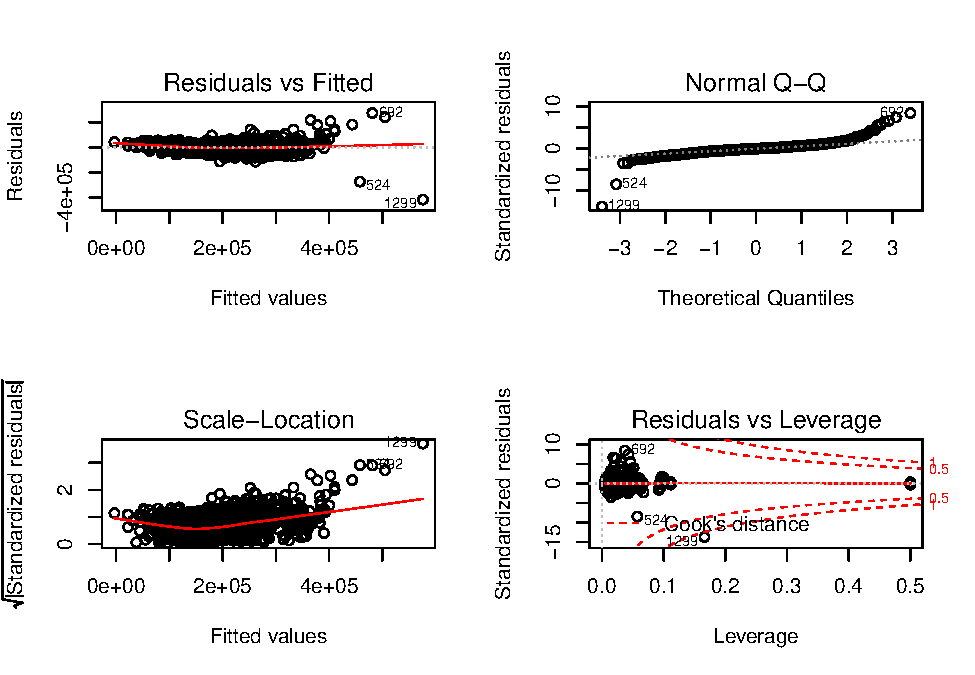
\includegraphics{Final_Project_files/figure-latex/unnamed-chunk-21-1.pdf}

\begin{Shaded}
\begin{Highlighting}[]
\KeywordTok{par}\NormalTok{(p)}
\end{Highlighting}
\end{Shaded}

I am slightly concerned that the residual plot does not look like a
shotgun pattern. My assumption is that the high influence points and/or
outliers may be impacting the model. Outlier treatment may improve the
model but the model is currently sufficient for our purposes.

\begin{Shaded}
\begin{Highlighting}[]
\KeywordTok{library}\NormalTok{(car)}
\KeywordTok{library}\NormalTok{(data.table)}
\NormalTok{lmfit <-}\StringTok{ }\KeywordTok{setDT}\NormalTok{(}\KeywordTok{as.data.frame}\NormalTok{(car::}\KeywordTok{vif}\NormalTok{(fit)), }\DataTypeTok{keep.rownames =} \OtherTok{TRUE}\NormalTok{)[]}
\NormalTok{lmfit$Adjusted_GVIF <-}\StringTok{ }\NormalTok{(lmfit$}\StringTok{`}\DataTypeTok{GVIF^(1/(2*Df))}\StringTok{`}\NormalTok{^}\DecValTok{2}\NormalTok{)}
\KeywordTok{kable}\NormalTok{(lmfit, }\DataTypeTok{align =} \KeywordTok{c}\NormalTok{(}\StringTok{"l"}\NormalTok{, }\StringTok{"c"}\NormalTok{, }\StringTok{"c"}\NormalTok{, }\StringTok{"c"}\NormalTok{, }\StringTok{"c"}\NormalTok{))}
\end{Highlighting}
\end{Shaded}

\begin{longtable}[]{@{}lcccc@{}}
\toprule
rn & GVIF & Df & GVIF\^{}(1/(2*Df)) & Adjusted\_GVIF\tabularnewline
\midrule
\endhead
MSSubClass & 1.412246 & 1 & 1.188379 & 1.412246\tabularnewline
Neighborhood & 5.575916 & 24 & 1.036450 & 1.074228\tabularnewline
OverallQual & 3.035516 & 1 & 1.742273 & 3.035516\tabularnewline
YearRemodAdd & 1.786865 & 1 & 1.336737 & 1.786865\tabularnewline
BsmtFinSF1 & 1.231322 & 1 & 1.109649 & 1.231322\tabularnewline
GrLivArea & 1.980075 & 1 & 1.407151 & 1.980075\tabularnewline
GarageCars & 1.928807 & 1 & 1.388815 & 1.928807\tabularnewline
\bottomrule
\end{longtable}

Using GVIF\^{}(1/(2*Df)) \footnote{``Which Variance Inflation Factor
  Should I Be Using: \(GVIF\) or \(text{GVIF}^{1/(2cdottext{df})}\)?''
  R. N.p., n.d. Web. 13 Nov. 2016.} in order to verify that the VIF
threshold of 5 for multicollinearity is not exceed. Fortunately, we find
that no variable exceeds the threshold and we do not need to adjust for
multicollinearity.

\subsection{The final model}\label{the-final-model}

Provide your complete model summary and results with analysis.

\begin{Shaded}
\begin{Highlighting}[]
\KeywordTok{stargazer}\NormalTok{(fit, }\DataTypeTok{header =} \OtherTok{FALSE}\NormalTok{, }\DataTypeTok{no.space =} \OtherTok{TRUE}\NormalTok{, }
          \DataTypeTok{style =} \StringTok{"all2"}\NormalTok{, }\DataTypeTok{font.size =} \StringTok{"normalsize"}\NormalTok{, }
          \DataTypeTok{single.row =} \OtherTok{TRUE}\NormalTok{, }\DataTypeTok{intercept.bottom =} \OtherTok{FALSE}\NormalTok{)}
\end{Highlighting}
\end{Shaded}

\begin{table}[!htbp] \centering 
  \caption{} 
  \label{} 
\normalsize 
\begin{tabular}{@{\extracolsep{5pt}}lc} 
\\[-1.8ex]\hline 
\hline \\[-1.8ex] 
 & \multicolumn{1}{c}{\textit{Dependent variable:}} \\ 
\cline{2-2} 
\\[-1.8ex] & SalePrice \\ 
\hline \\[-1.8ex] 
 Constant & $-$621,777.700$^{***}$ (111,442.300) \\ 
  MSSubClass & $-$252.678$^{***}$ (24.405) \\ 
  NeighborhoodBlueste & $-$12,510.880 (24,882.880) \\ 
  NeighborhoodBrDale & $-$16,417.030 (11,866.240) \\ 
  NeighborhoodBrkSide & $-$14,640.440 (9,753.068) \\ 
  NeighborhoodClearCr & 7,771.633 (10,647.930) \\ 
  NeighborhoodCollgCr & $-$8,855.995 (8,742.258) \\ 
  NeighborhoodCrawfor & 7,447.104 (9,729.488) \\ 
  NeighborhoodEdwards & $-$24,629.000$^{***}$ (9,317.138) \\ 
  NeighborhoodGilbert & $-$12,303.590 (9,065.933) \\ 
  NeighborhoodIDOTRR & $-$25,820.490$^{**}$ (10,379.870) \\ 
  NeighborhoodMeadowV & 1,205.989 (11,879.710) \\ 
  NeighborhoodMitchel & $-$18,072.460$^{*}$ (9,692.696) \\ 
  NeighborhoodNAmes & $-$18,834.730$^{**}$ (8,971.063) \\ 
  NeighborhoodNoRidge & 40,530.480$^{***}$ (10,050.780) \\ 
  NeighborhoodNPkVill & $-$9,409.847 (13,823.590) \\ 
  NeighborhoodNridgHt & 49,514.520$^{***}$ (9,100.426) \\ 
  NeighborhoodNWAmes & $-$21,429.510$^{**}$ (9,344.861) \\ 
  NeighborhoodOldTown & $-$31,650.010$^{***}$ (9,111.020) \\ 
  NeighborhoodSawyer & $-$19,047.140$^{**}$ (9,502.205) \\ 
  NeighborhoodSawyerW & $-$15,759.290$^{*}$ (9,404.611) \\ 
  NeighborhoodSomerst & 7,011.384 (8,880.182) \\ 
  NeighborhoodStoneBr & 55,104.420$^{***}$ (10,602.380) \\ 
  NeighborhoodSWISU & $-$27,693.620$^{**}$ (11,081.320) \\ 
  NeighborhoodTimber & 3,500.186 (9,974.428) \\ 
  NeighborhoodVeenker & 25,505.000$^{*}$ (13,027.270) \\ 
  OverallQual & 16,039.450$^{***}$ (1,094.370) \\ 
  YearRemodAdd & 310.102$^{***}$ (56.246) \\ 
  BsmtFinSF1 & 23.326$^{***}$ (2.113) \\ 
  GrLivArea & 52.970$^{***}$ (2.326) \\ 
  GarageCars & 11,974.750$^{***}$ (1,614.394) \\ 
 \hline \\[-1.8ex] 
Observations & 1,460 \\ 
R$^{2}$ & 0.829 \\ 
Adjusted R$^{2}$ & 0.826 \\ 
Residual Std. Error & 33,181.540 (df = 1429) \\ 
F Statistic & 231.137$^{***}$ (df = 30; 1429)  (p = 0.000) \\ 
\hline 
\hline \\[-1.8ex] 
\textit{Note:}  & \multicolumn{1}{r}{$^{*}$p$<$0.1; $^{**}$p$<$0.05; $^{***}$p$<$0.01} \\ 
\end{tabular} 
\end{table}

Prediction results with test data set

\begin{Shaded}
\begin{Highlighting}[]
\NormalTok{test.df  <-}\StringTok{ }\KeywordTok{as_tibble}\NormalTok{(}\KeywordTok{read.csv}\NormalTok{(}\KeywordTok{paste}\NormalTok{(}\StringTok{"https://raw.githubusercontent.com/"}\NormalTok{, }\StringTok{"ChristopheHunt/"}\NormalTok{,}
                                      \StringTok{"MSDA---Coursework/master"}\NormalTok{, }
                                      \StringTok{"/Data%20605/Final%20Project/test.csv"}\NormalTok{, }\DataTypeTok{sep =} \StringTok{""}\NormalTok{)))}

\NormalTok{SalePrice.predict <-}\StringTok{ }\KeywordTok{predict.lm}\NormalTok{(fit, }\DataTypeTok{type =} \StringTok{"response"}\NormalTok{, }\DataTypeTok{newdata =} \NormalTok{test.df)}
\NormalTok{test.df.wpredict <-}\StringTok{ }\KeywordTok{cbind}\NormalTok{(test.df %>%}\StringTok{ }\NormalTok{dplyr::}\KeywordTok{select}\NormalTok{(Id), }\KeywordTok{round}\NormalTok{(SalePrice.predict,}\DecValTok{0}\NormalTok{)) }
\KeywordTok{colnames}\NormalTok{(test.df.wpredict)[}\DecValTok{2}\NormalTok{] <-}\StringTok{ }\KeywordTok{c}\NormalTok{(}\StringTok{"SalePrice"}\NormalTok{)}
\KeywordTok{pandoc.table}\NormalTok{(}\KeywordTok{head}\NormalTok{(test.df.wpredict), }\DataTypeTok{split.table =} \OtherTok{Inf}\NormalTok{)}
\end{Highlighting}
\end{Shaded}

\begin{verbatim}
## 
## ----------------
##  Id   SalePrice 
## ---- -----------
## 1461   112993   
## 
## 1462   161652   
## 
## 1463   179227   
## 
## 1464   189533   
## 
## 1465   246930   
## 
## 1466   176952   
## ----------------
\end{verbatim}

\begin{Shaded}
\begin{Highlighting}[]
\NormalTok{gz1 <-}\StringTok{ }\KeywordTok{gzfile}\NormalTok{(}\StringTok{"submission.csv.gz"}\NormalTok{, }\StringTok{"w"}\NormalTok{)}
\KeywordTok{write.csv}\NormalTok{(test.df.wpredict, gz1, }\DataTypeTok{row.names =} \OtherTok{FALSE}\NormalTok{)}
\KeywordTok{close}\NormalTok{(gz1)}
\end{Highlighting}
\end{Shaded}

Kaggle.com user name : Kaggle.com score :


\end{document}
